\section{APPENDIX: Fit Plots of electron-photon invariant mass}
\label{sec:EtogammaFitPlots}

Fit results of $e \rightarrow \gamma$ data-driven estimation.

% On all the plots, black is data, green is $T_{true}$, blue is $T_{fake}$, and red is $F_{fit}$. The $\Chi^2/{NDF}$ quoted on the plots is computed as the $\Chi^2$ value provided by RooFit tools (RooChi2Var chi2("chi2","chi2",fullPdf,dataHist)) divided over $N_{bins}-2$ where $N_{bins}$ is the number of bins in the histogram used for fit.
  

%\begin{figure}[htb]
%  \begin{center}
%   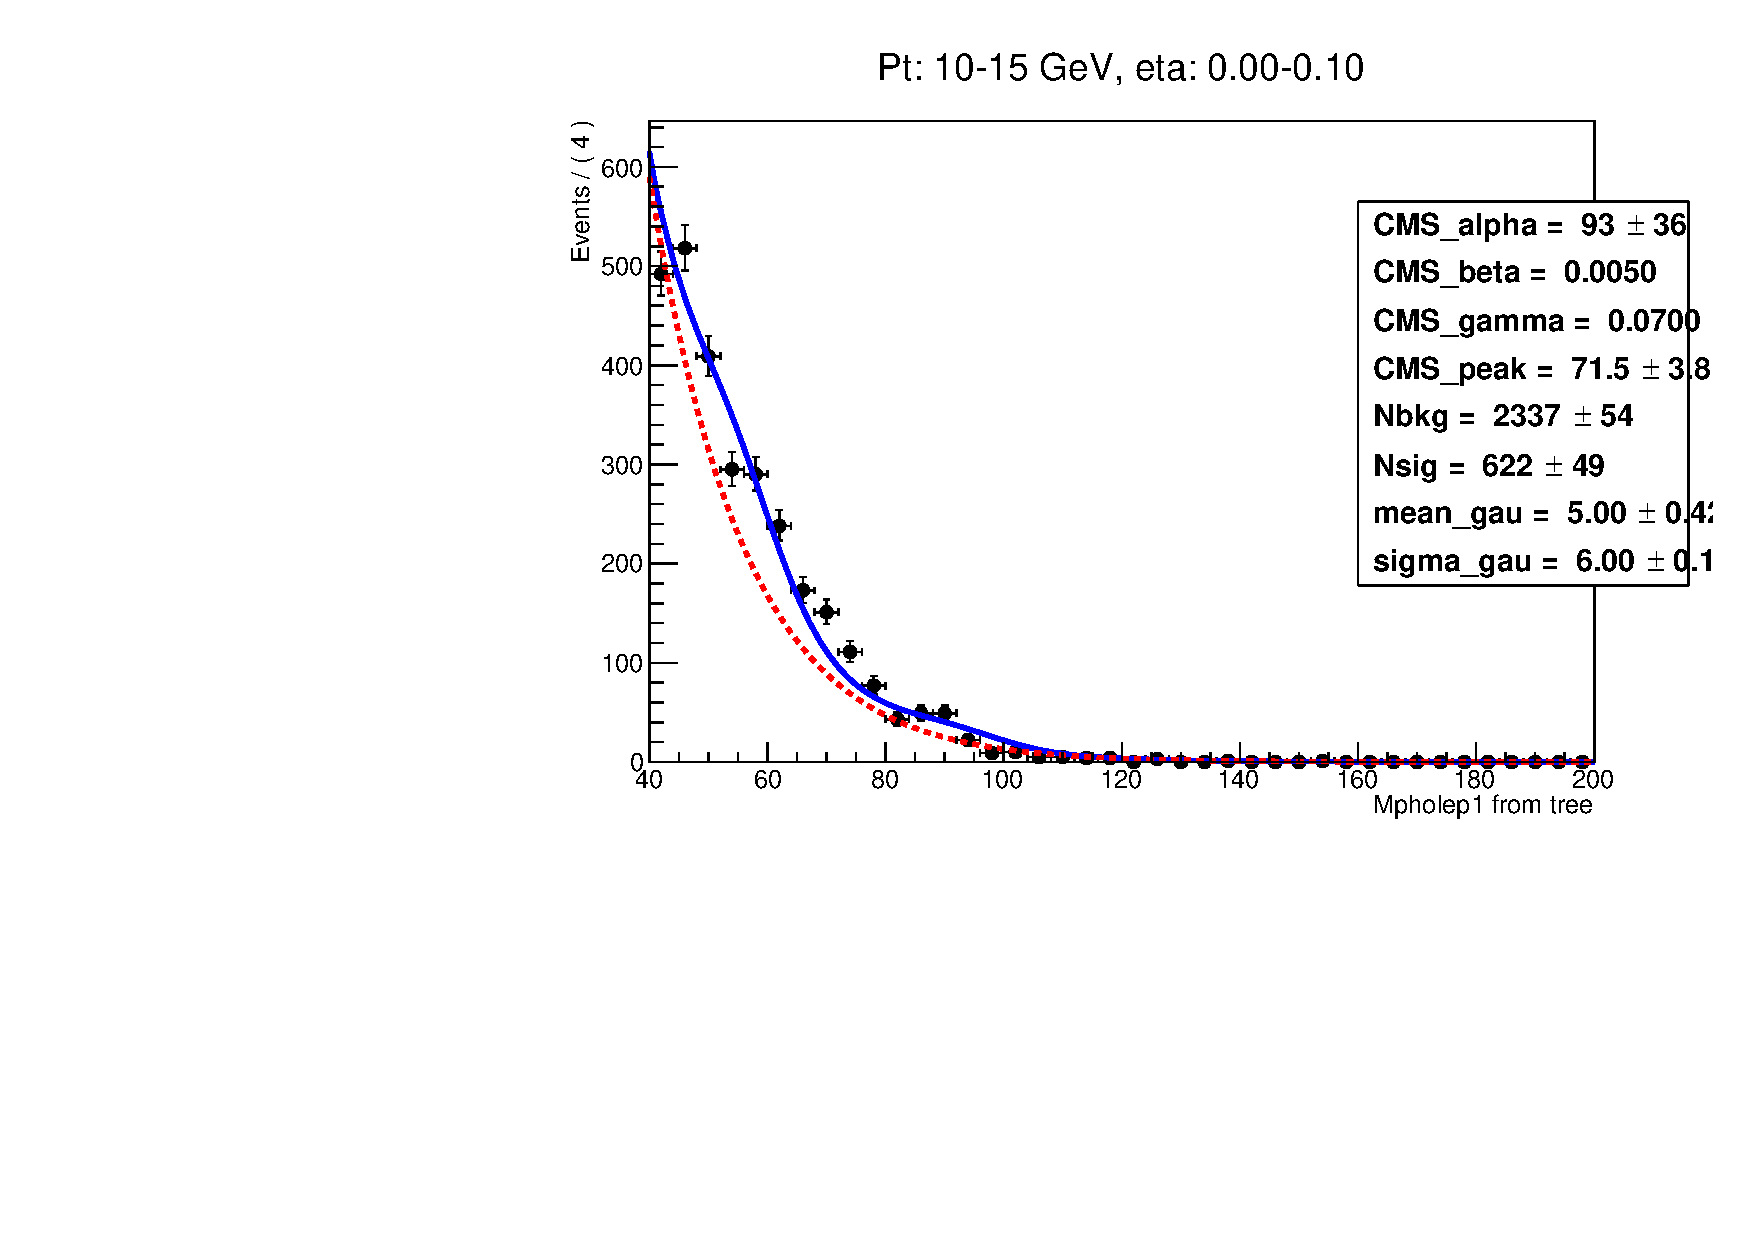
\includegraphics[width=0.45\textwidth]{../figs/figs_v11/ELECTRON_WGamma/EtoGammaFits/sa_hZmass_h_Data_EtoGamma_Enr_BARREL_pt10to15_ieta0.pdf}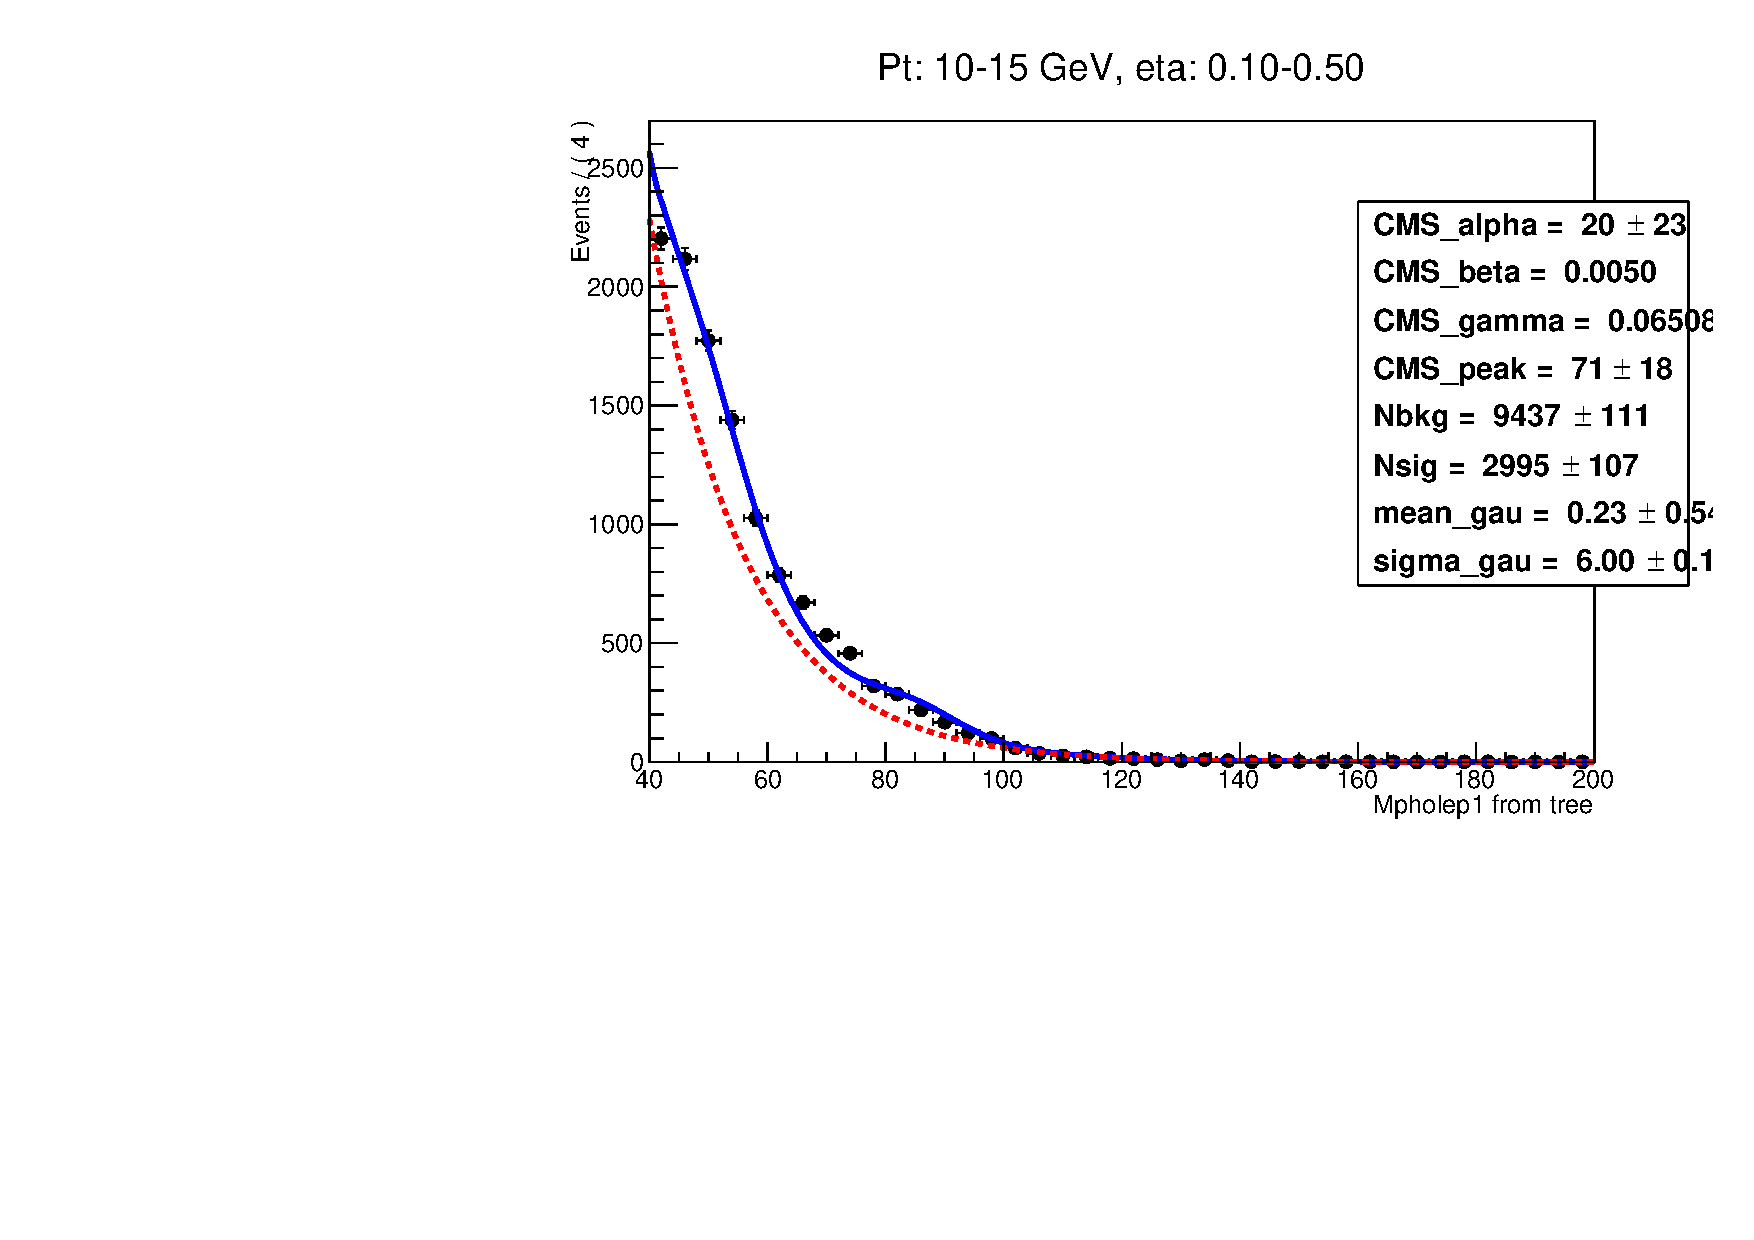
\includegraphics[width=0.45\textwidth]{../figs/figs_v11/ELECTRON_WGamma/EtoGammaFits/sa_hZmass_h_Data_EtoGamma_Enr_BARREL_pt10to15_ieta1.pdf}\\
%   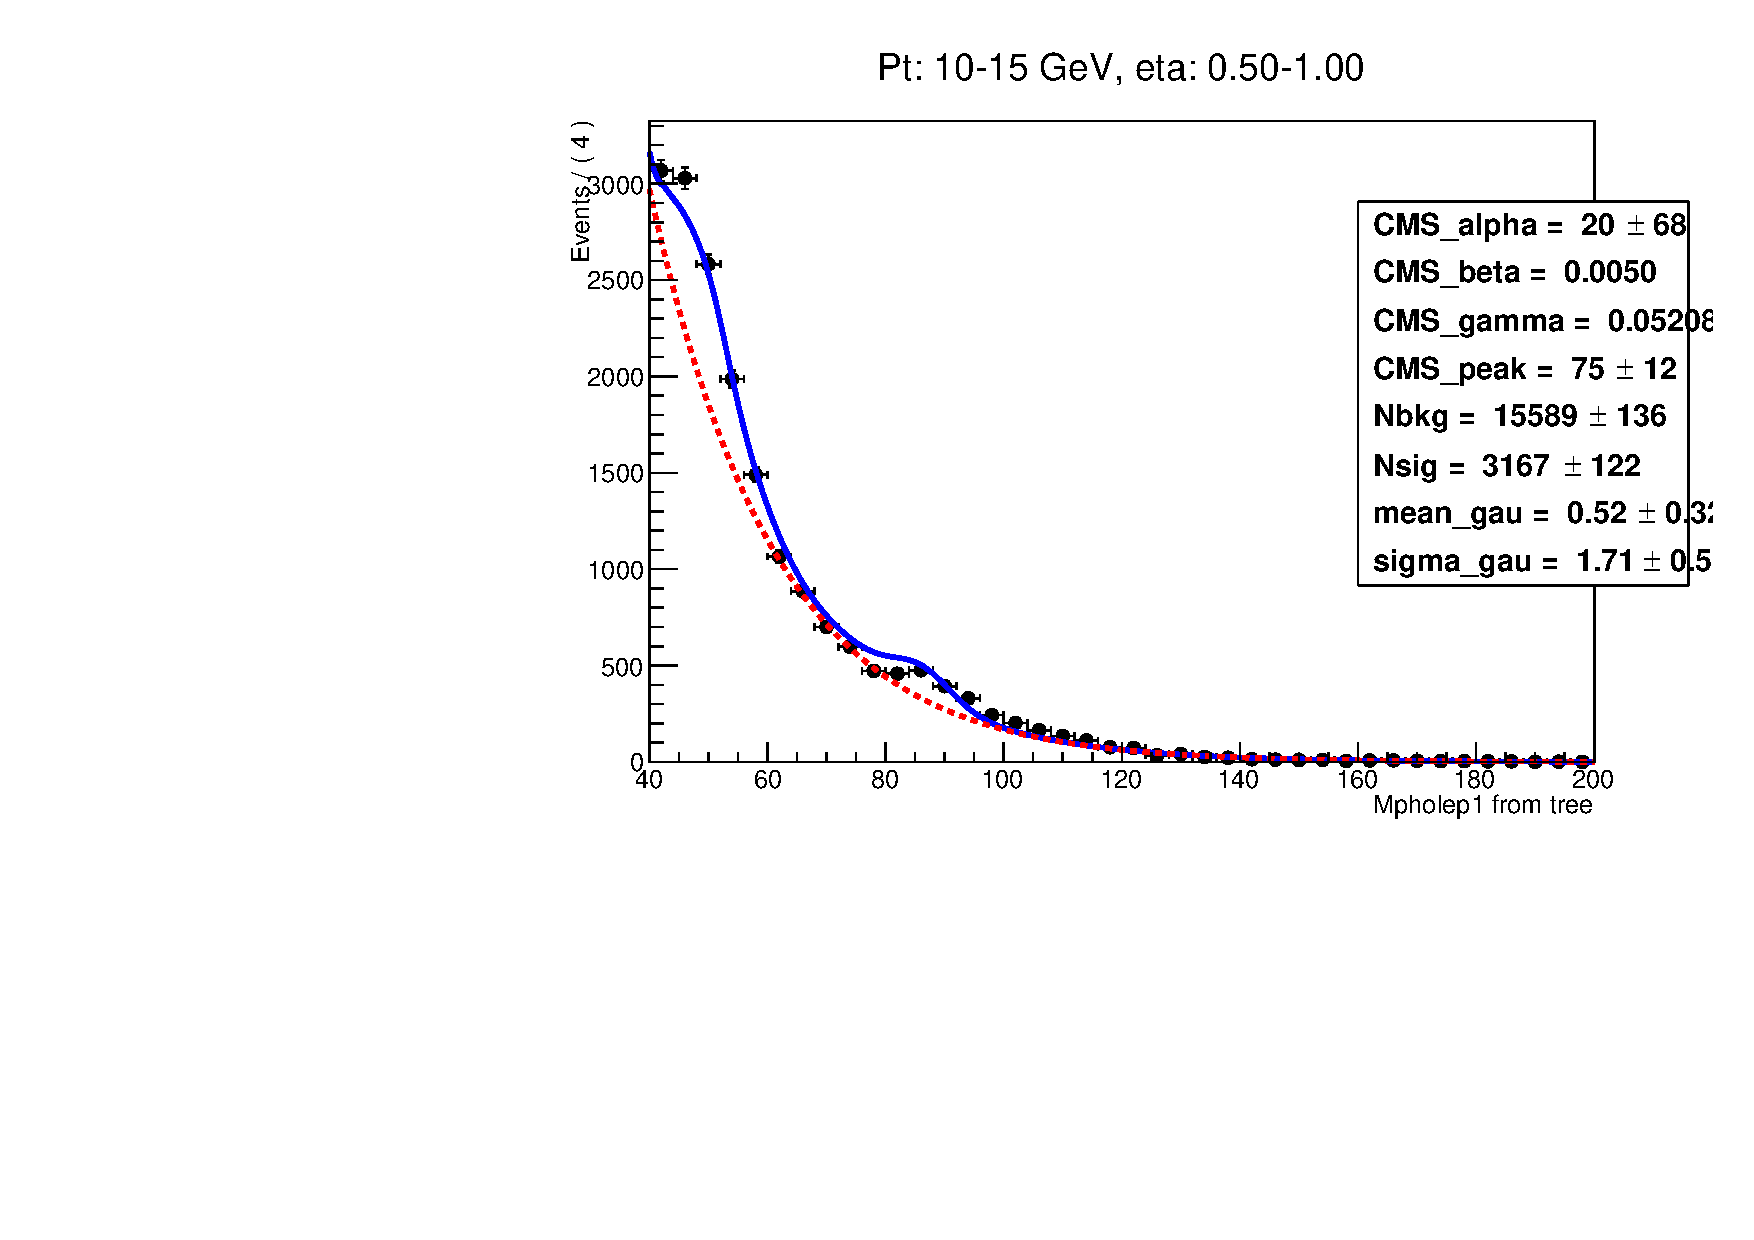
\includegraphics[width=0.45\textwidth]{../figs/figs_v11/ELECTRON_WGamma/EtoGammaFits/sa_hZmass_h_Data_EtoGamma_Enr_BARREL_pt10to15_ieta2.pdf}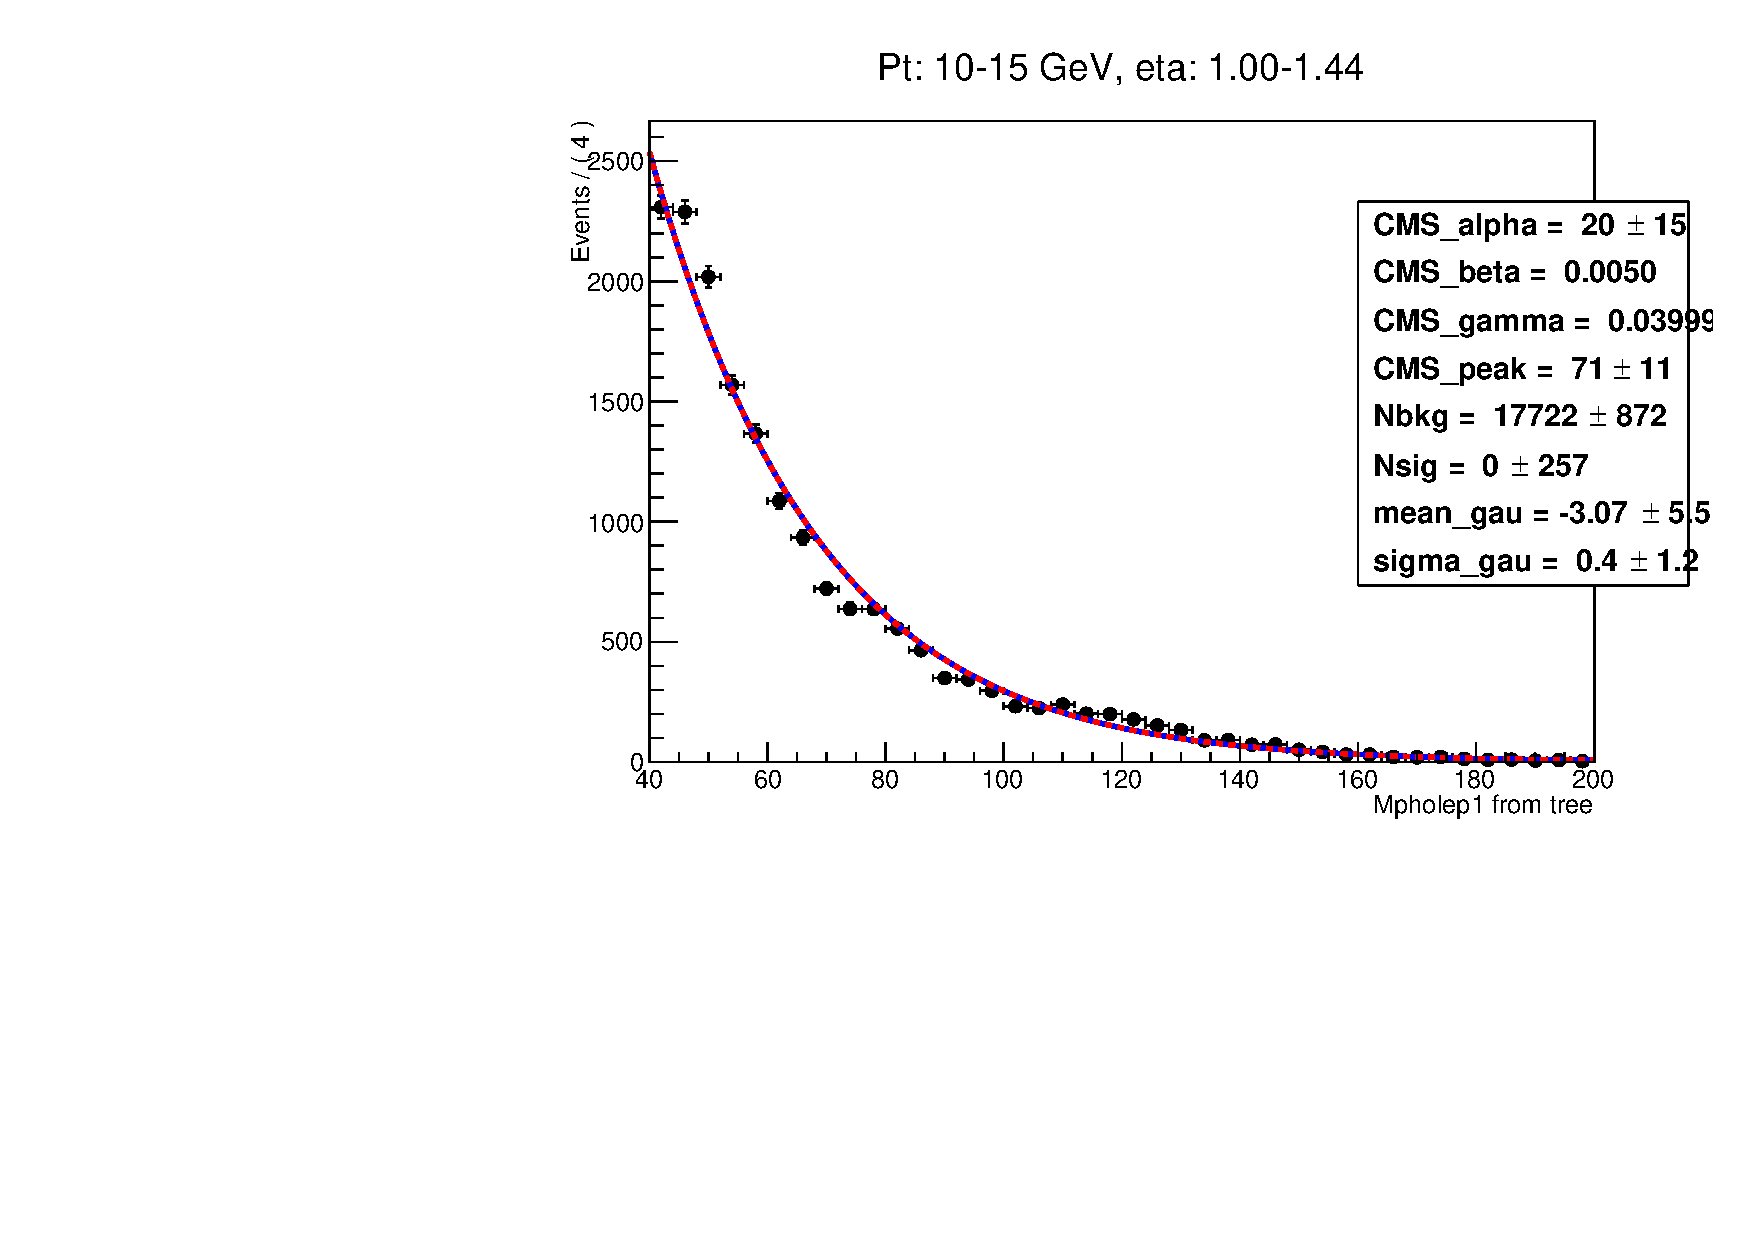
\includegraphics[width=0.45\textwidth]{../figs/figs_v11/ELECTRON_WGamma/EtoGammaFits/sa_hZmass_h_Data_EtoGamma_Enr_BARREL_pt10to15_ieta3.pdf}\\
%   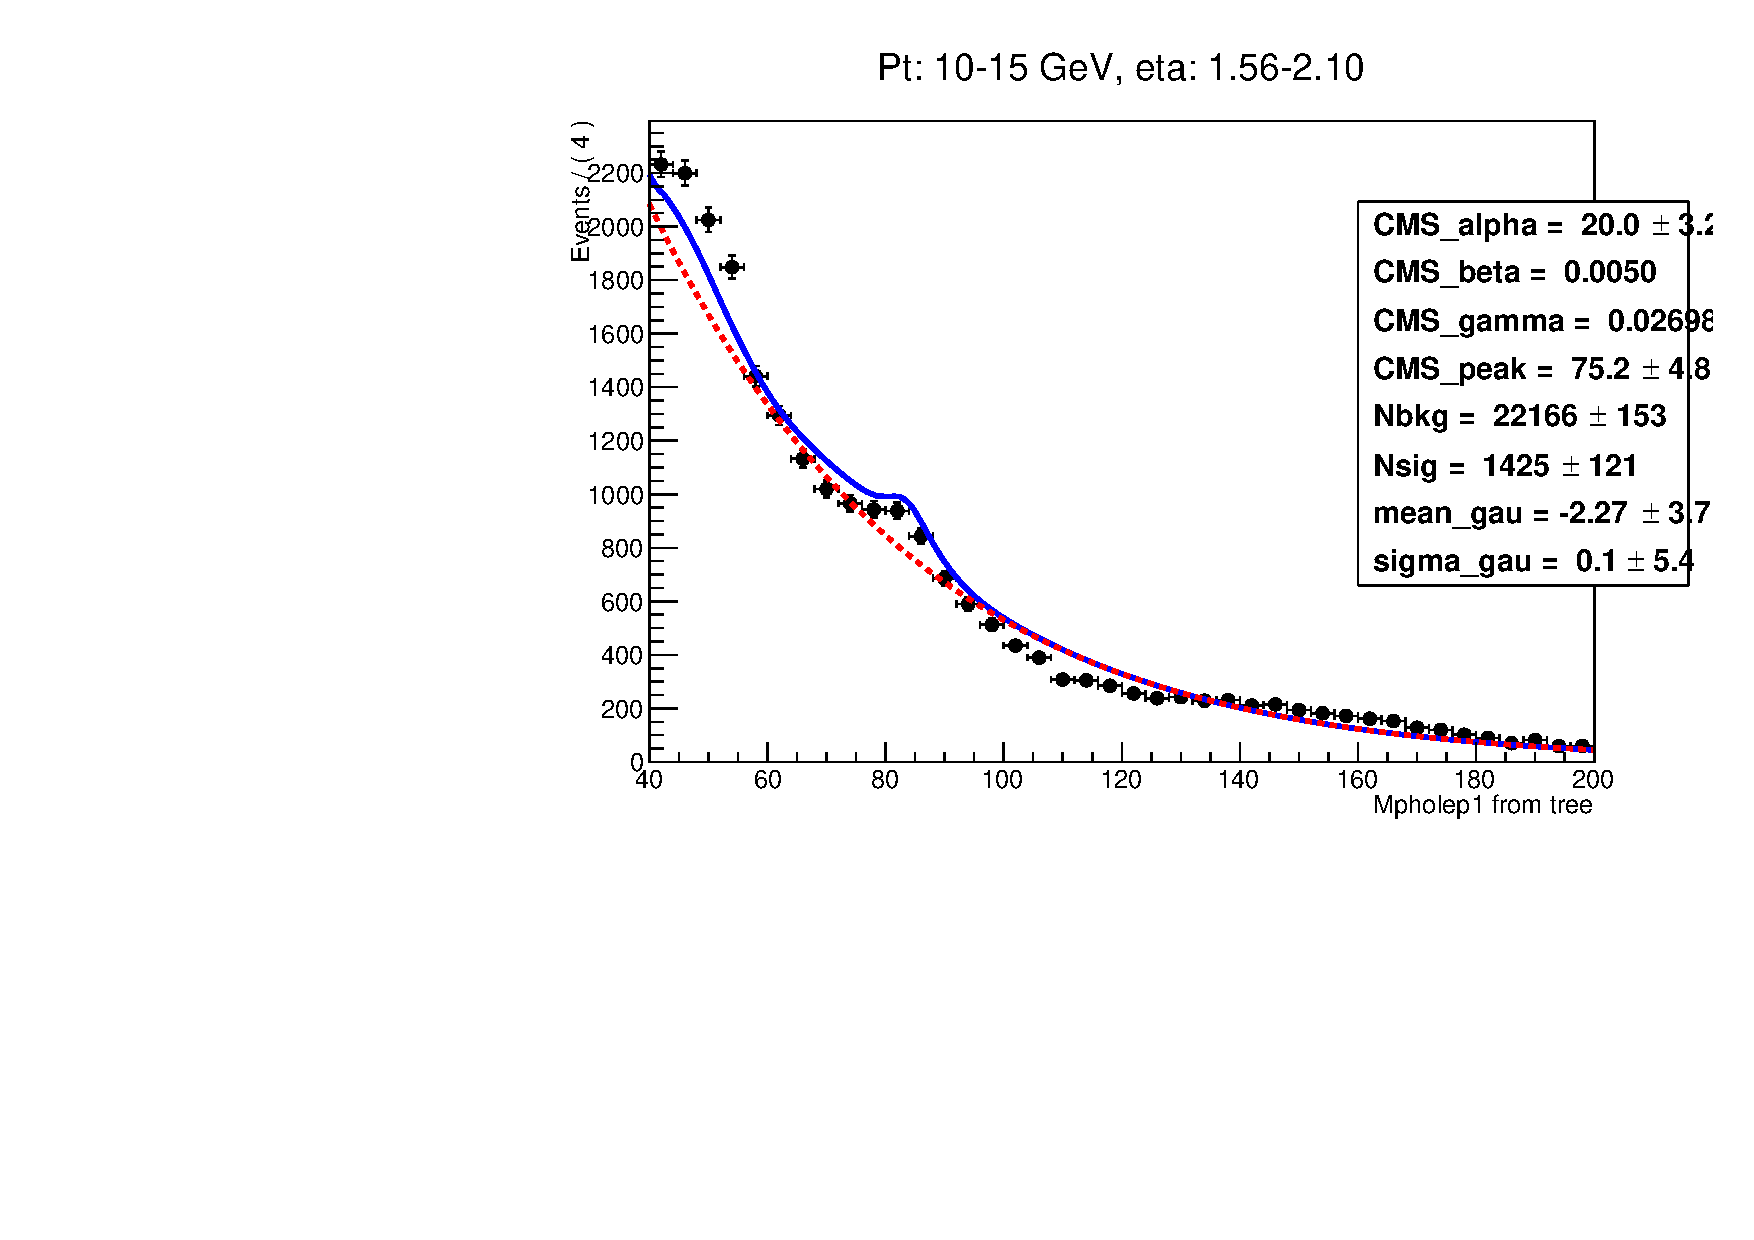
\includegraphics[width=0.45\textwidth]{../figs/figs_v11/ELECTRON_WGamma/EtoGammaFits/sa_hZmass_h_Data_EtoGamma_Enr_ENDCAP_pt10to15_ieta0.pdf}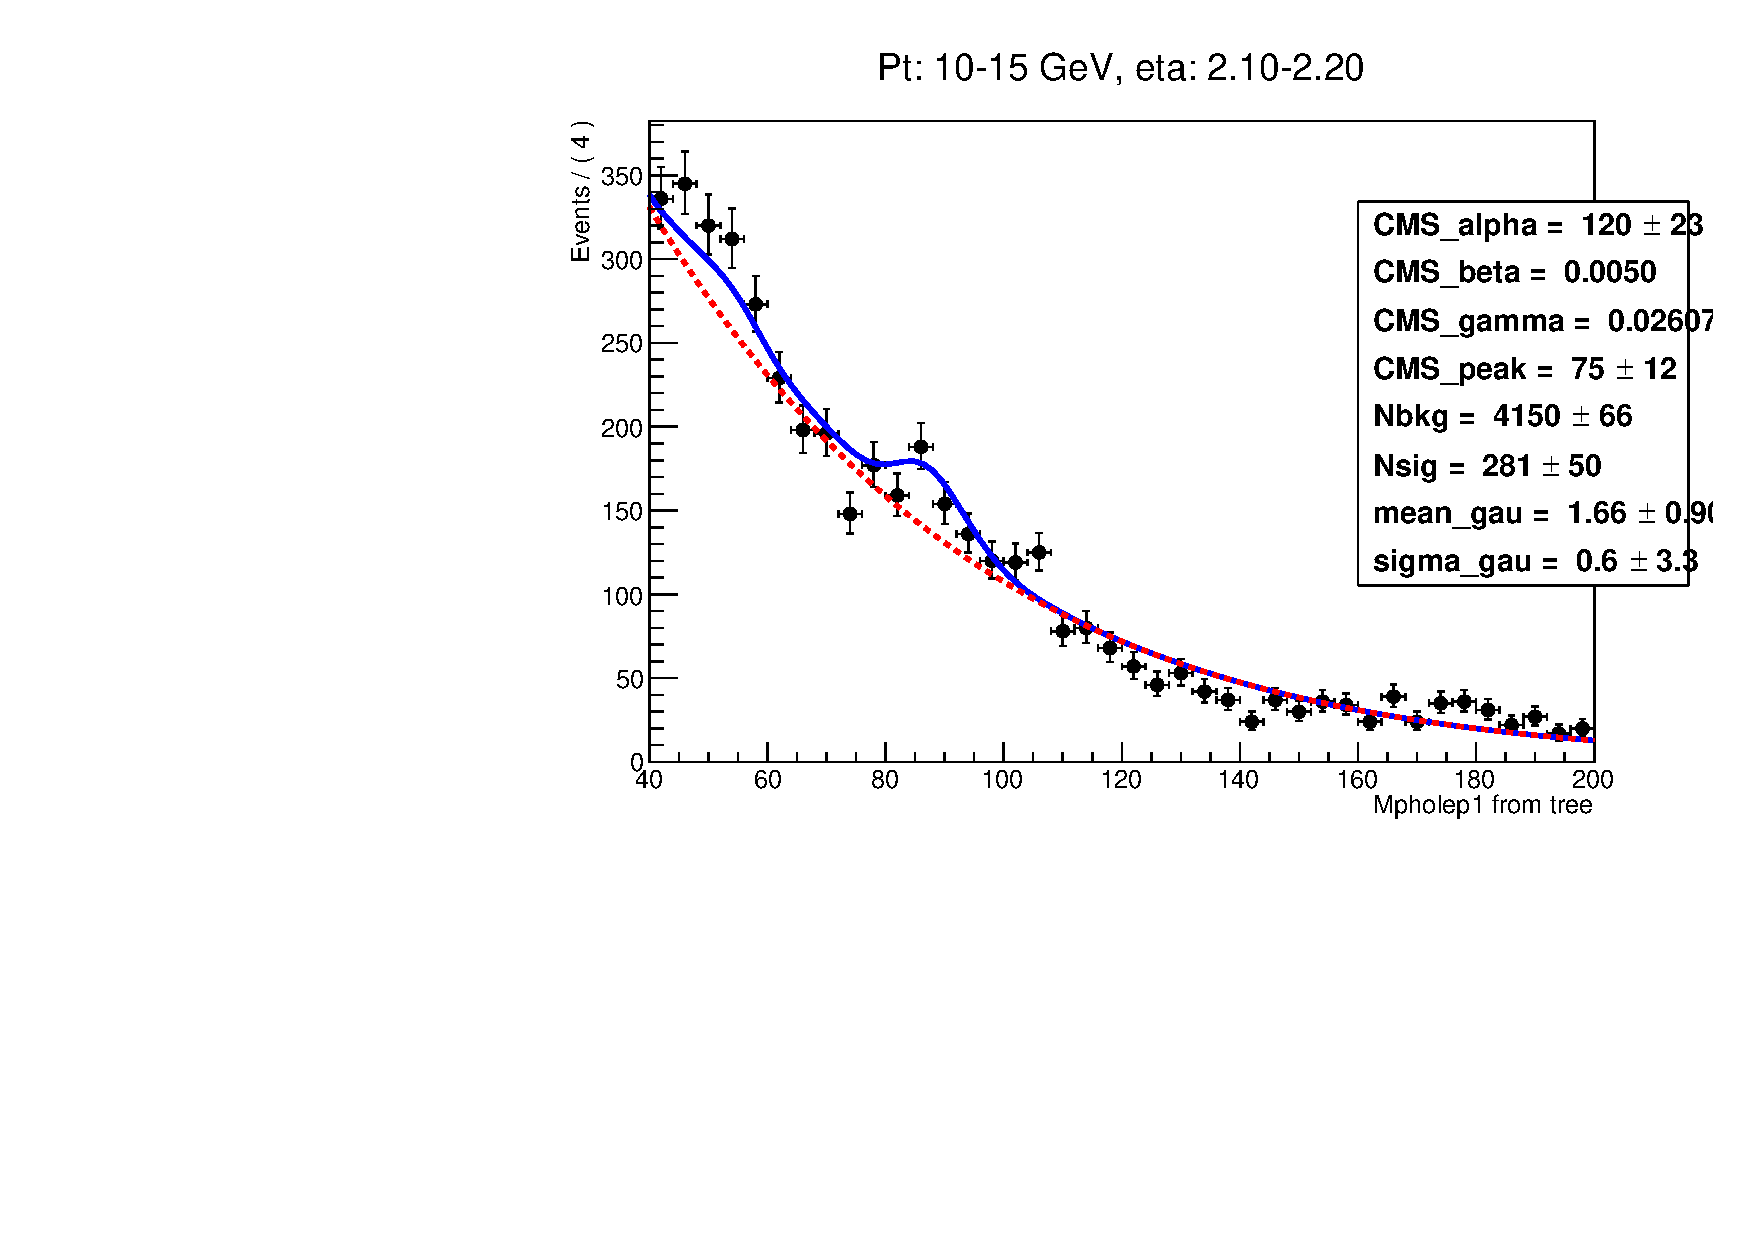
\includegraphics[width=0.45\textwidth]{../figs/figs_v11/ELECTRON_WGamma/EtoGammaFits/sa_hZmass_h_Data_EtoGamma_Enr_ENDCAP_pt10to15_ieta1.pdf}\\
%   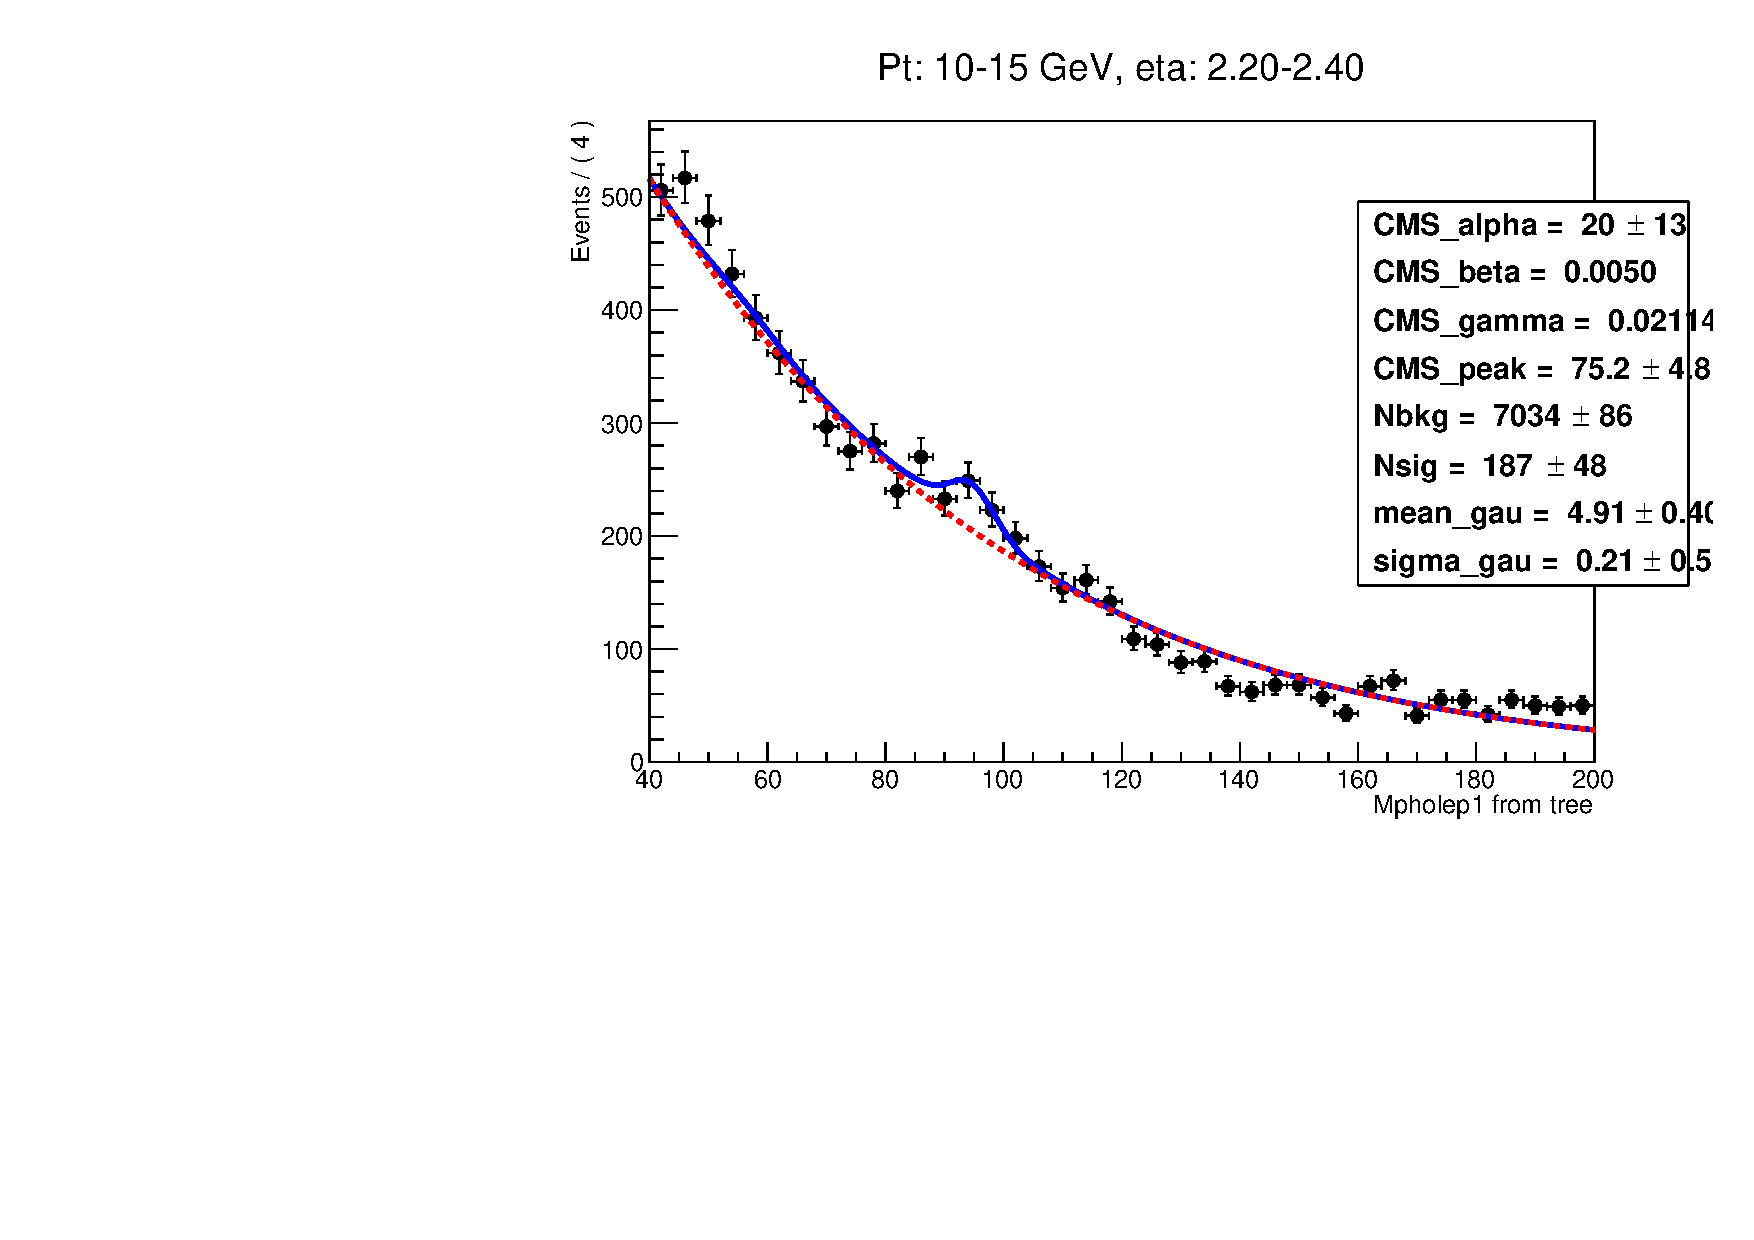
\includegraphics[width=0.45\textwidth]{../figs/figs_v11/ELECTRON_WGamma/EtoGammaFits/sa_hZmass_h_Data_EtoGamma_Enr_ENDCAP_pt10to15_ieta2.pdf}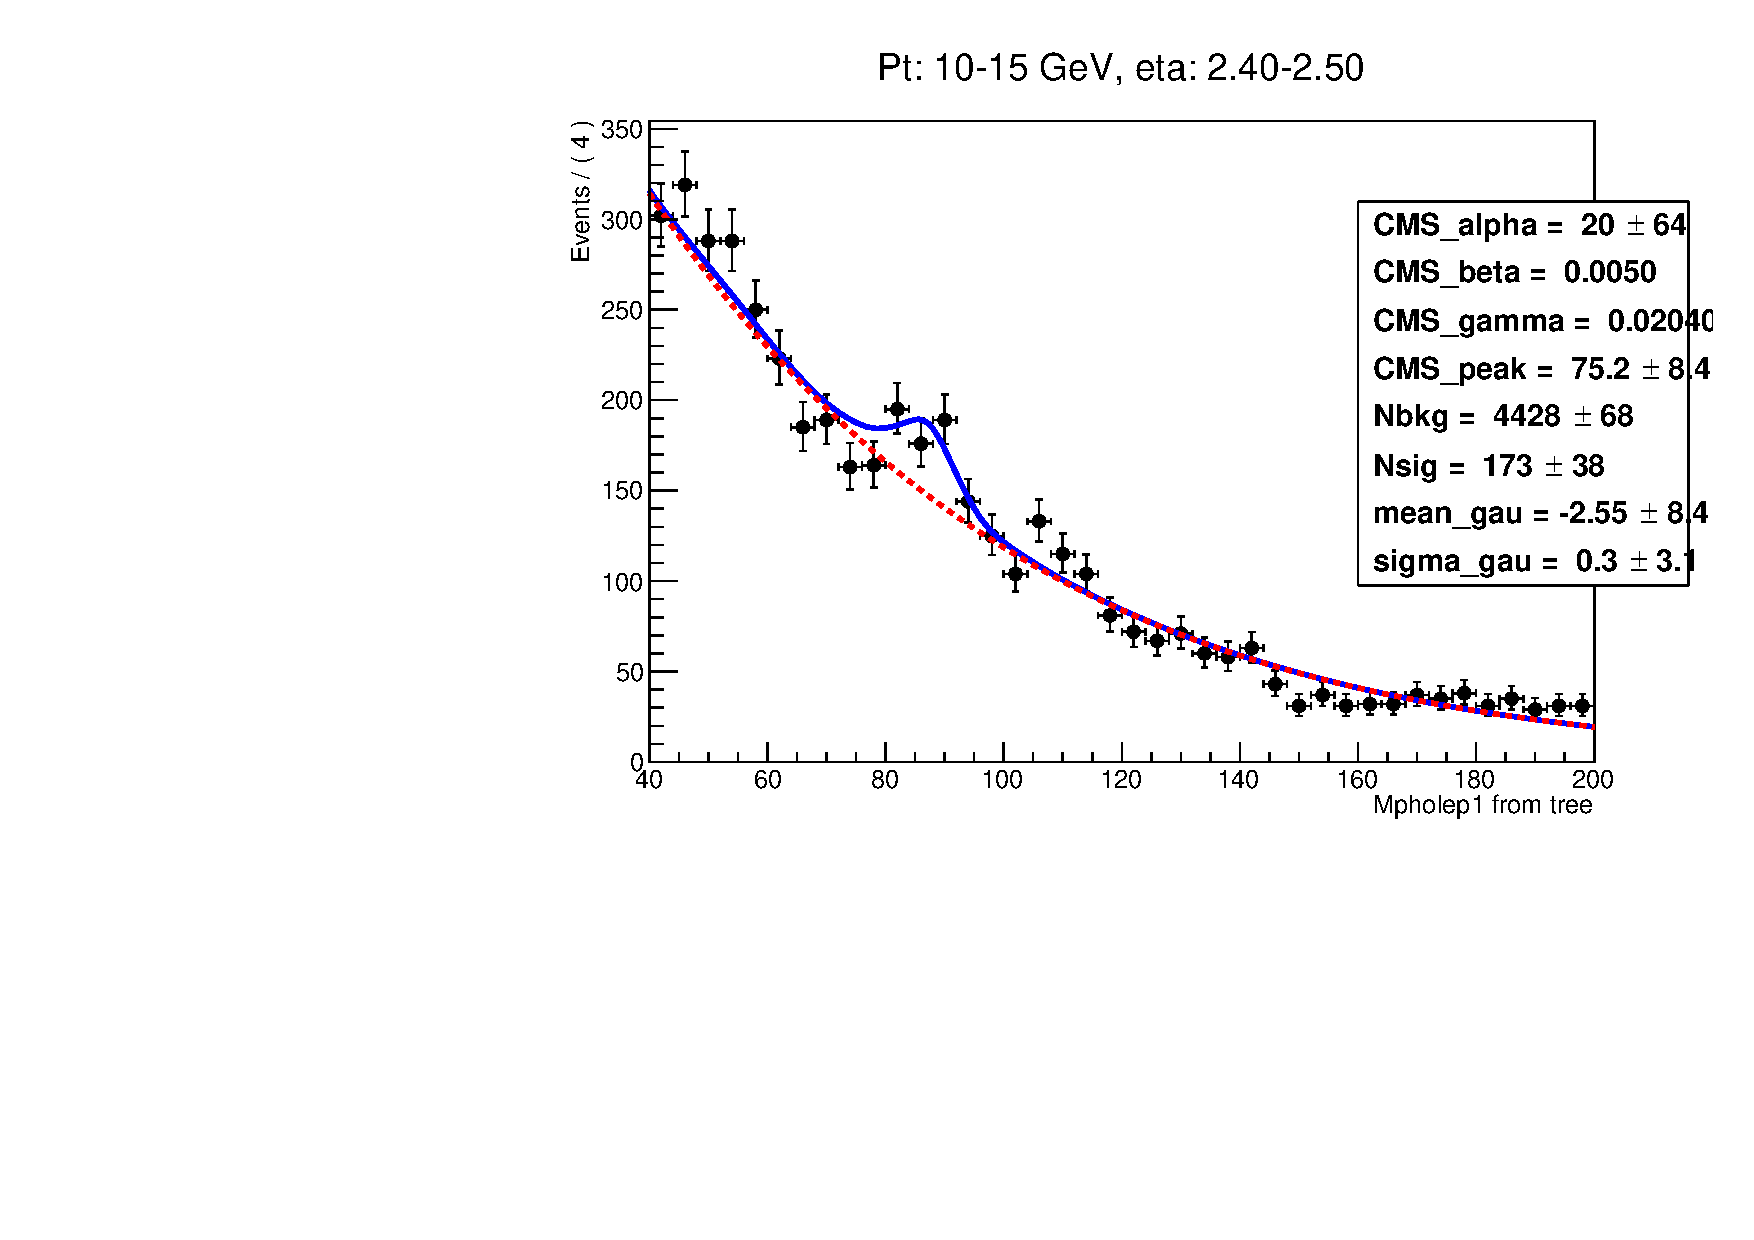
\includegraphics[width=0.45\textwidth]{../figs/figs_v11/ELECTRON_WGamma/EtoGammaFits/sa_hZmass_h_Data_EtoGamma_Enr_ENDCAP_pt10to15_ieta3.pdf}\\
%  \label{fig:etogFits_10to15}
%  \caption{$M_{e,\gamma}$ fits, W$\gamma$, electron channel, underflow bin (10-15 GeV), 8 eta bins}
%  \end{center}
%\end{figure}

\begin{figure}[htb]
  \begin{center}
   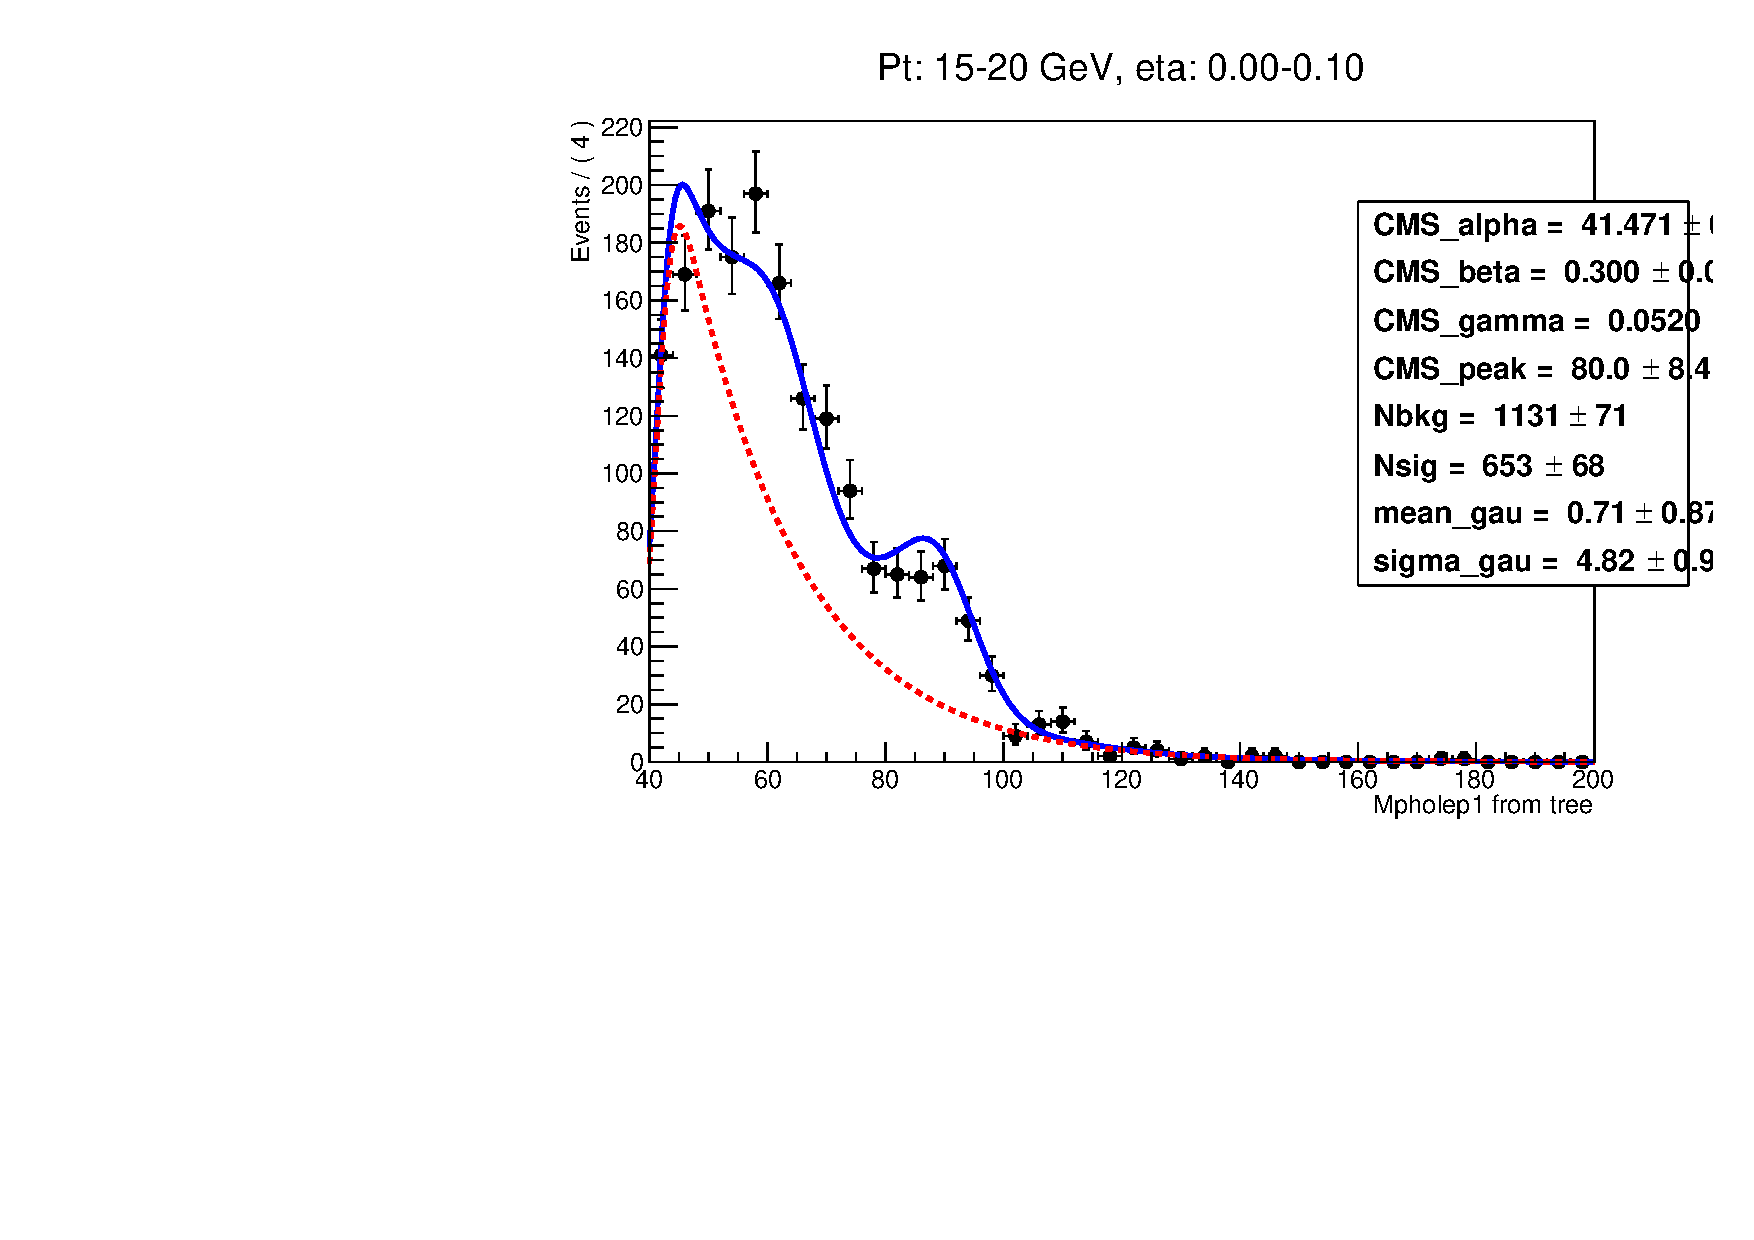
\includegraphics[width=0.45\textwidth]{../figs/figs_v11/ELECTRON_WGamma/EtoGammaFits/sa_hZmass_h_Data_EtoGamma_Enr_BARREL_pt15to20_ieta0.pdf}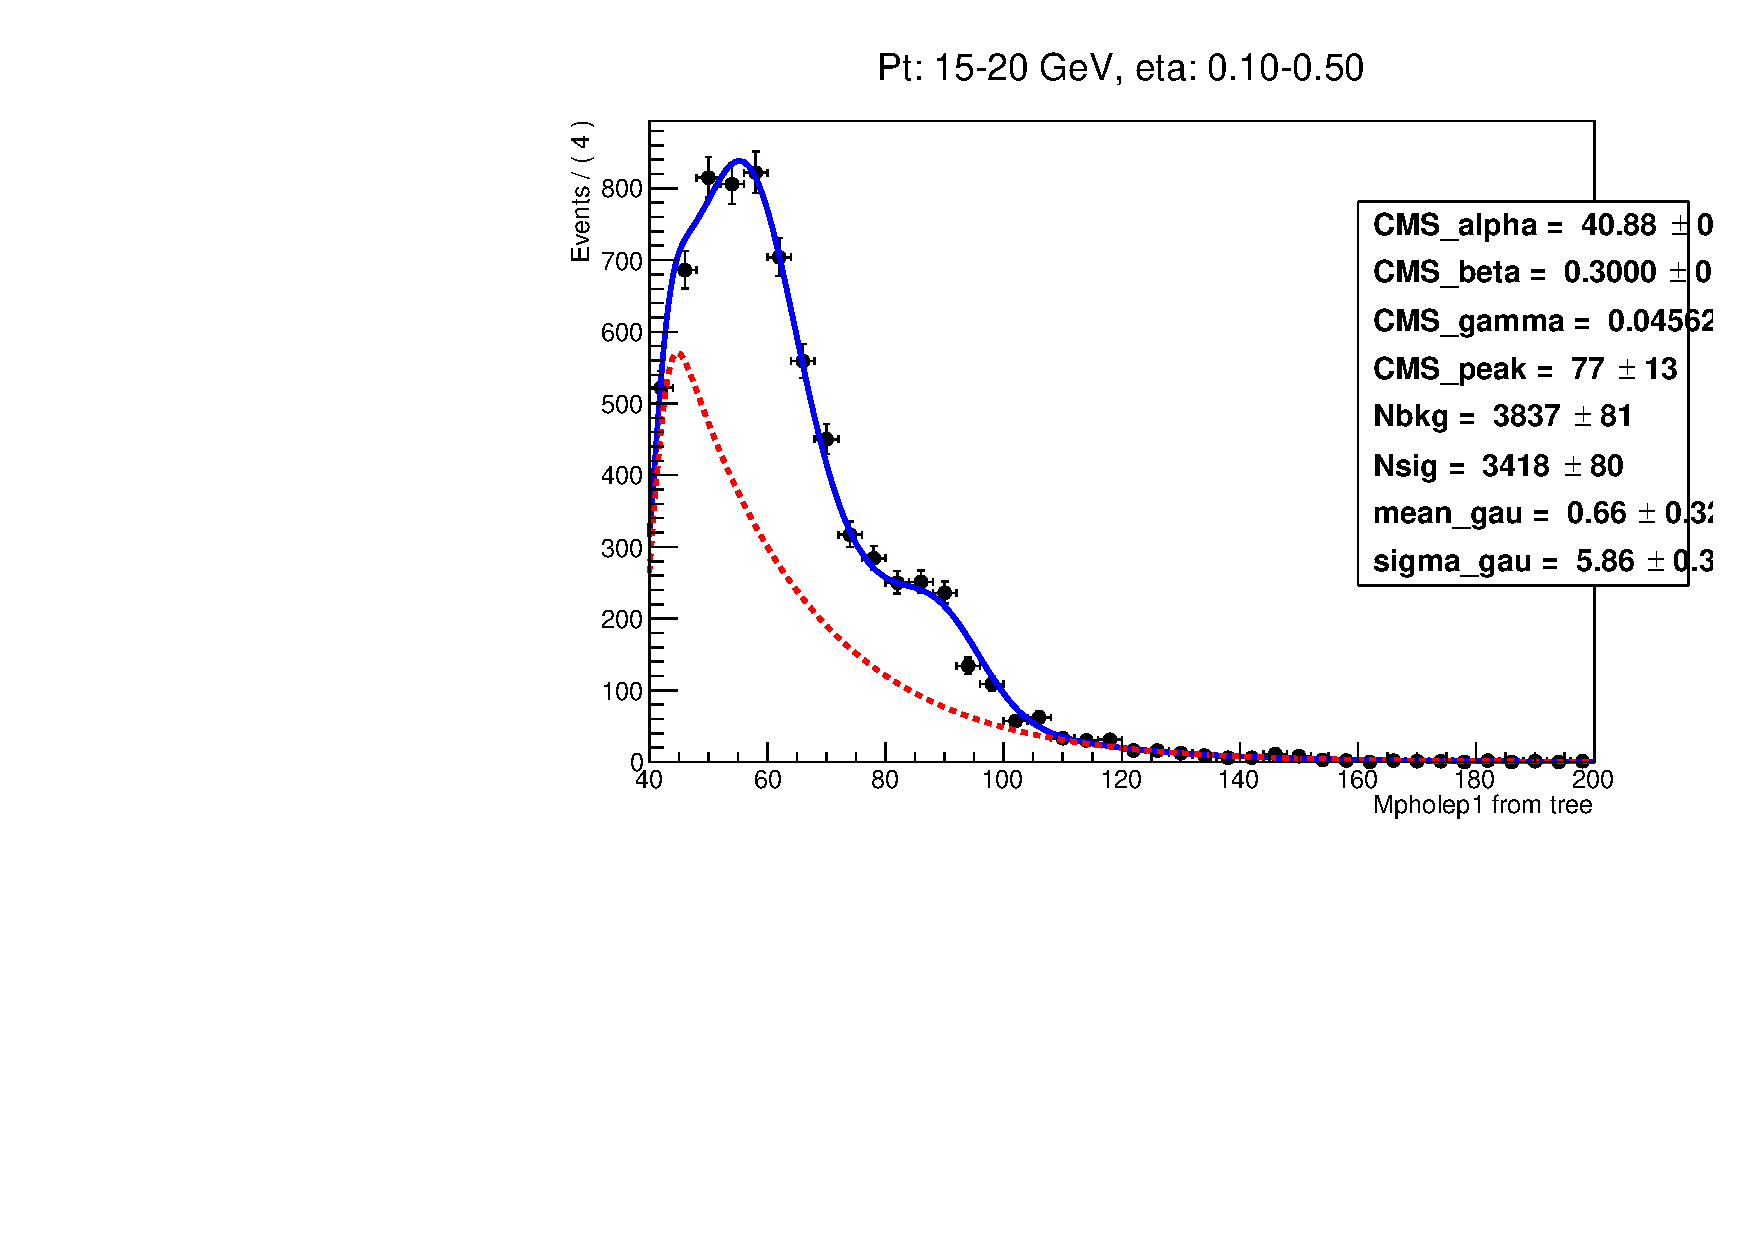
\includegraphics[width=0.45\textwidth]{../figs/figs_v11/ELECTRON_WGamma/EtoGammaFits/sa_hZmass_h_Data_EtoGamma_Enr_BARREL_pt15to20_ieta1.pdf}\\
   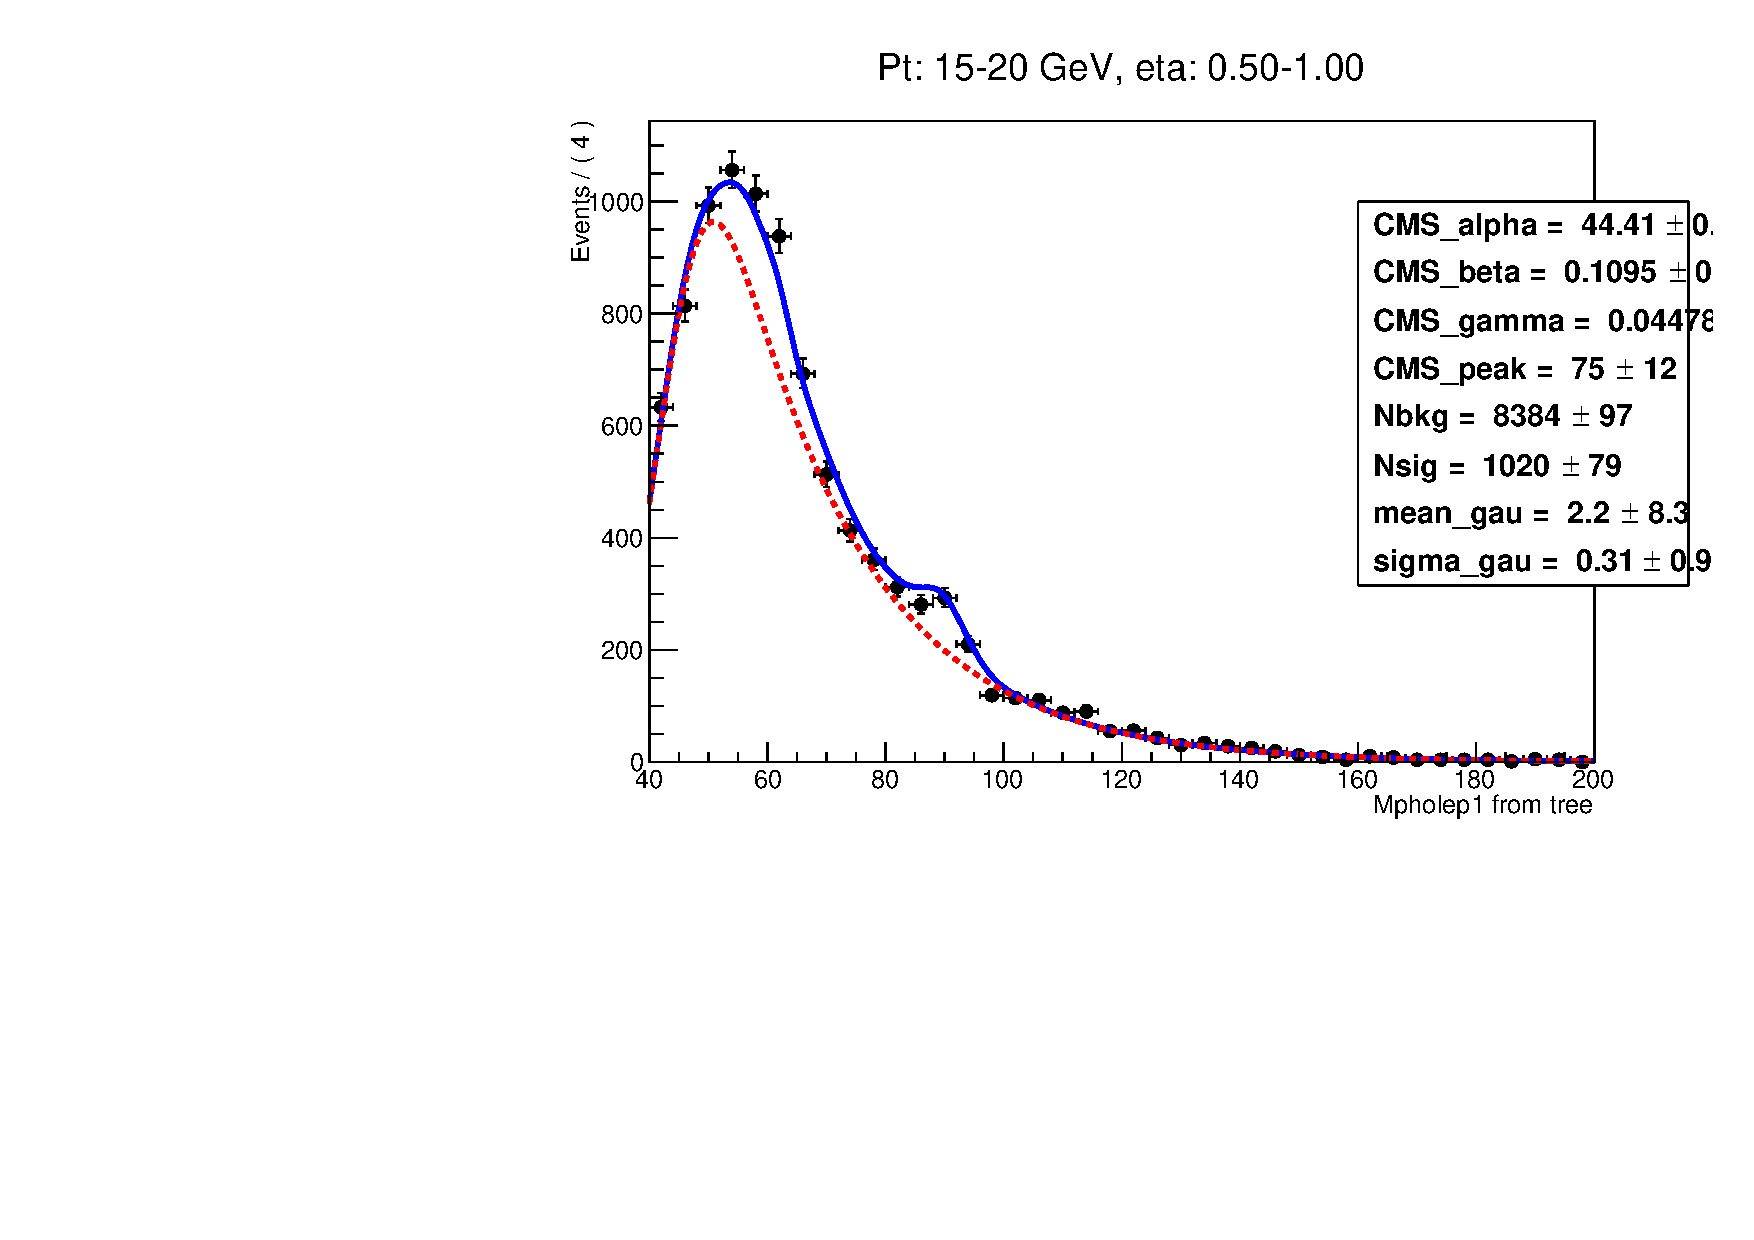
\includegraphics[width=0.45\textwidth]{../figs/figs_v11/ELECTRON_WGamma/EtoGammaFits/sa_hZmass_h_Data_EtoGamma_Enr_BARREL_pt15to20_ieta2.pdf}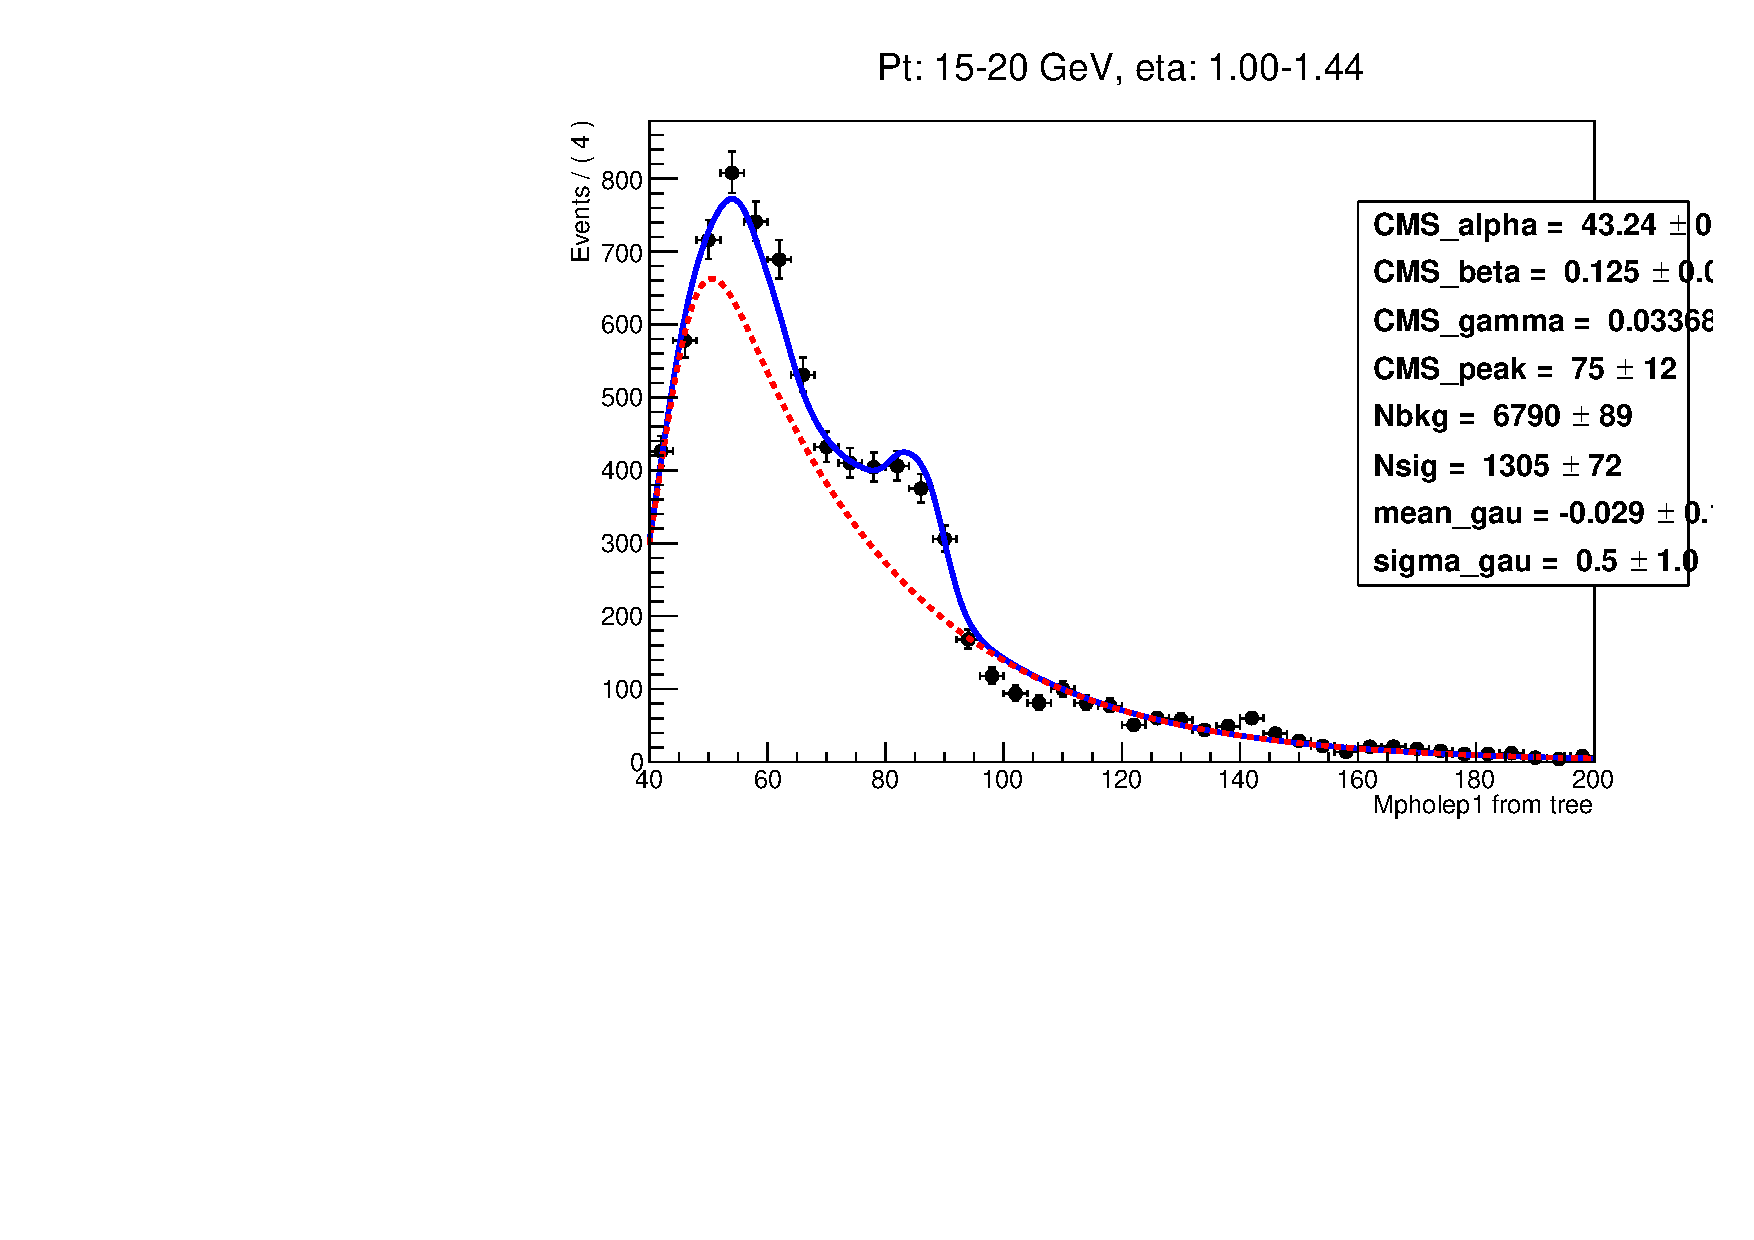
\includegraphics[width=0.45\textwidth]{../figs/figs_v11/ELECTRON_WGamma/EtoGammaFits/sa_hZmass_h_Data_EtoGamma_Enr_BARREL_pt15to20_ieta3.pdf}\\
   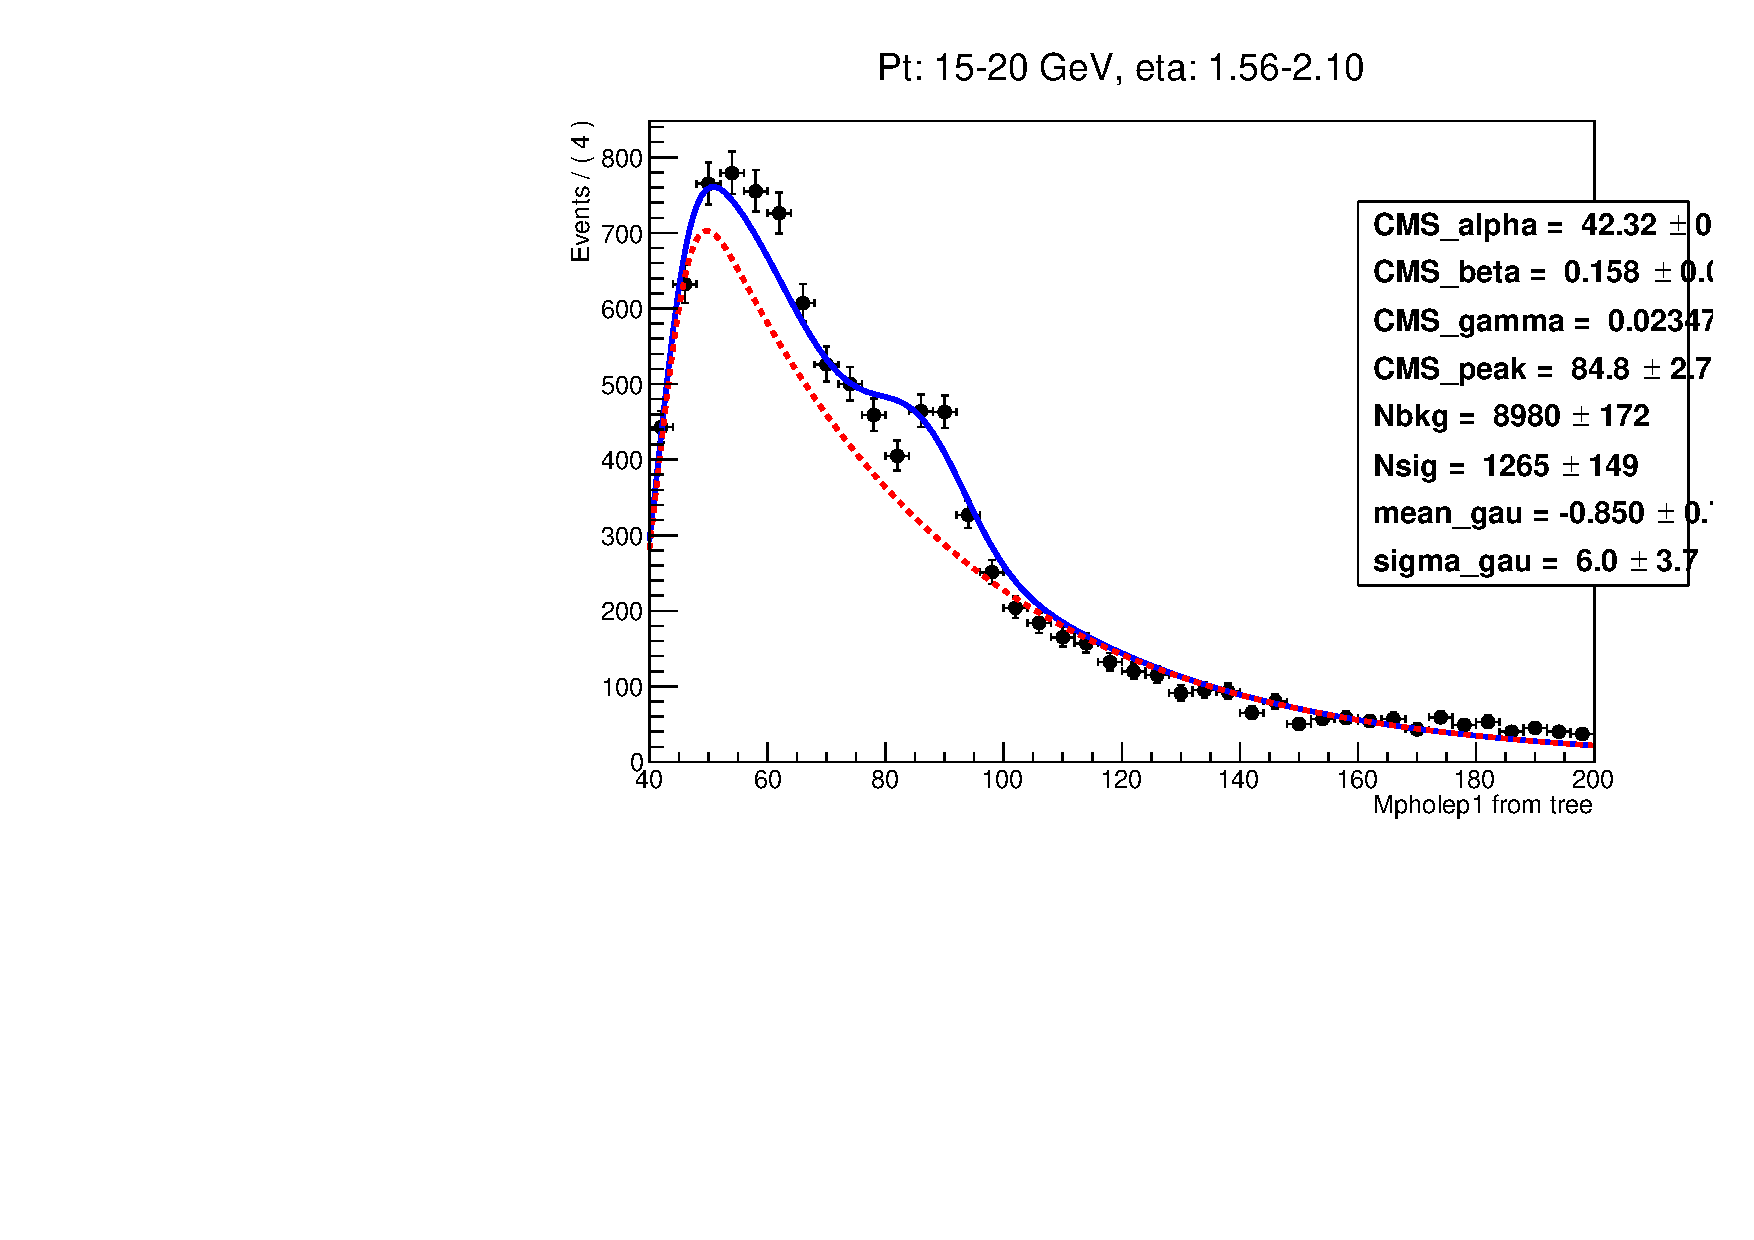
\includegraphics[width=0.45\textwidth]{../figs/figs_v11/ELECTRON_WGamma/EtoGammaFits/sa_hZmass_h_Data_EtoGamma_Enr_ENDCAP_pt15to20_ieta0.pdf}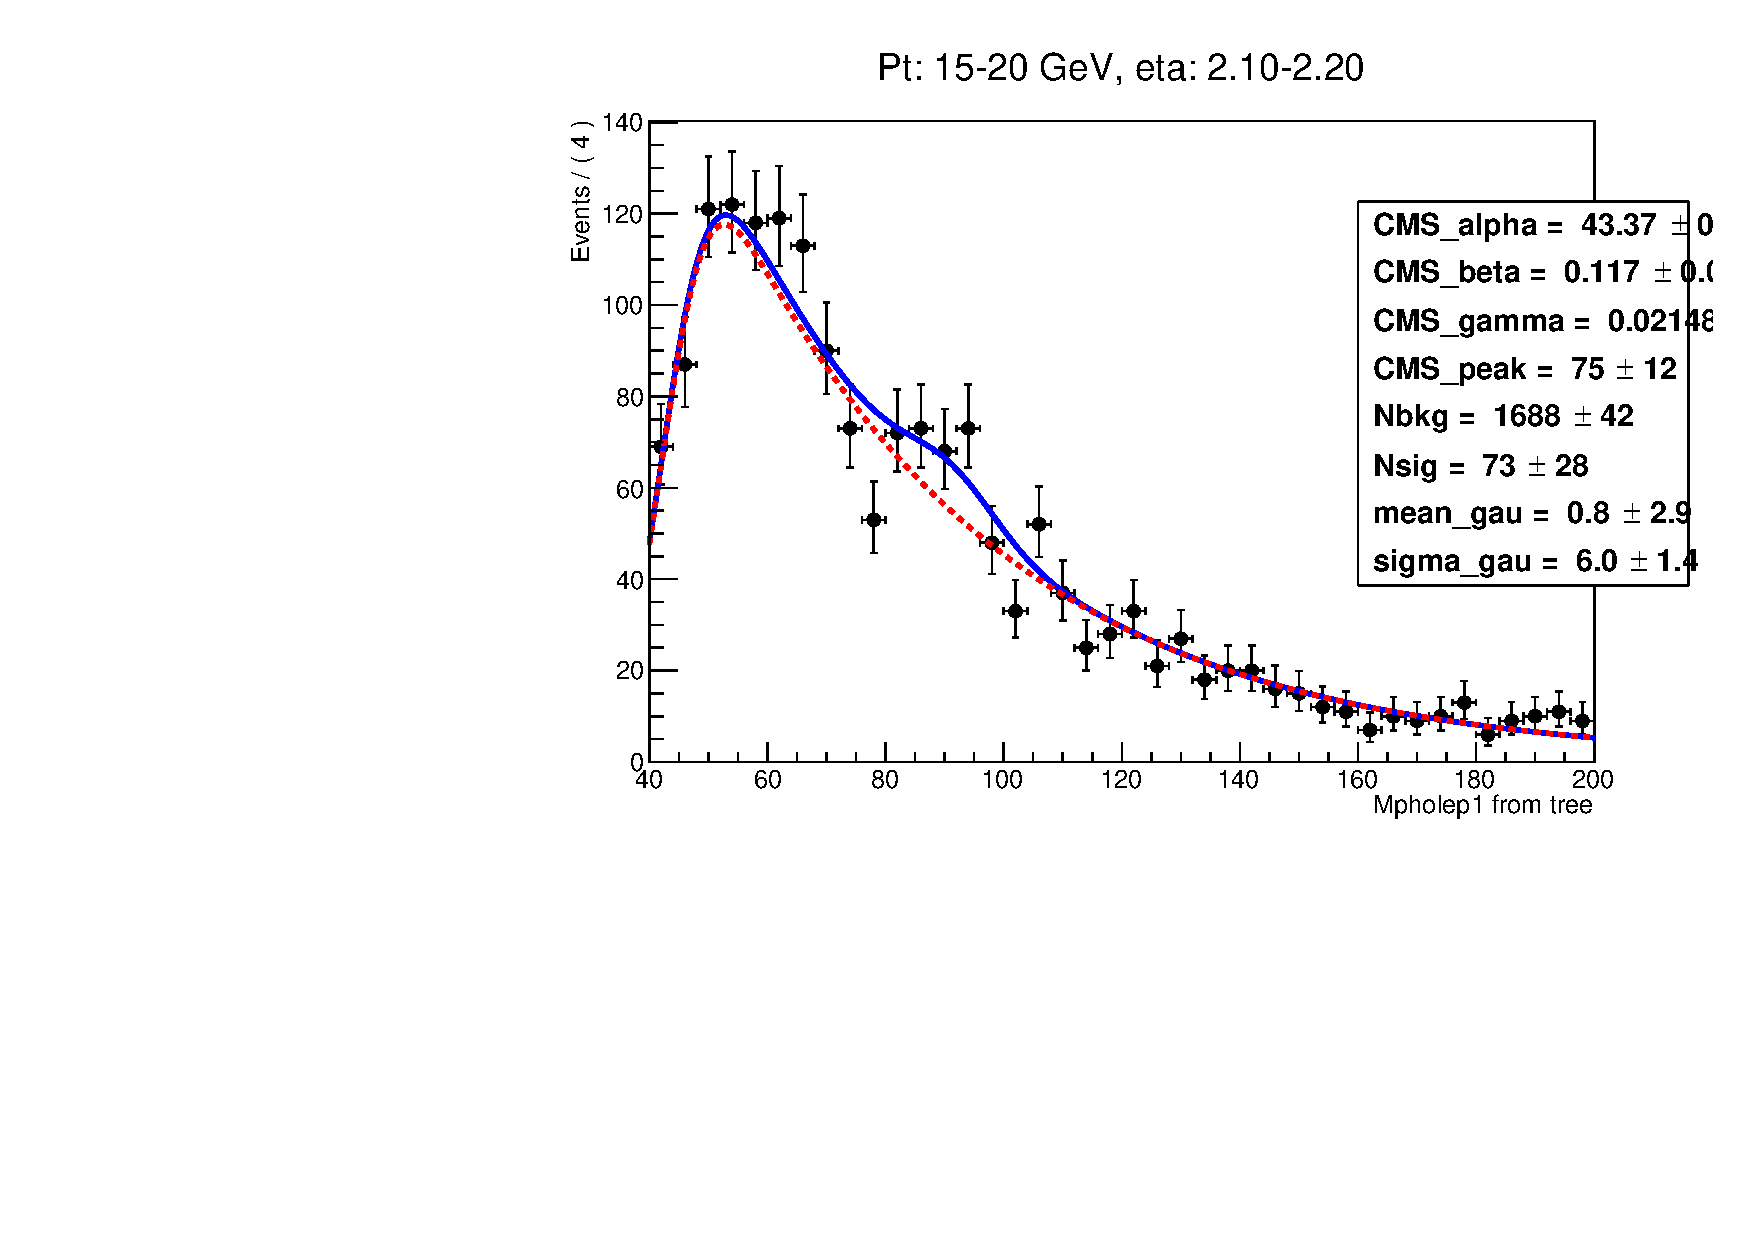
\includegraphics[width=0.45\textwidth]{../figs/figs_v11/ELECTRON_WGamma/EtoGammaFits/sa_hZmass_h_Data_EtoGamma_Enr_ENDCAP_pt15to20_ieta1.pdf}\\
   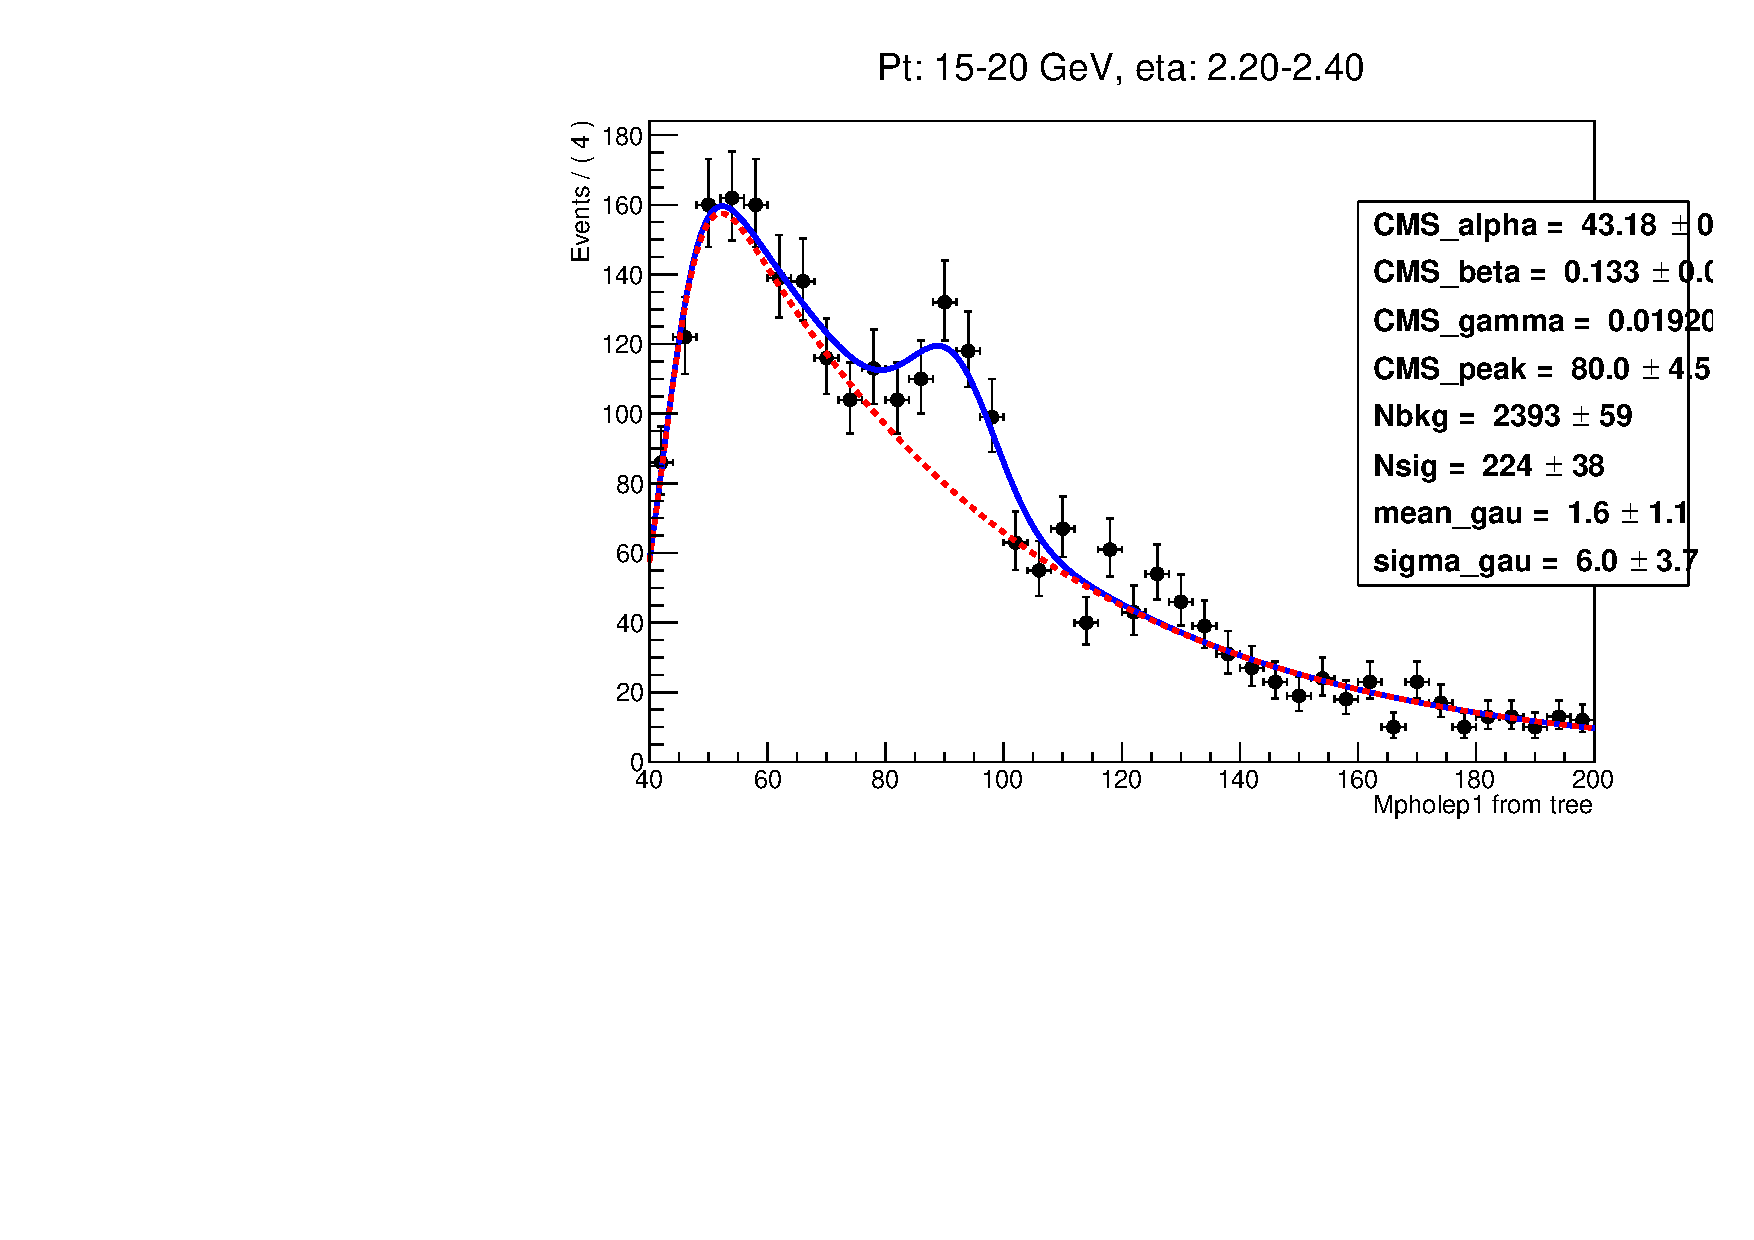
\includegraphics[width=0.45\textwidth]{../figs/figs_v11/ELECTRON_WGamma/EtoGammaFits/sa_hZmass_h_Data_EtoGamma_Enr_ENDCAP_pt15to20_ieta2.pdf}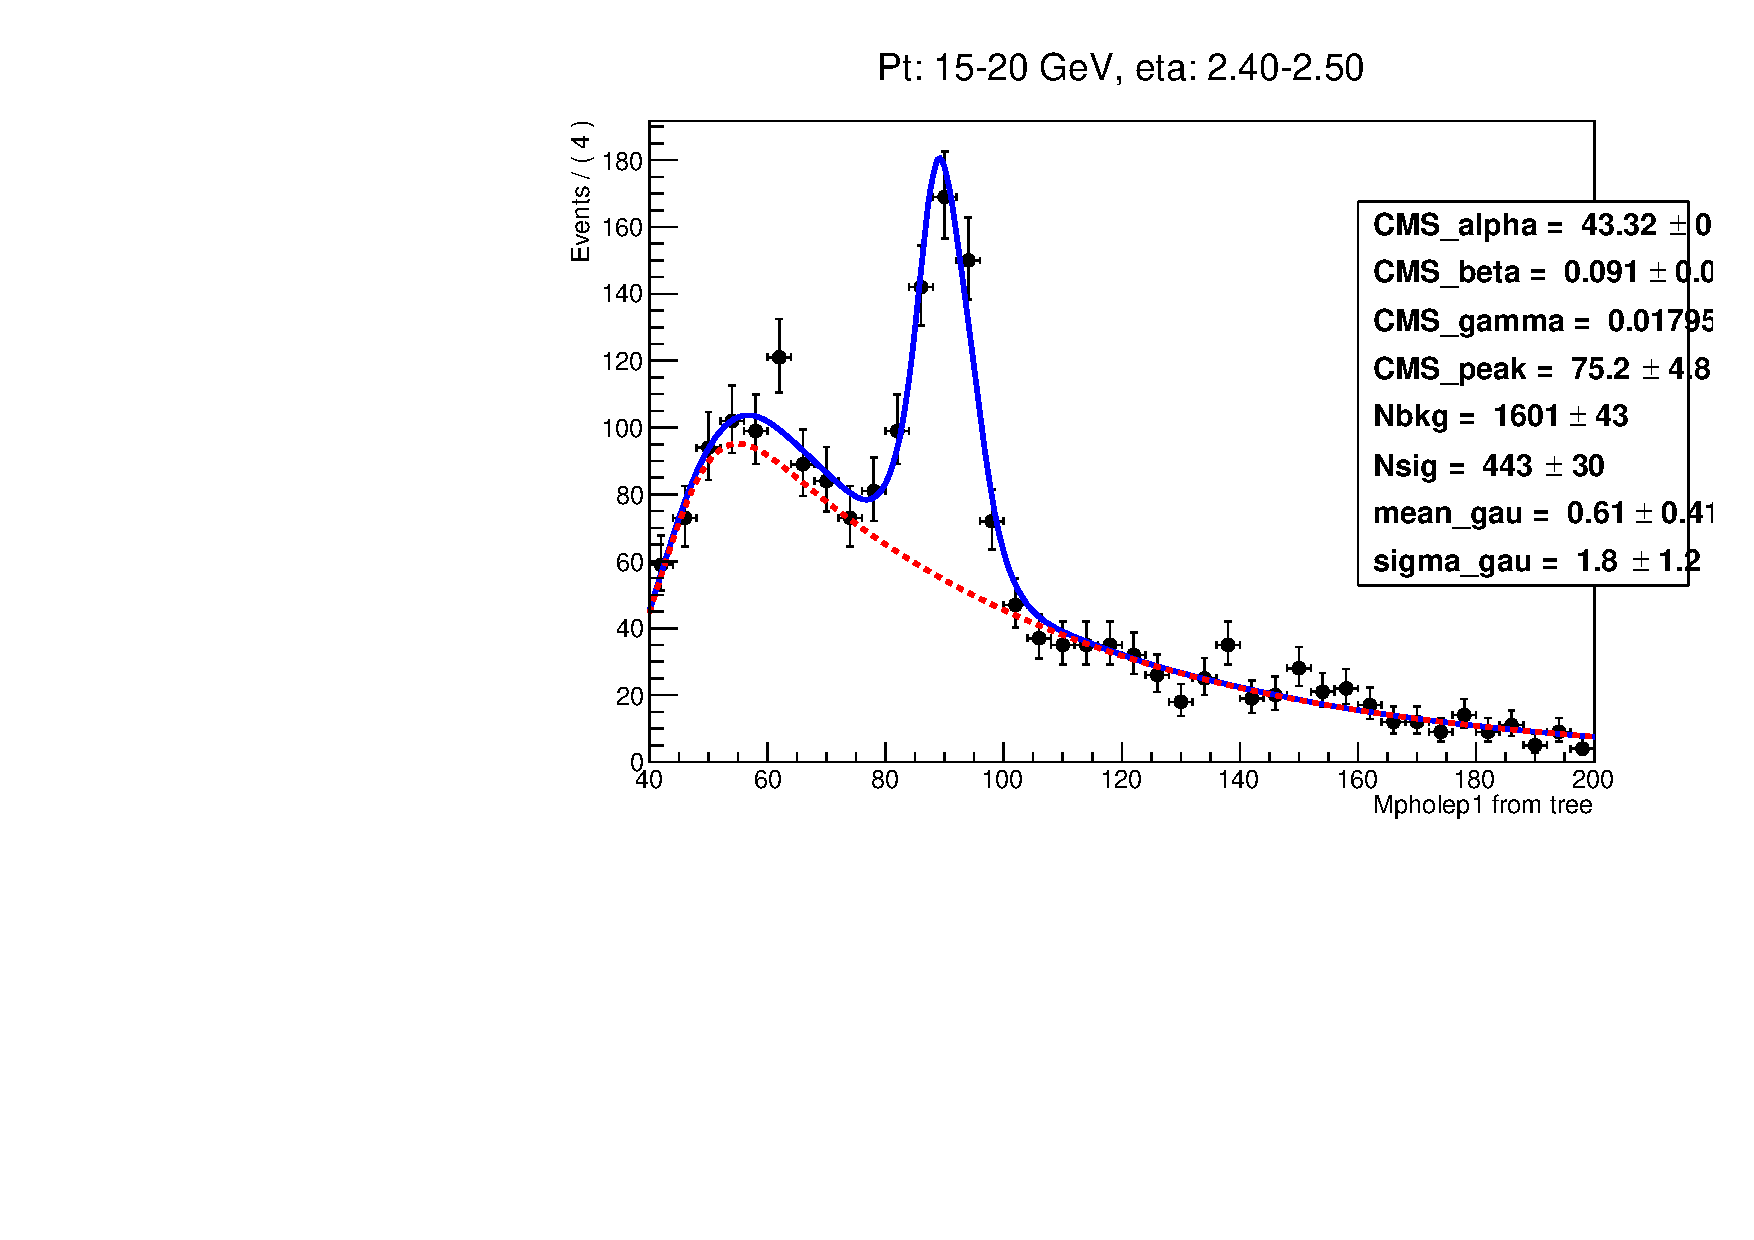
\includegraphics[width=0.45\textwidth]{../figs/figs_v11/ELECTRON_WGamma/EtoGammaFits/sa_hZmass_h_Data_EtoGamma_Enr_ENDCAP_pt15to20_ieta3.pdf}\\
  \label{fig:etogFits_15to20}
  \caption{$M_{e,\gamma}$ fits, W$\gamma$, electron channel, underflow bin (15-20 GeV), 8 eta bins}
  \end{center}
\end{figure}

\begin{figure}[htb]
  \begin{center}
   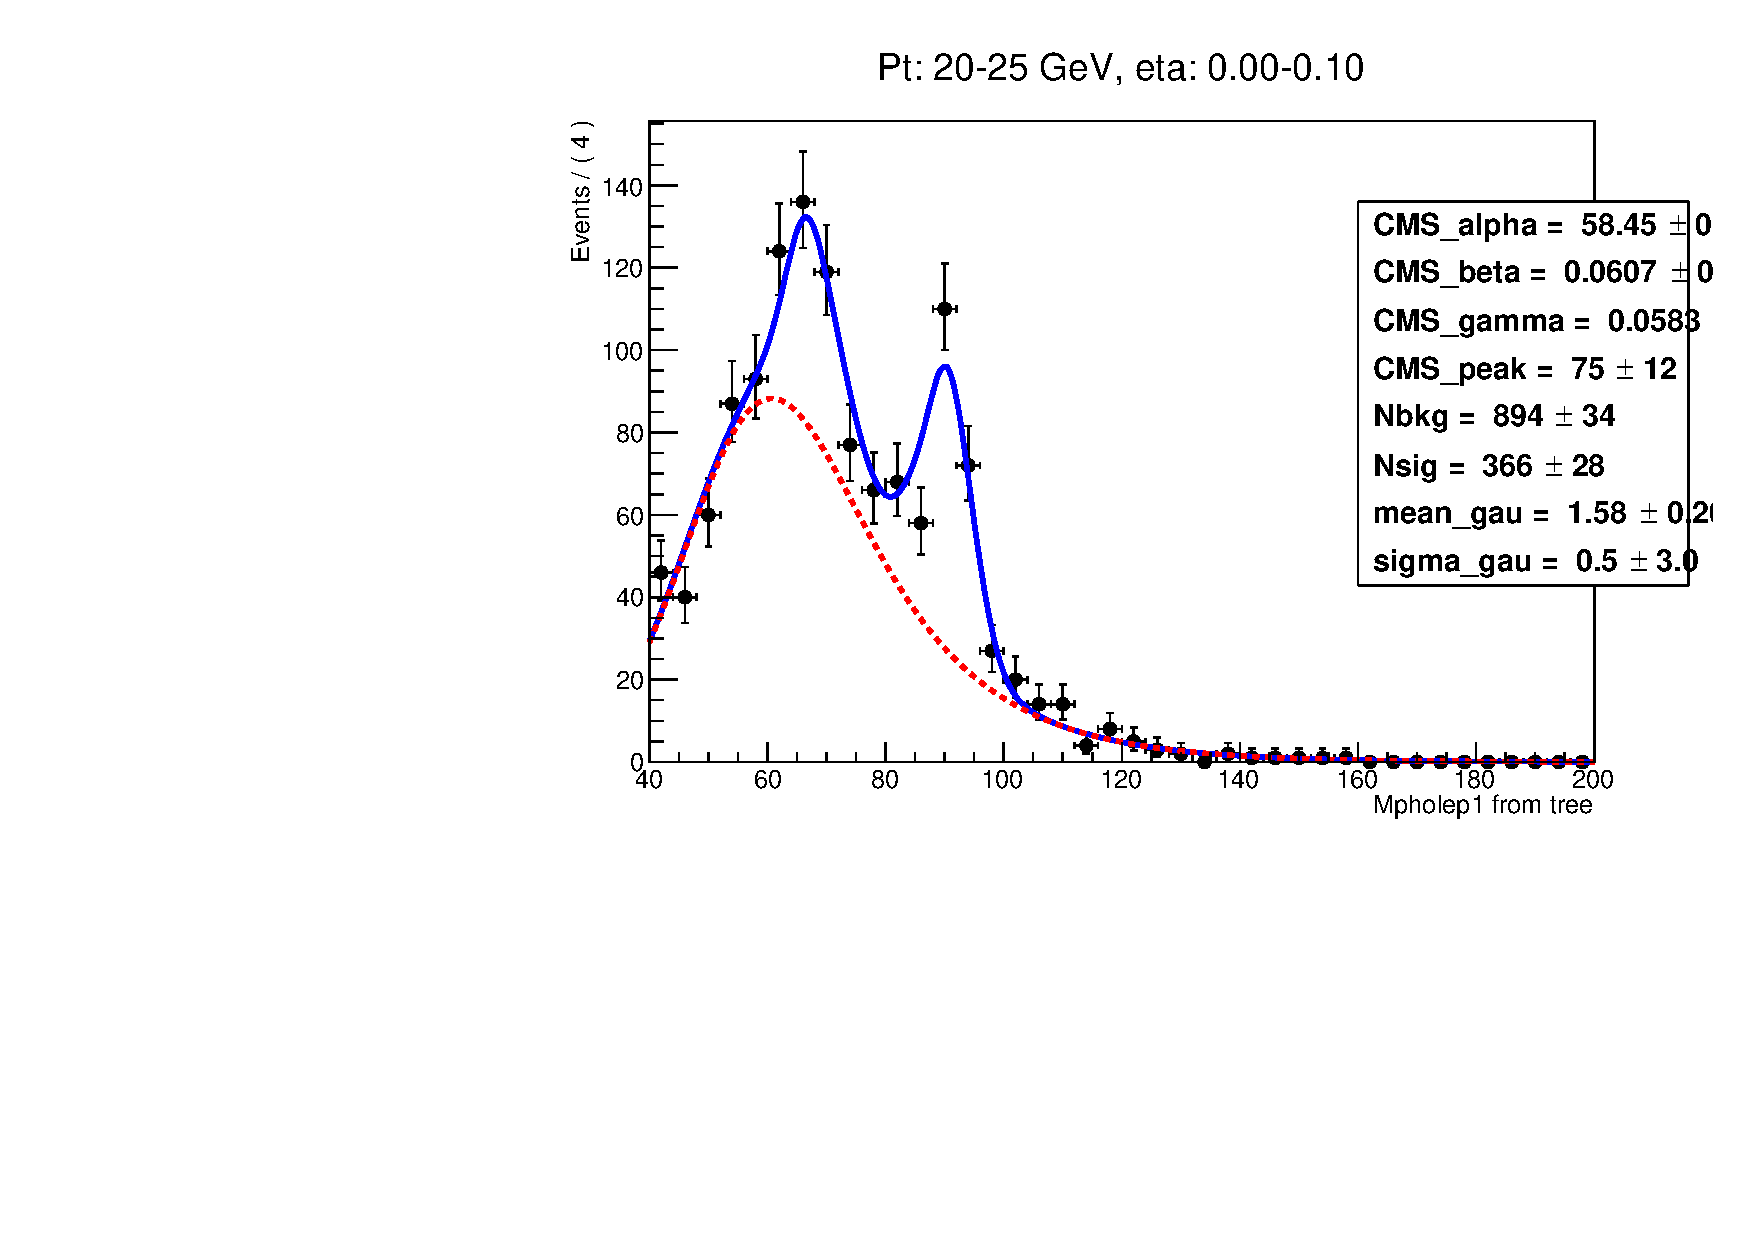
\includegraphics[width=0.45\textwidth]{../figs/figs_v11/ELECTRON_WGamma/EtoGammaFits/sa_hZmass_h_Data_EtoGamma_Enr_BARREL_pt20to25_ieta0.pdf}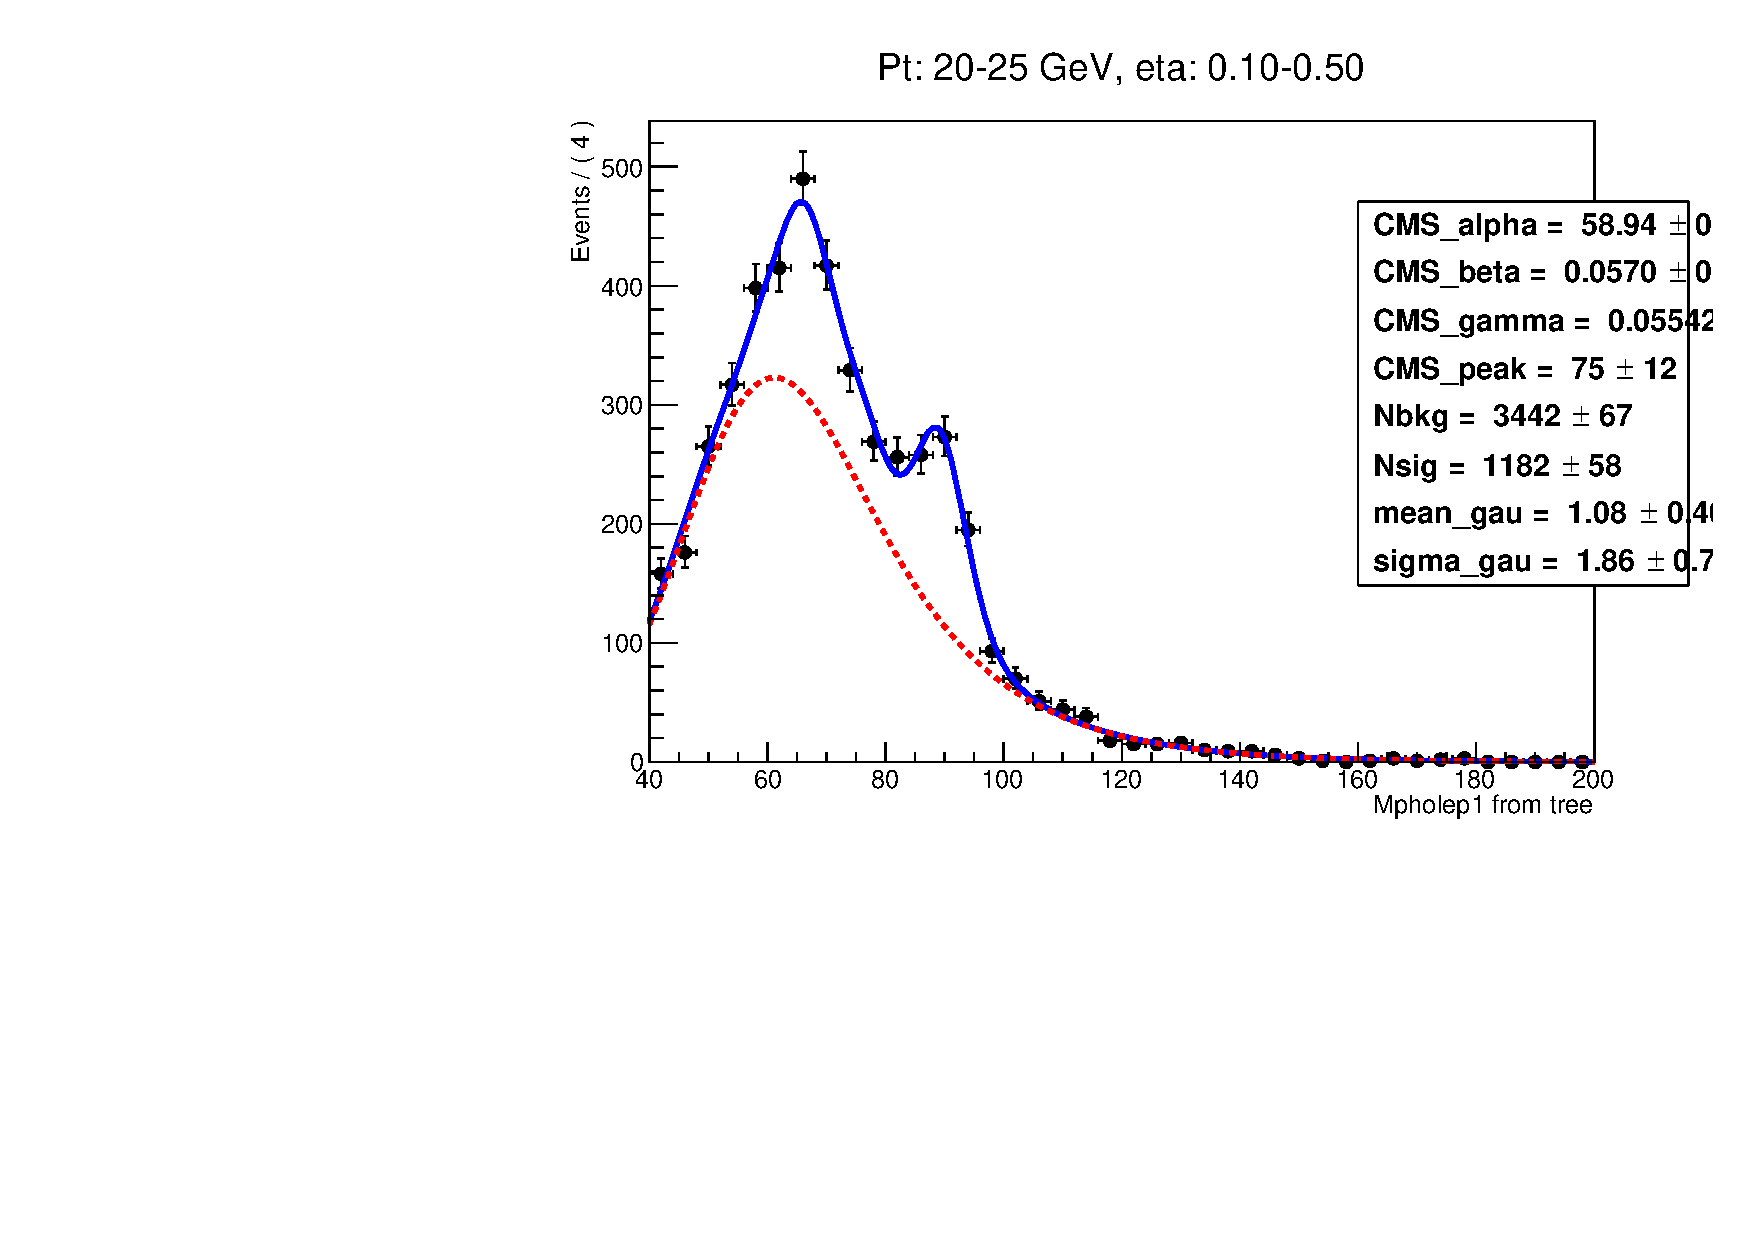
\includegraphics[width=0.45\textwidth]{../figs/figs_v11/ELECTRON_WGamma/EtoGammaFits/sa_hZmass_h_Data_EtoGamma_Enr_BARREL_pt20to25_ieta1.pdf}\\
   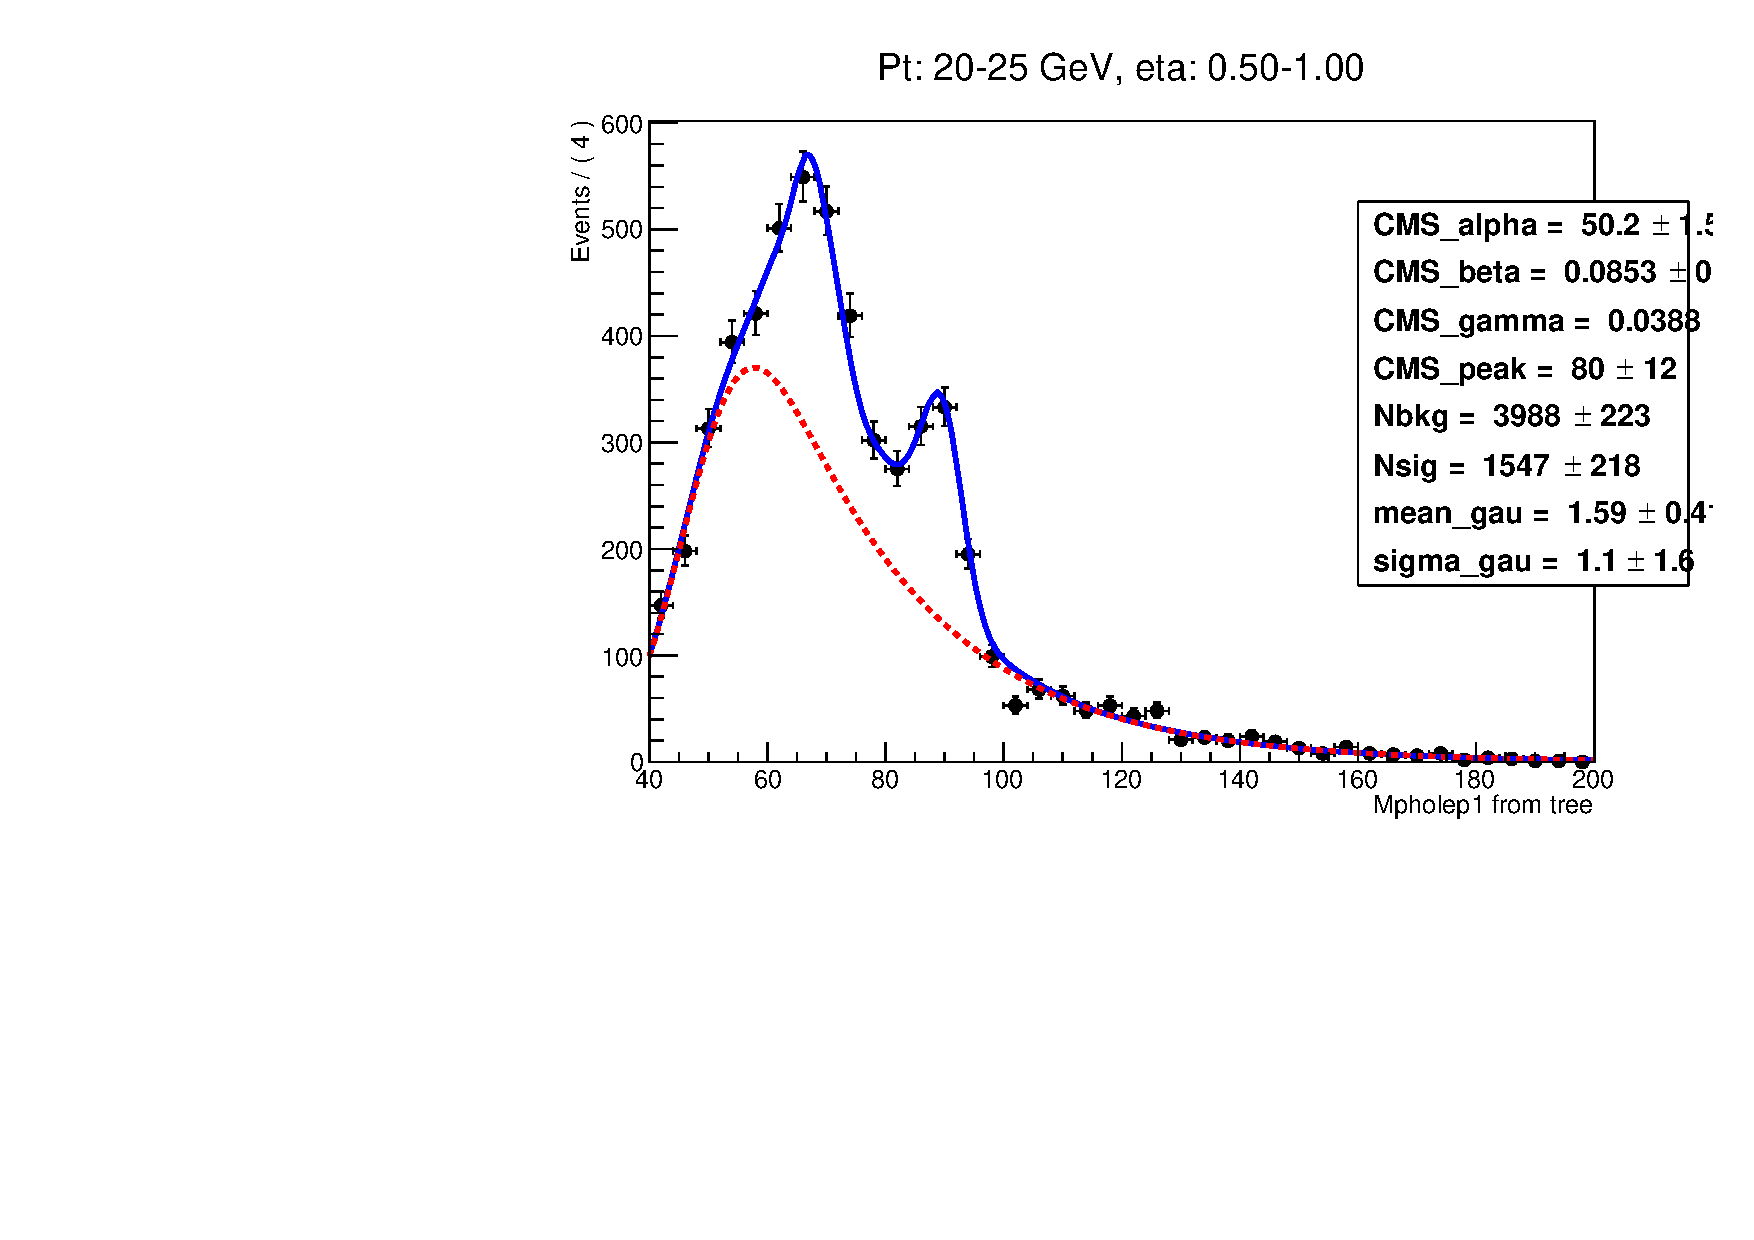
\includegraphics[width=0.45\textwidth]{../figs/figs_v11/ELECTRON_WGamma/EtoGammaFits/sa_hZmass_h_Data_EtoGamma_Enr_BARREL_pt20to25_ieta2.pdf}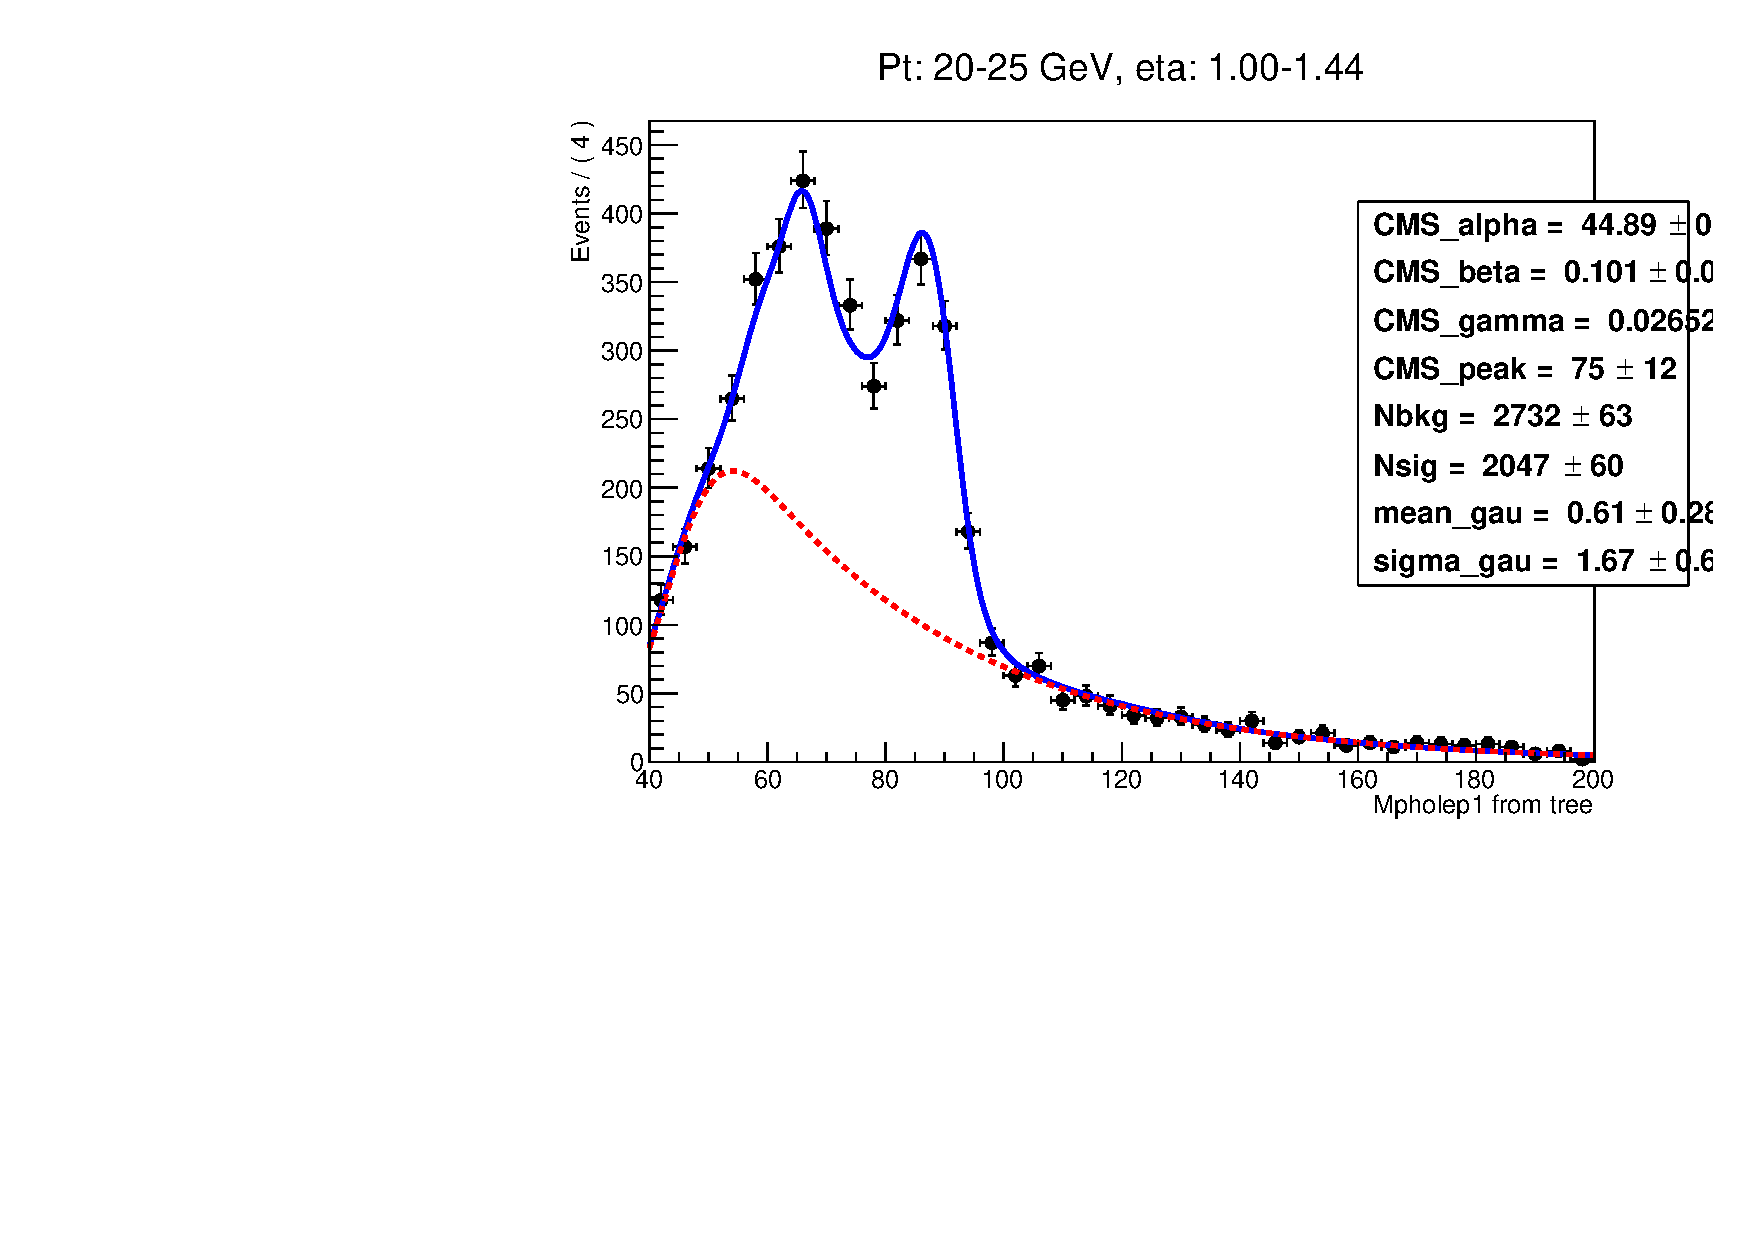
\includegraphics[width=0.45\textwidth]{../figs/figs_v11/ELECTRON_WGamma/EtoGammaFits/sa_hZmass_h_Data_EtoGamma_Enr_BARREL_pt20to25_ieta3.pdf}\\
   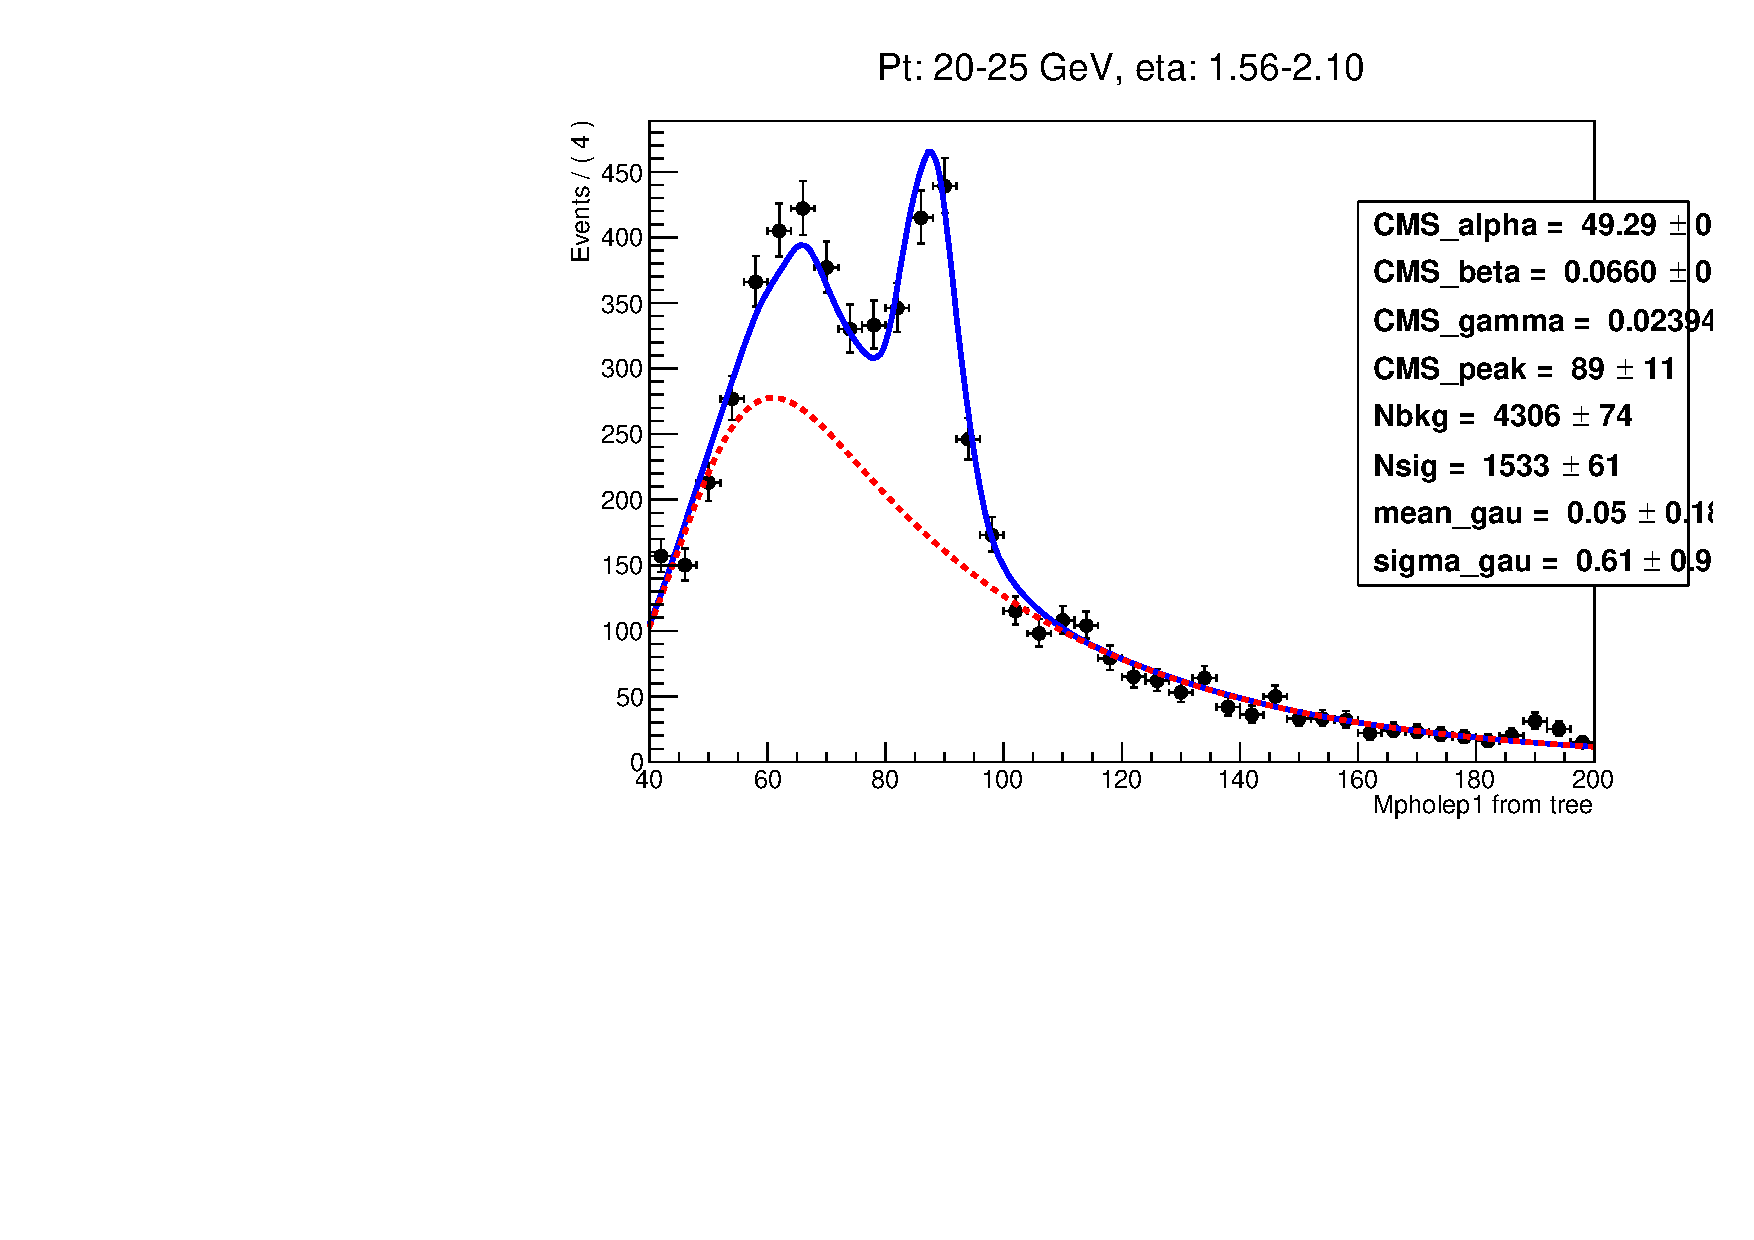
\includegraphics[width=0.45\textwidth]{../figs/figs_v11/ELECTRON_WGamma/EtoGammaFits/sa_hZmass_h_Data_EtoGamma_Enr_ENDCAP_pt20to25_ieta0.pdf}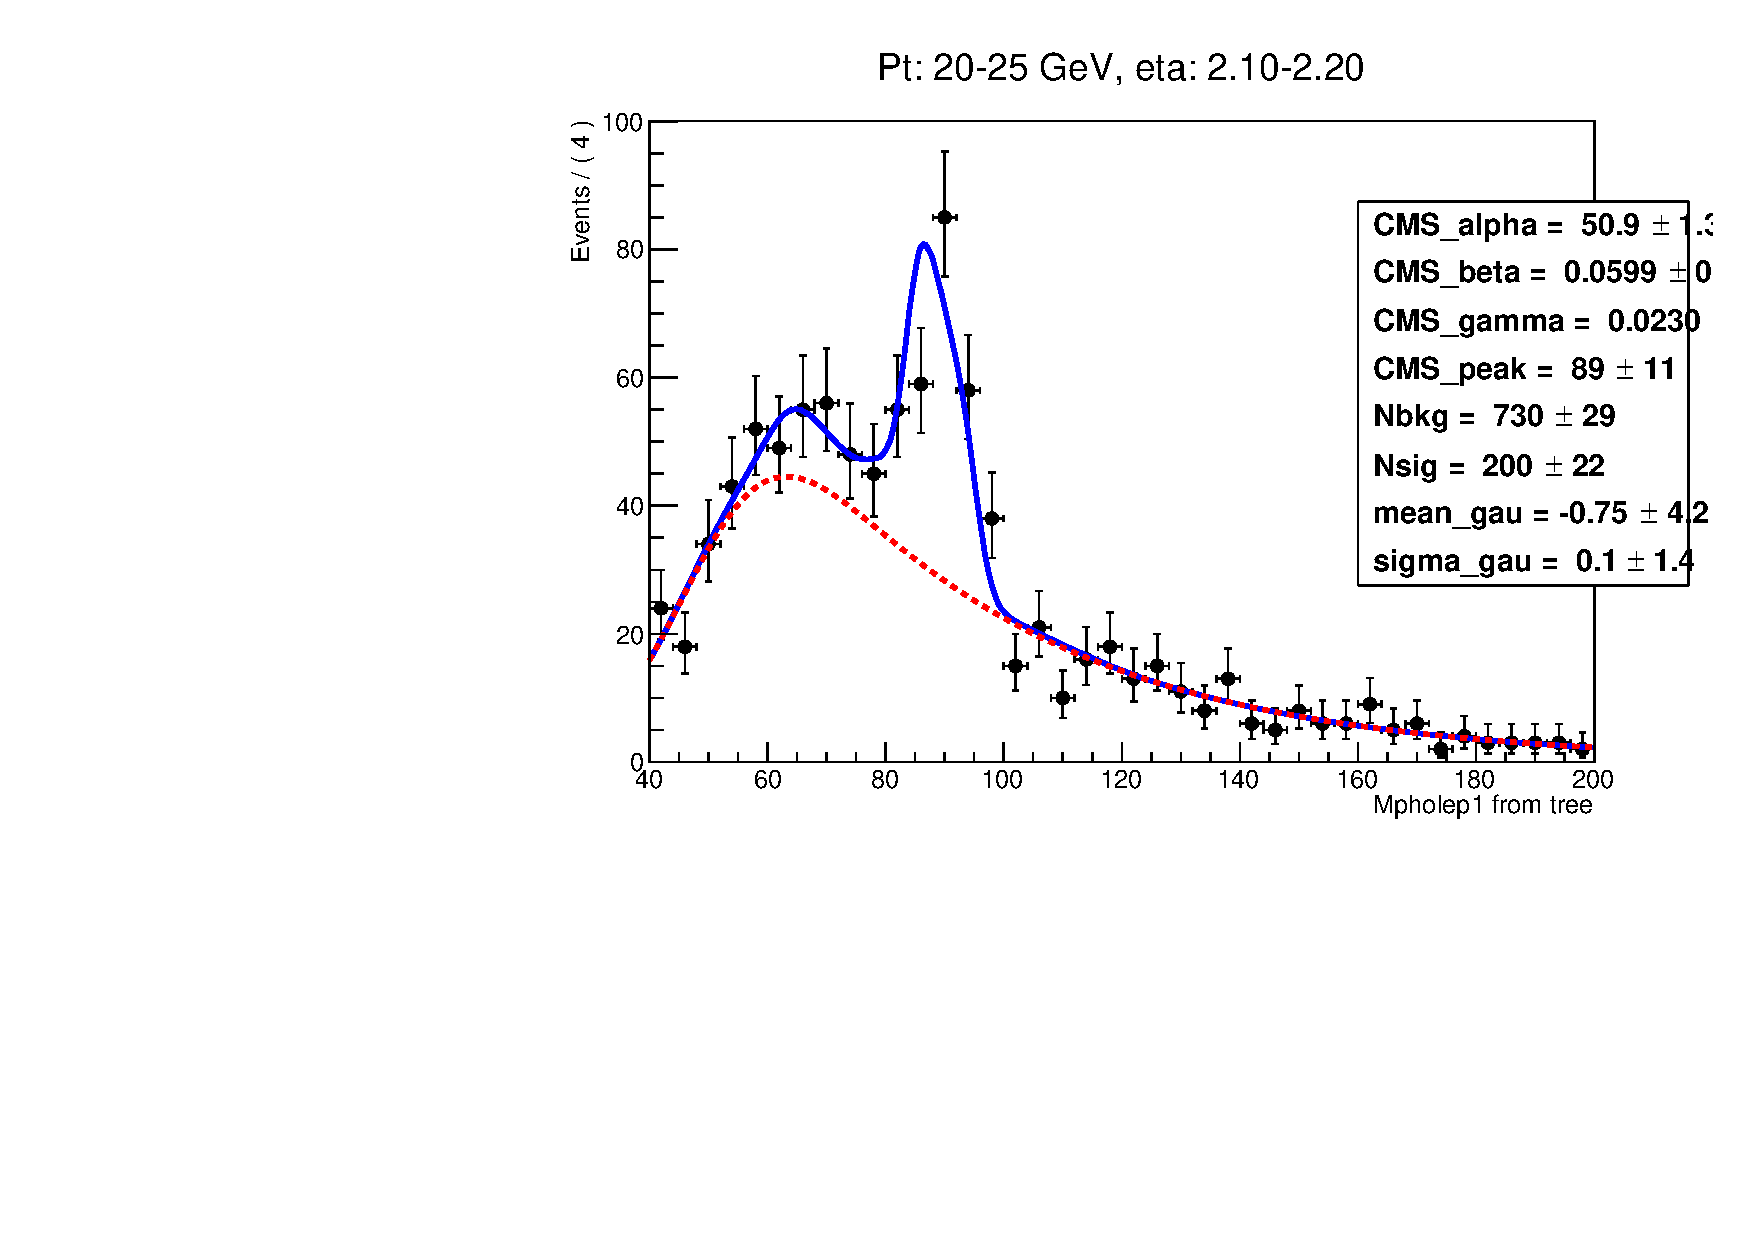
\includegraphics[width=0.45\textwidth]{../figs/figs_v11/ELECTRON_WGamma/EtoGammaFits/sa_hZmass_h_Data_EtoGamma_Enr_ENDCAP_pt20to25_ieta1.pdf}\\
   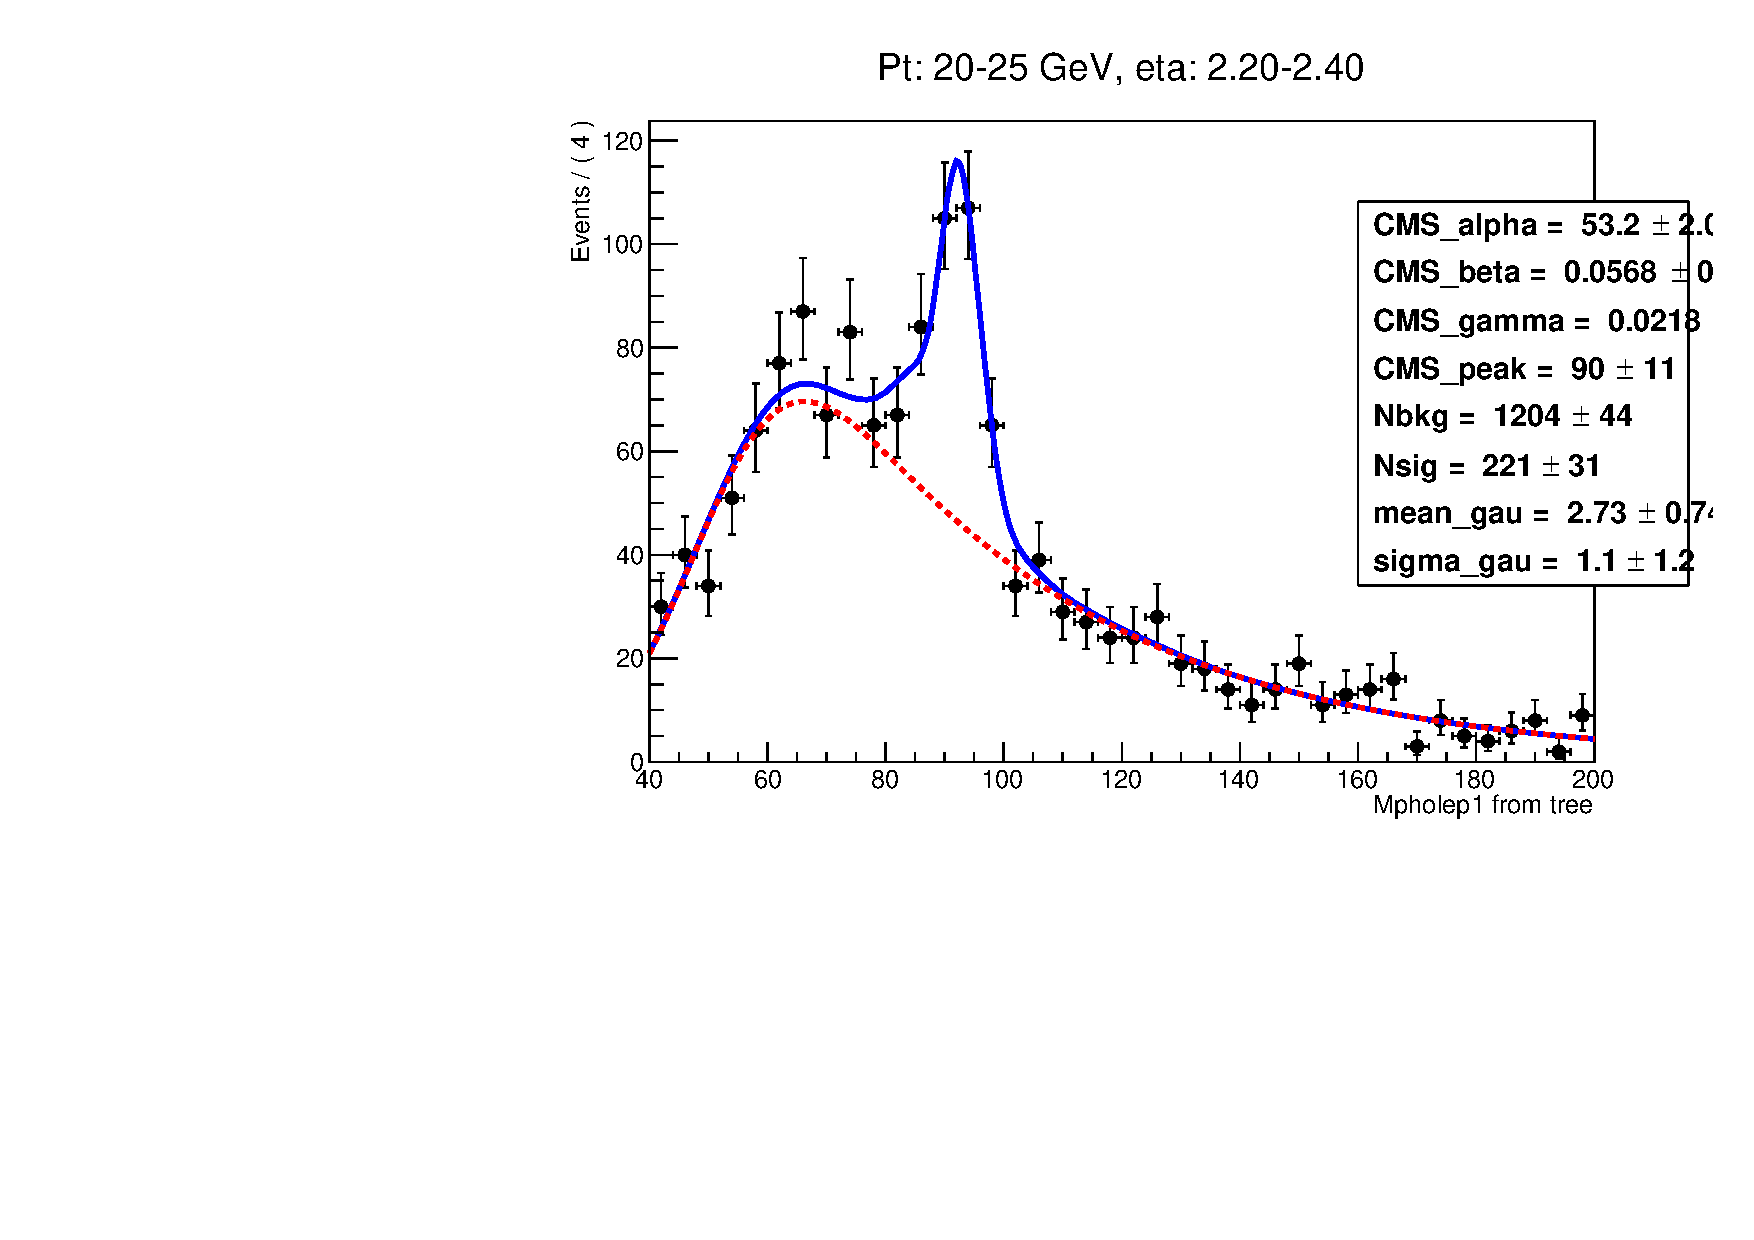
\includegraphics[width=0.45\textwidth]{../figs/figs_v11/ELECTRON_WGamma/EtoGammaFits/sa_hZmass_h_Data_EtoGamma_Enr_ENDCAP_pt20to25_ieta2.pdf}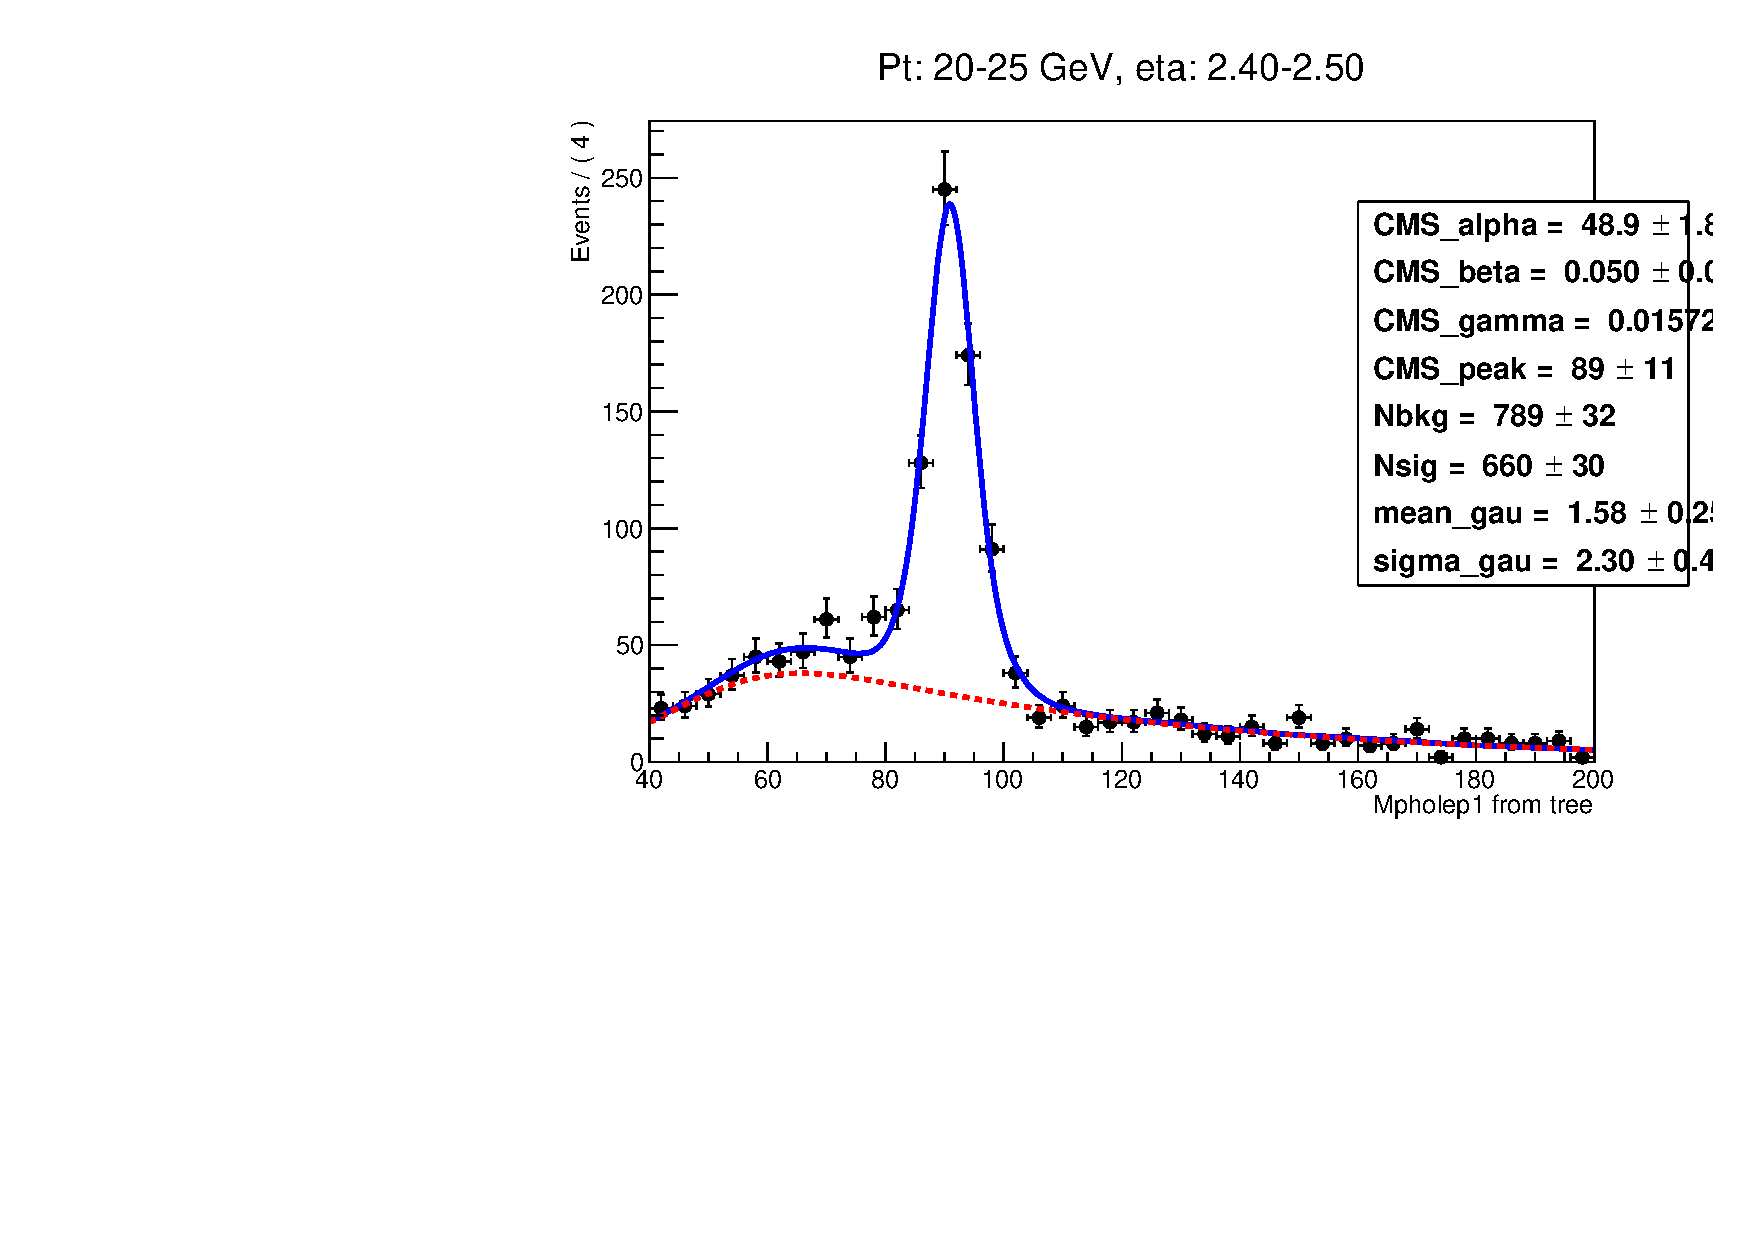
\includegraphics[width=0.45\textwidth]{../figs/figs_v11/ELECTRON_WGamma/EtoGammaFits/sa_hZmass_h_Data_EtoGamma_Enr_ENDCAP_pt20to25_ieta3.pdf}\\
  \label{fig:etogFits_20to25}
  \caption{$M_{e,\gamma}$ fits, W$\gamma$, electron channel, underflow bin (20-25 GeV), 8 eta bins}
  \end{center}
\end{figure}

\begin{figure}[htb]
  \begin{center}
   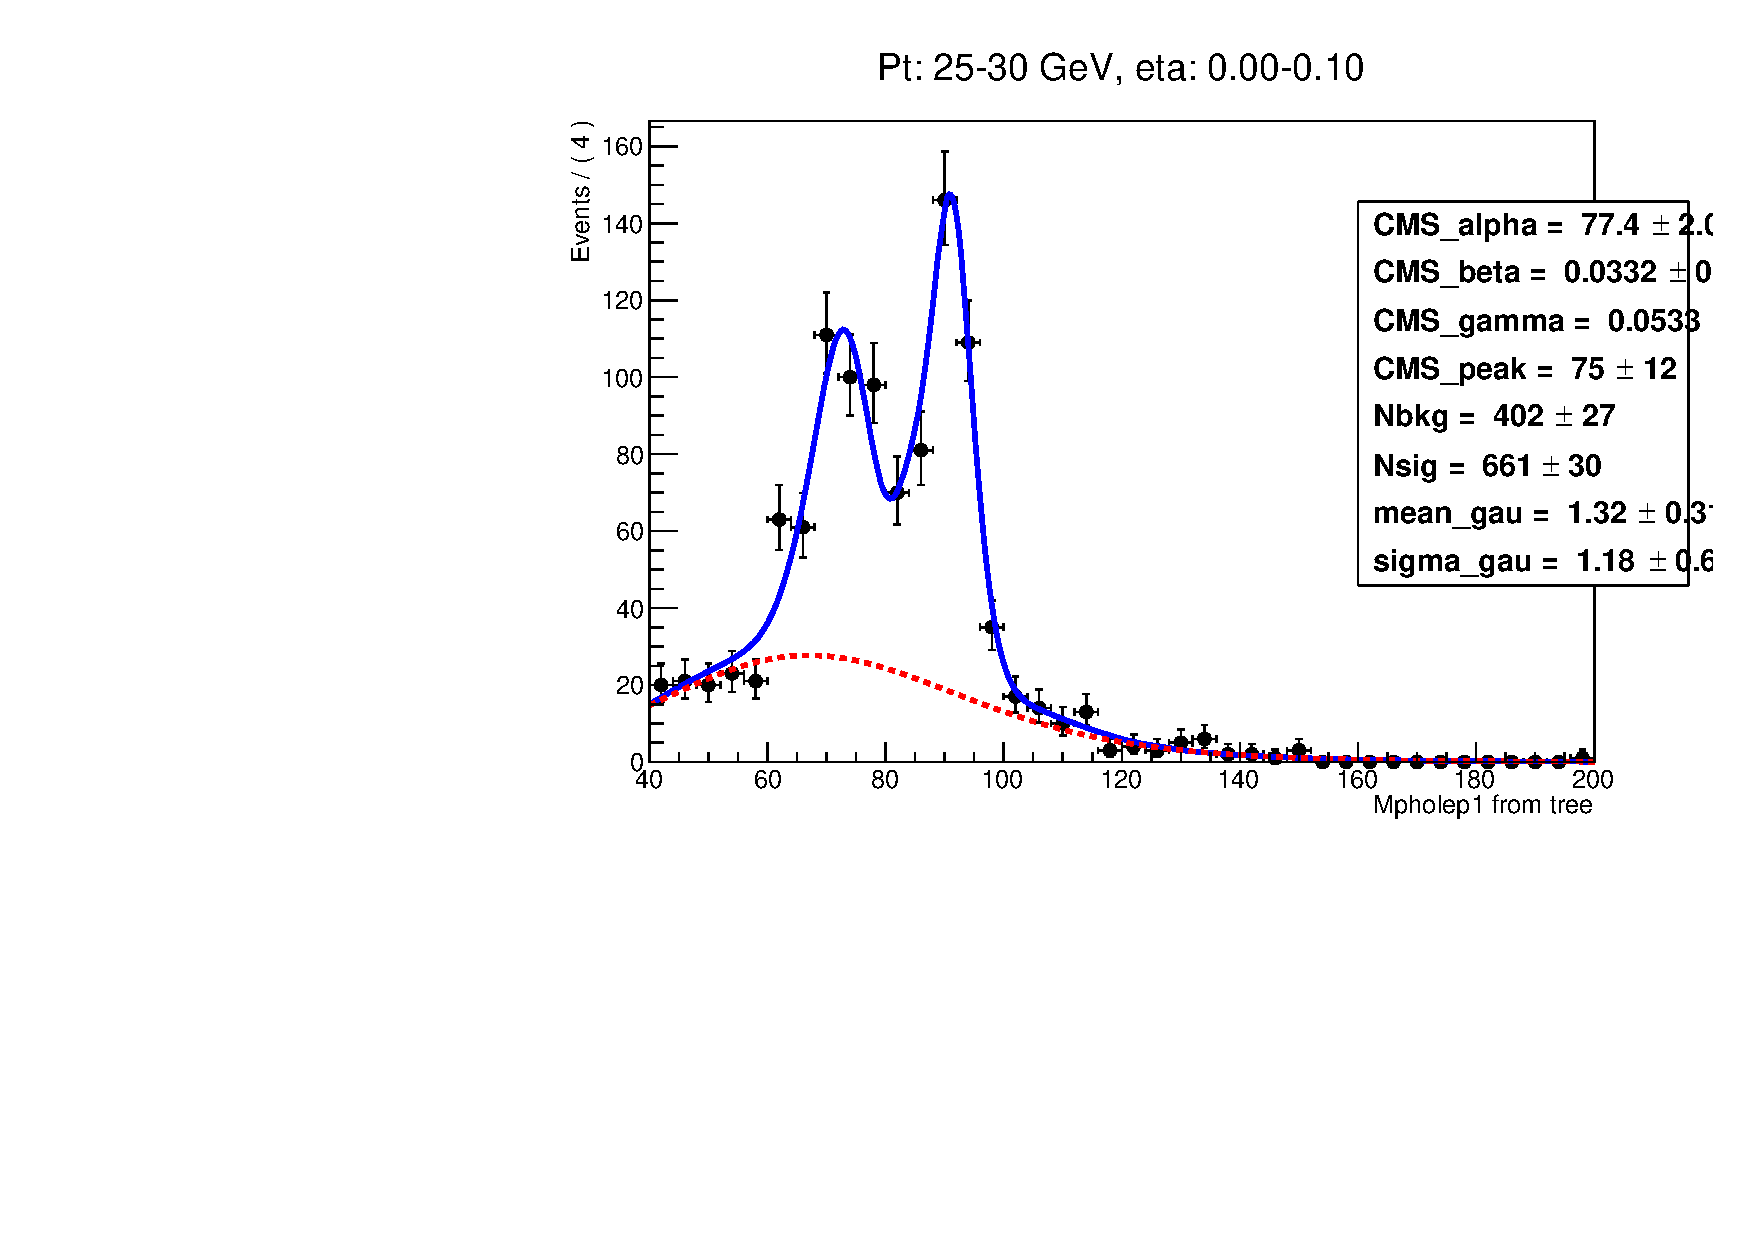
\includegraphics[width=0.45\textwidth]{../figs/figs_v11/ELECTRON_WGamma/EtoGammaFits/sa_hZmass_h_Data_EtoGamma_Enr_BARREL_pt25to30_ieta0.pdf}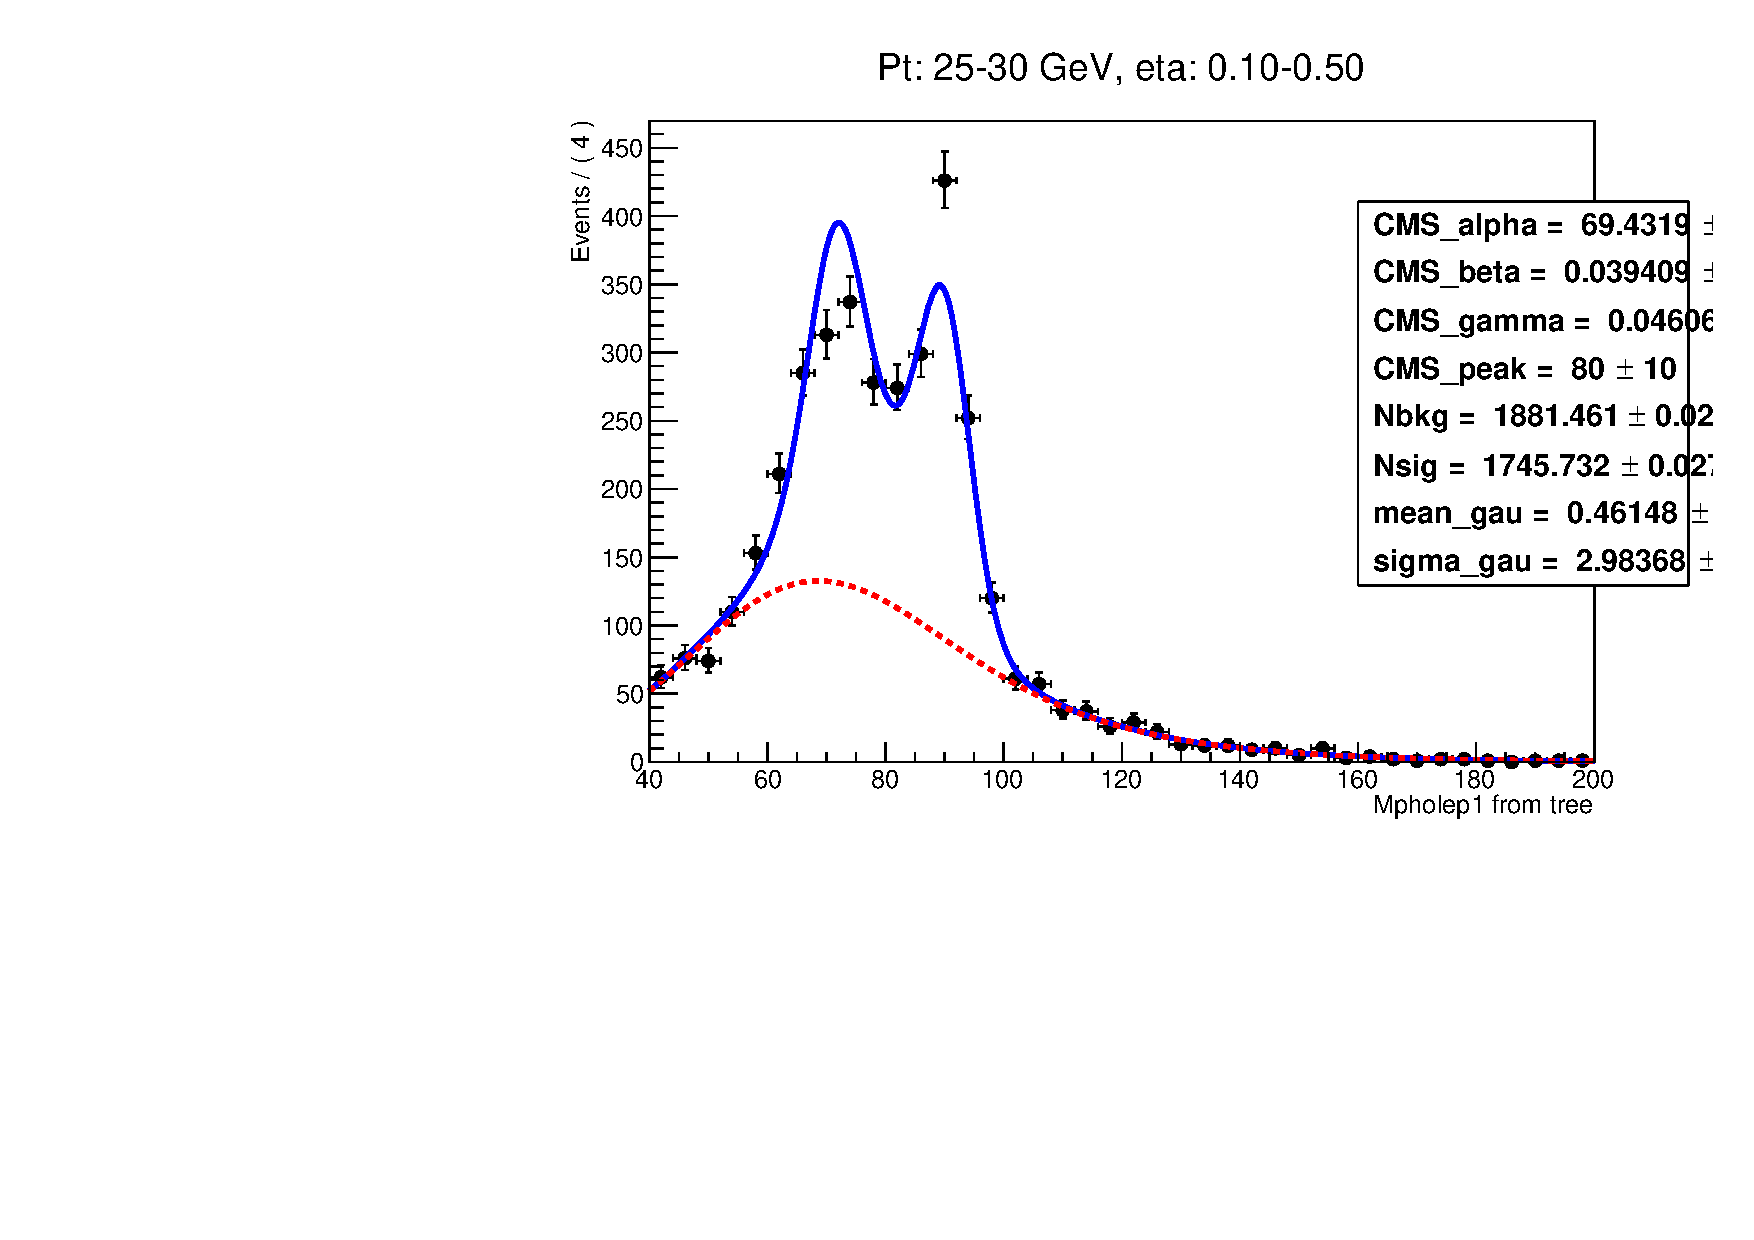
\includegraphics[width=0.45\textwidth]{../figs/figs_v11/ELECTRON_WGamma/EtoGammaFits/sa_hZmass_h_Data_EtoGamma_Enr_BARREL_pt25to30_ieta1.pdf}\\
   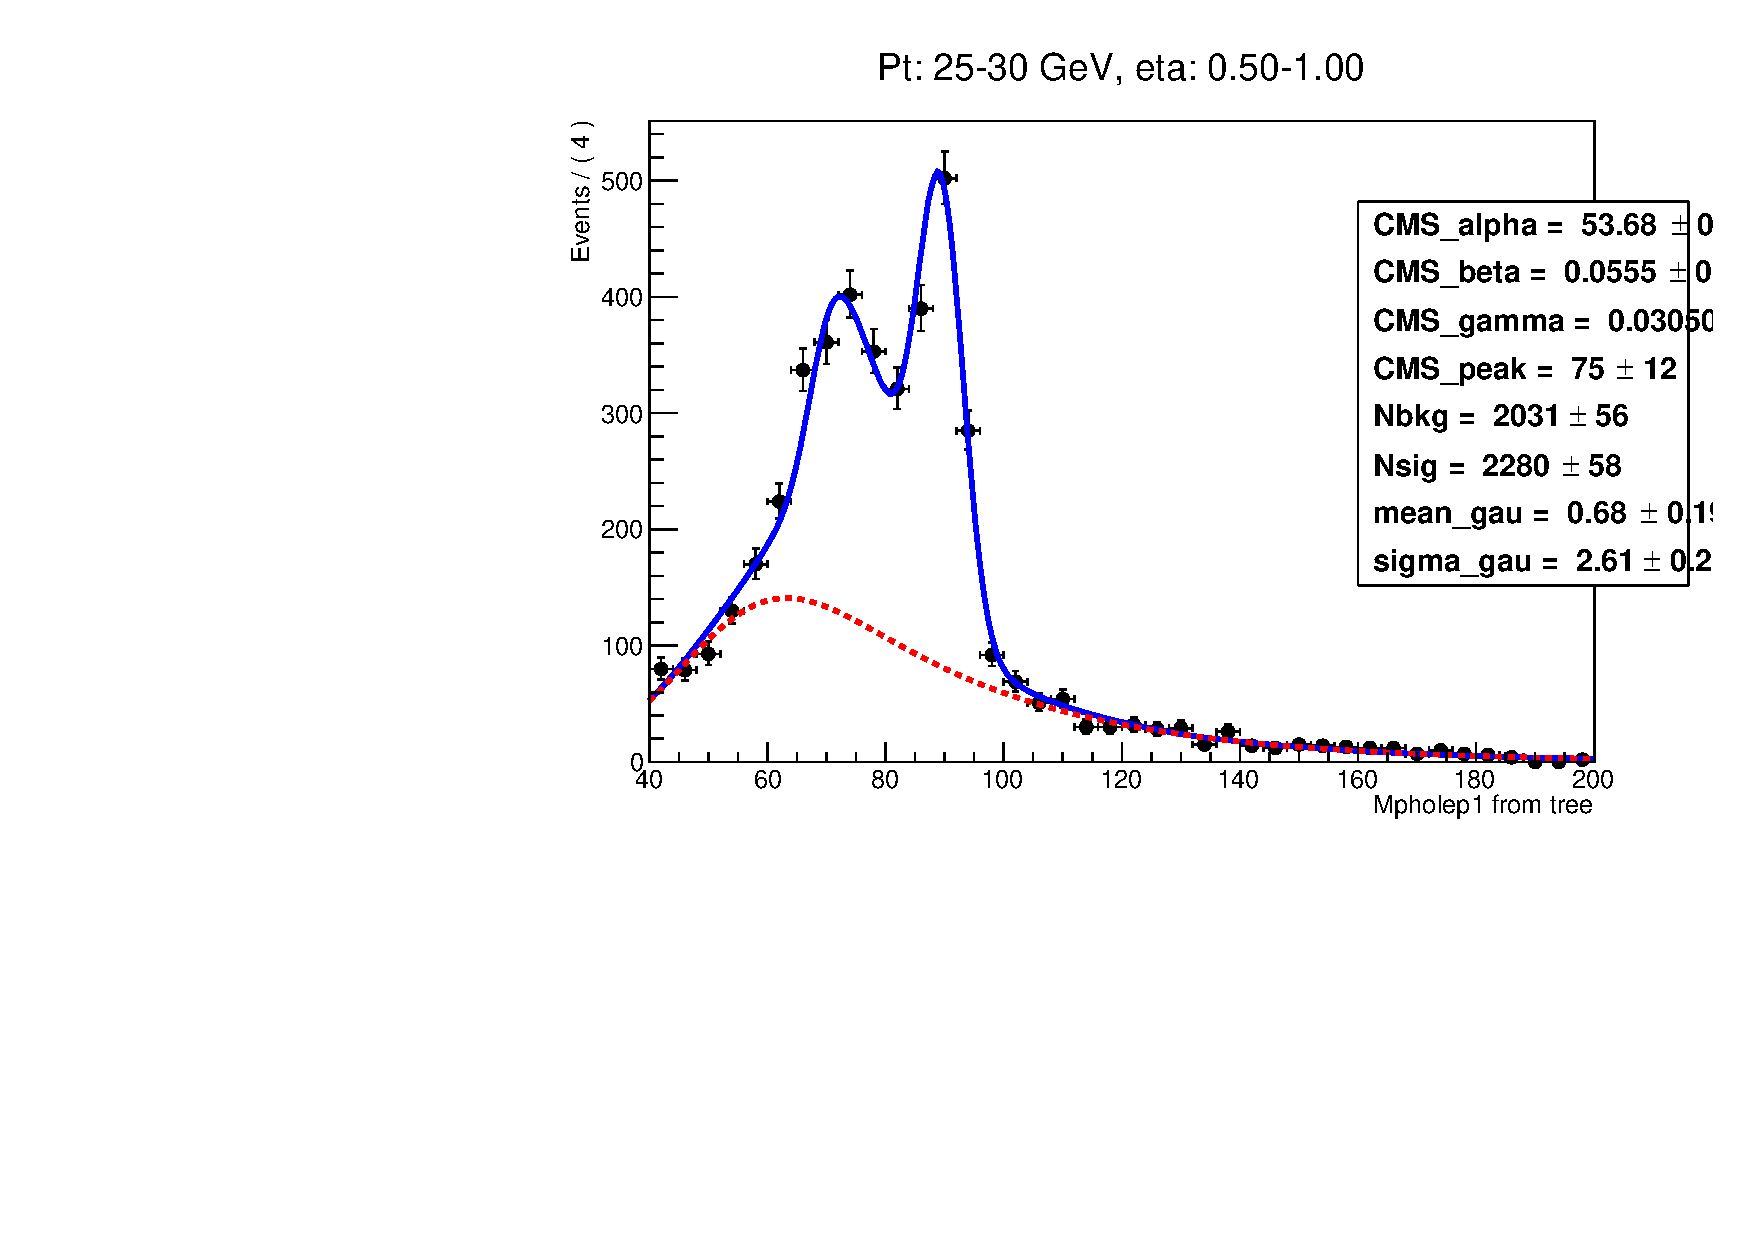
\includegraphics[width=0.45\textwidth]{../figs/figs_v11/ELECTRON_WGamma/EtoGammaFits/sa_hZmass_h_Data_EtoGamma_Enr_BARREL_pt25to30_ieta2.pdf}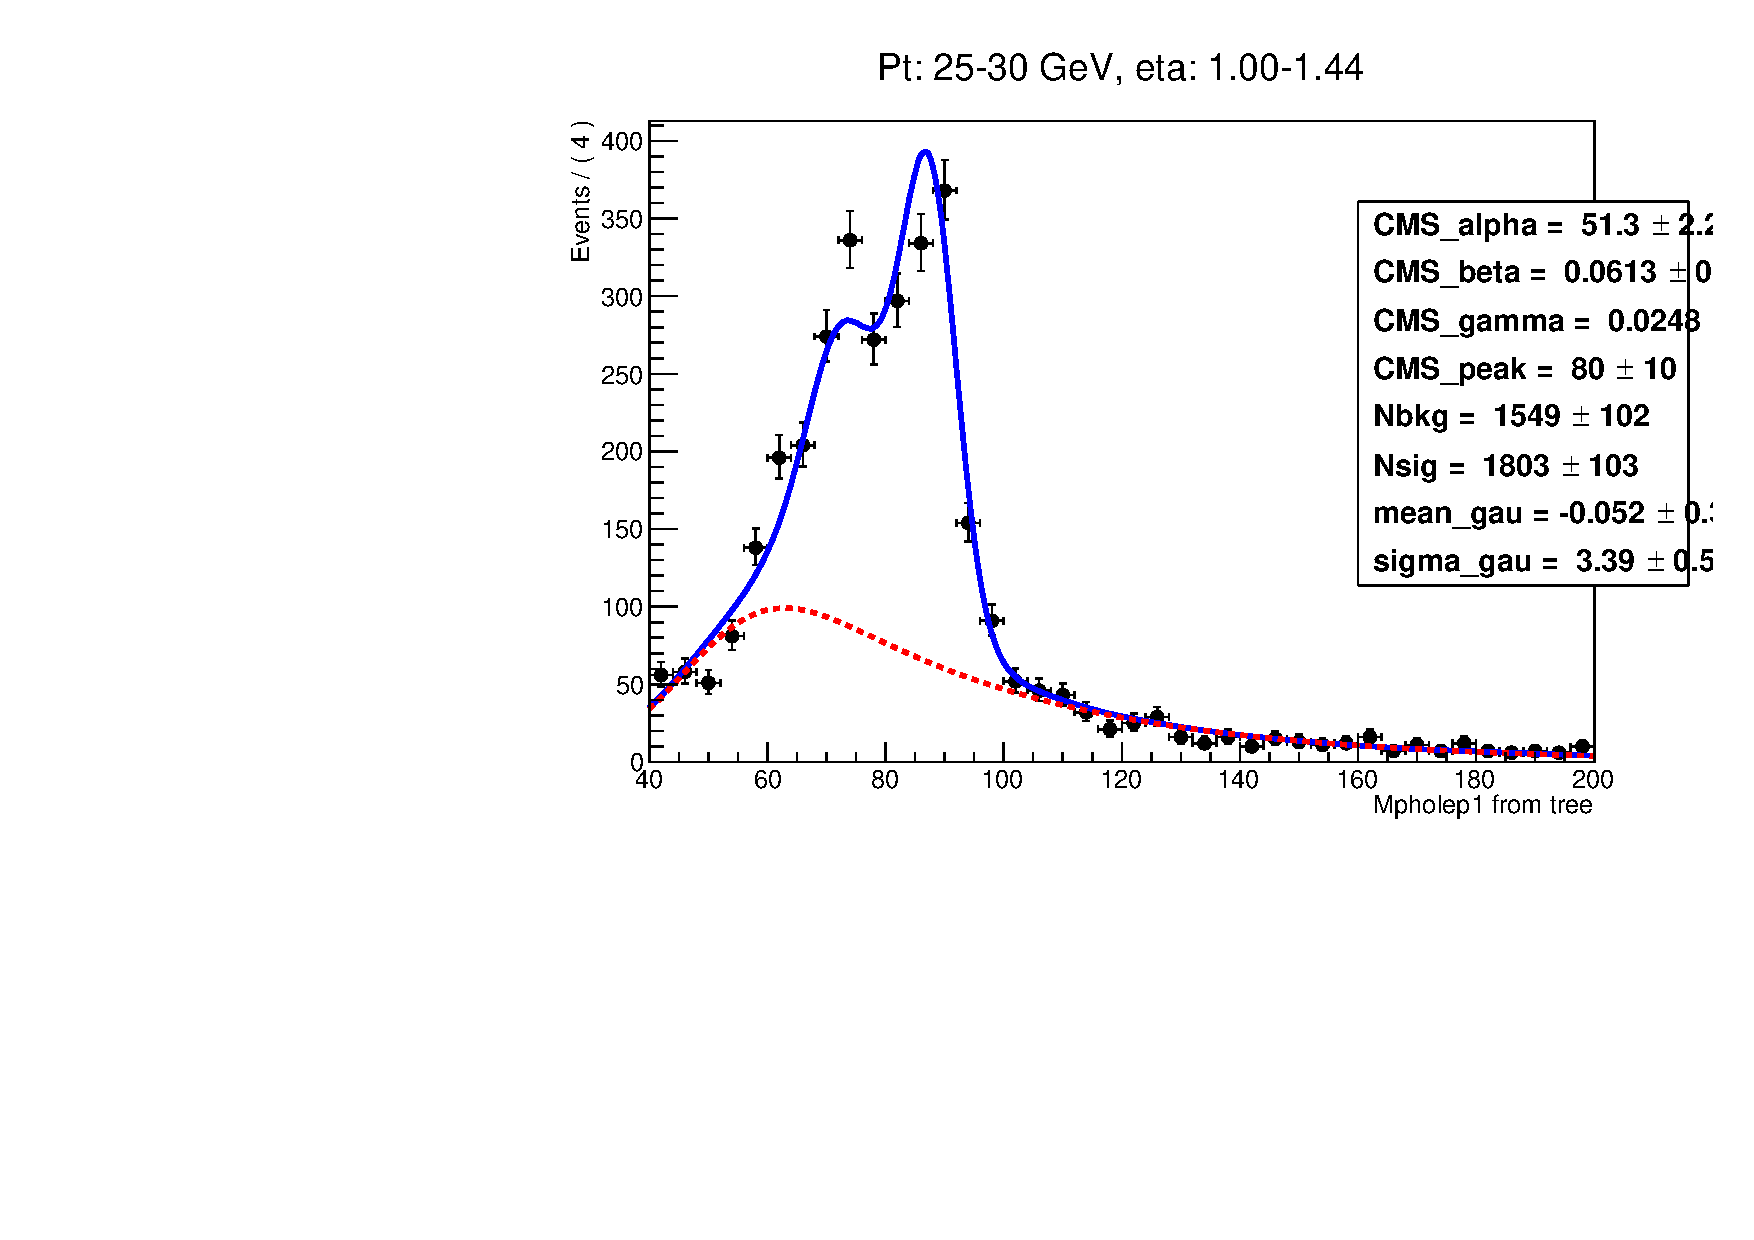
\includegraphics[width=0.45\textwidth]{../figs/figs_v11/ELECTRON_WGamma/EtoGammaFits/sa_hZmass_h_Data_EtoGamma_Enr_BARREL_pt25to30_ieta3.pdf}\\
   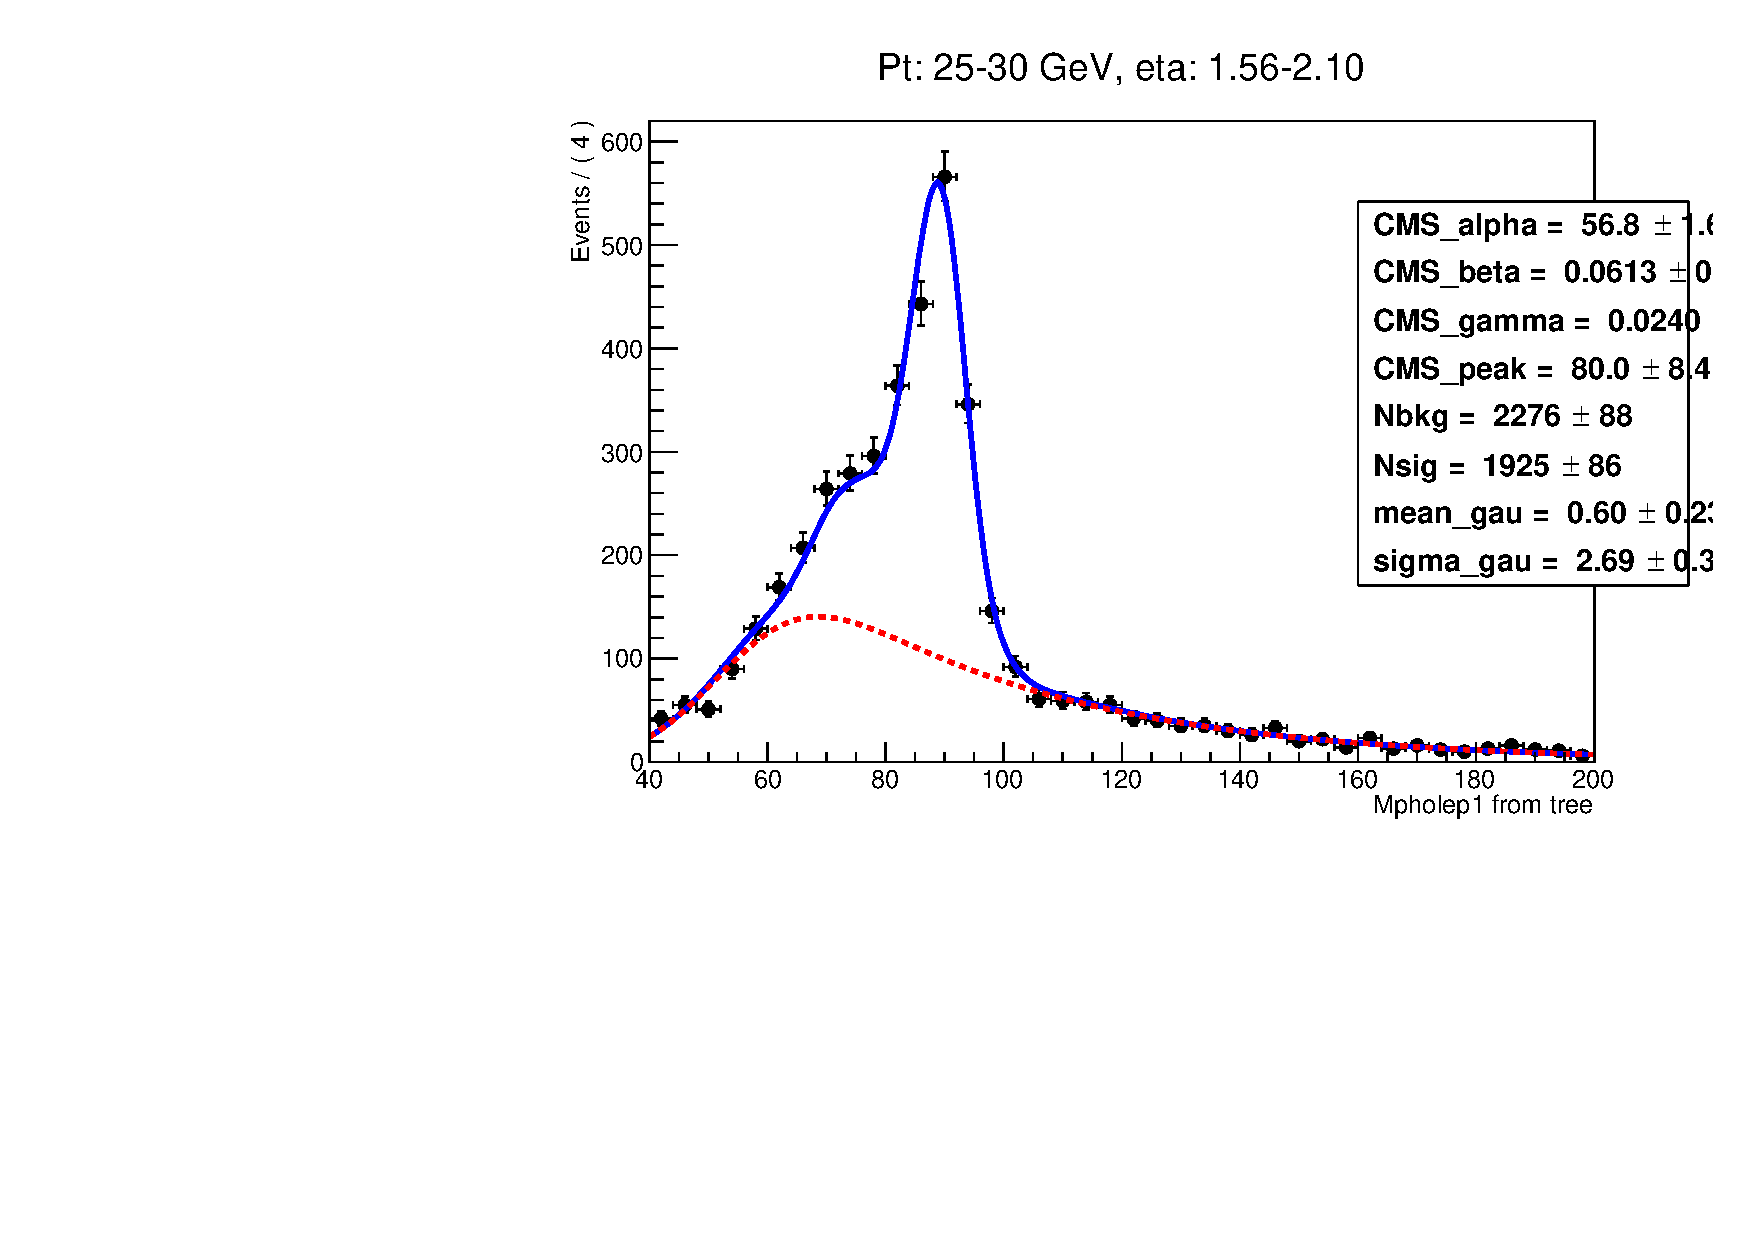
\includegraphics[width=0.45\textwidth]{../figs/figs_v11/ELECTRON_WGamma/EtoGammaFits/sa_hZmass_h_Data_EtoGamma_Enr_ENDCAP_pt25to30_ieta0.pdf}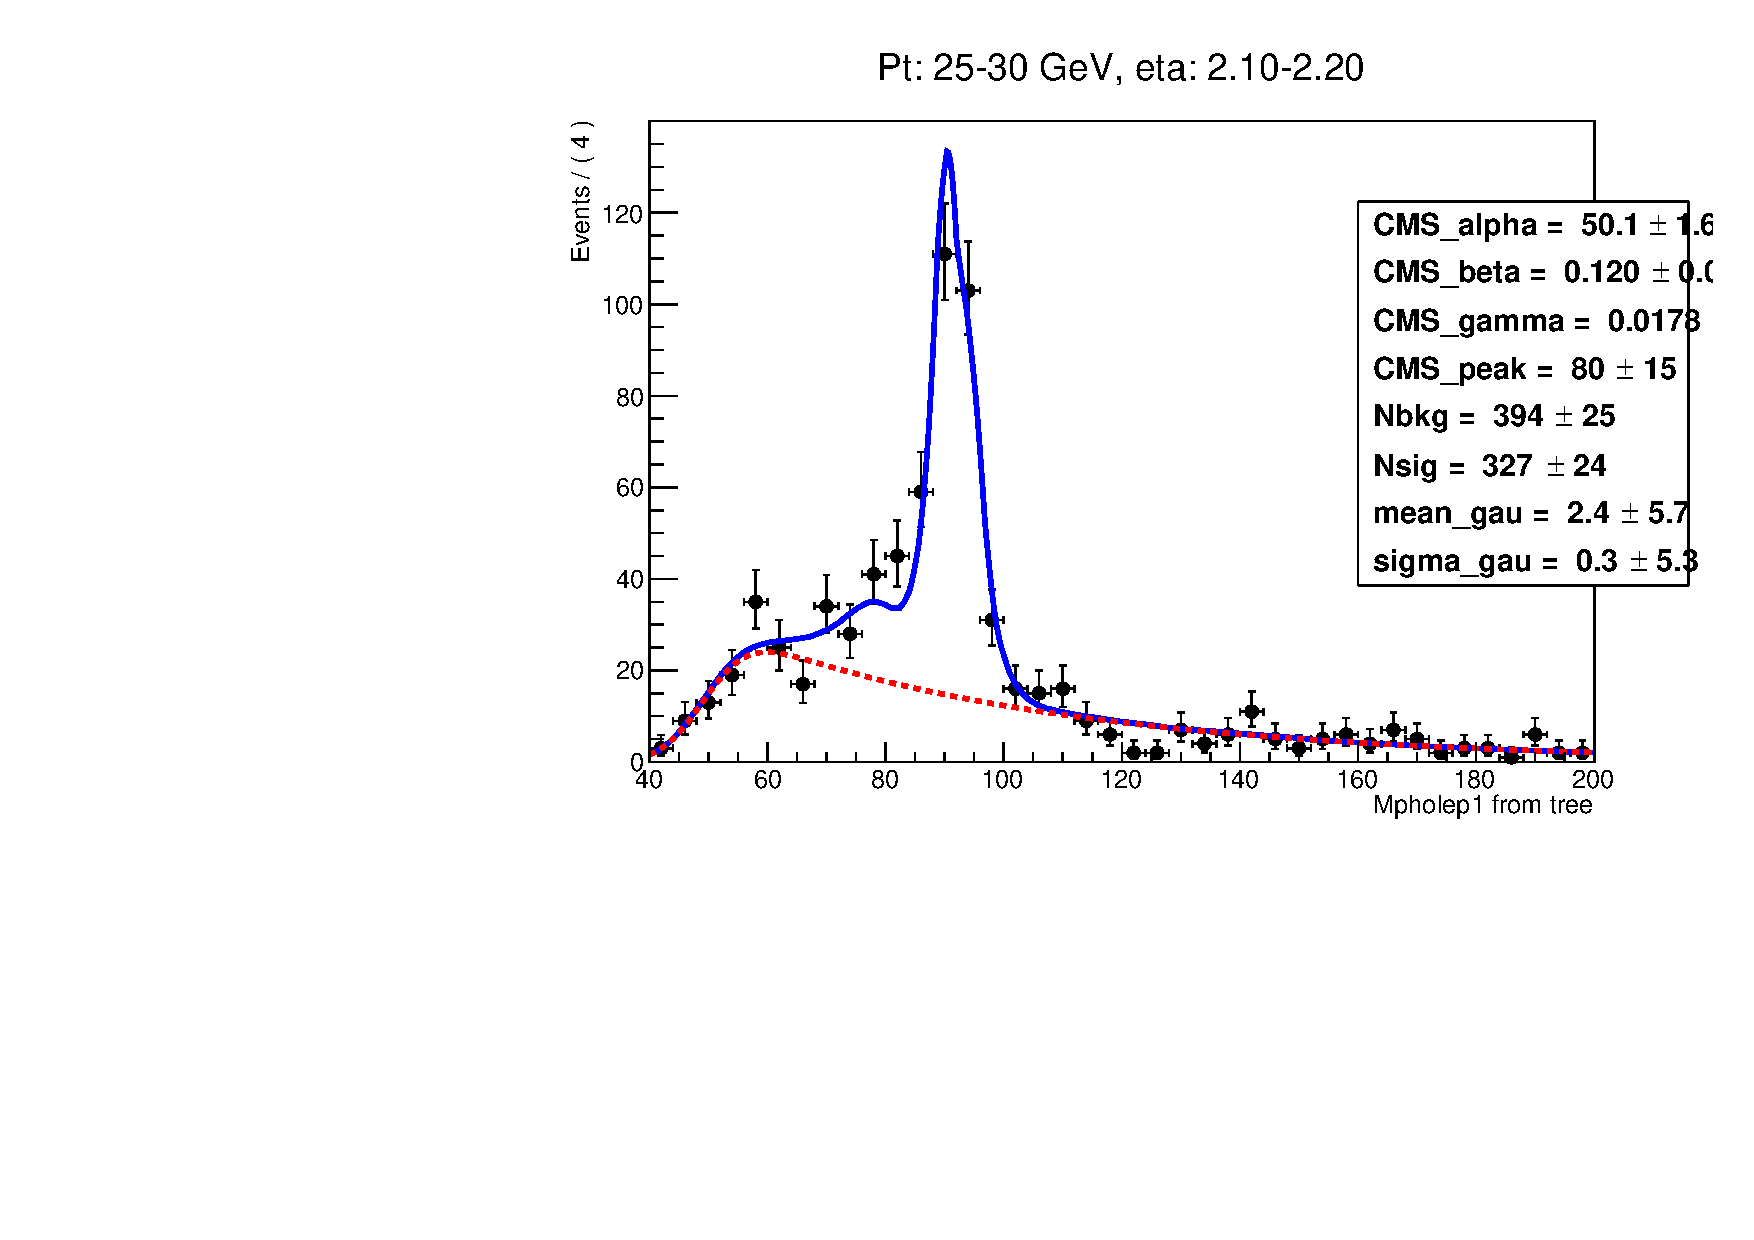
\includegraphics[width=0.45\textwidth]{../figs/figs_v11/ELECTRON_WGamma/EtoGammaFits/sa_hZmass_h_Data_EtoGamma_Enr_ENDCAP_pt25to30_ieta1.pdf}\\
   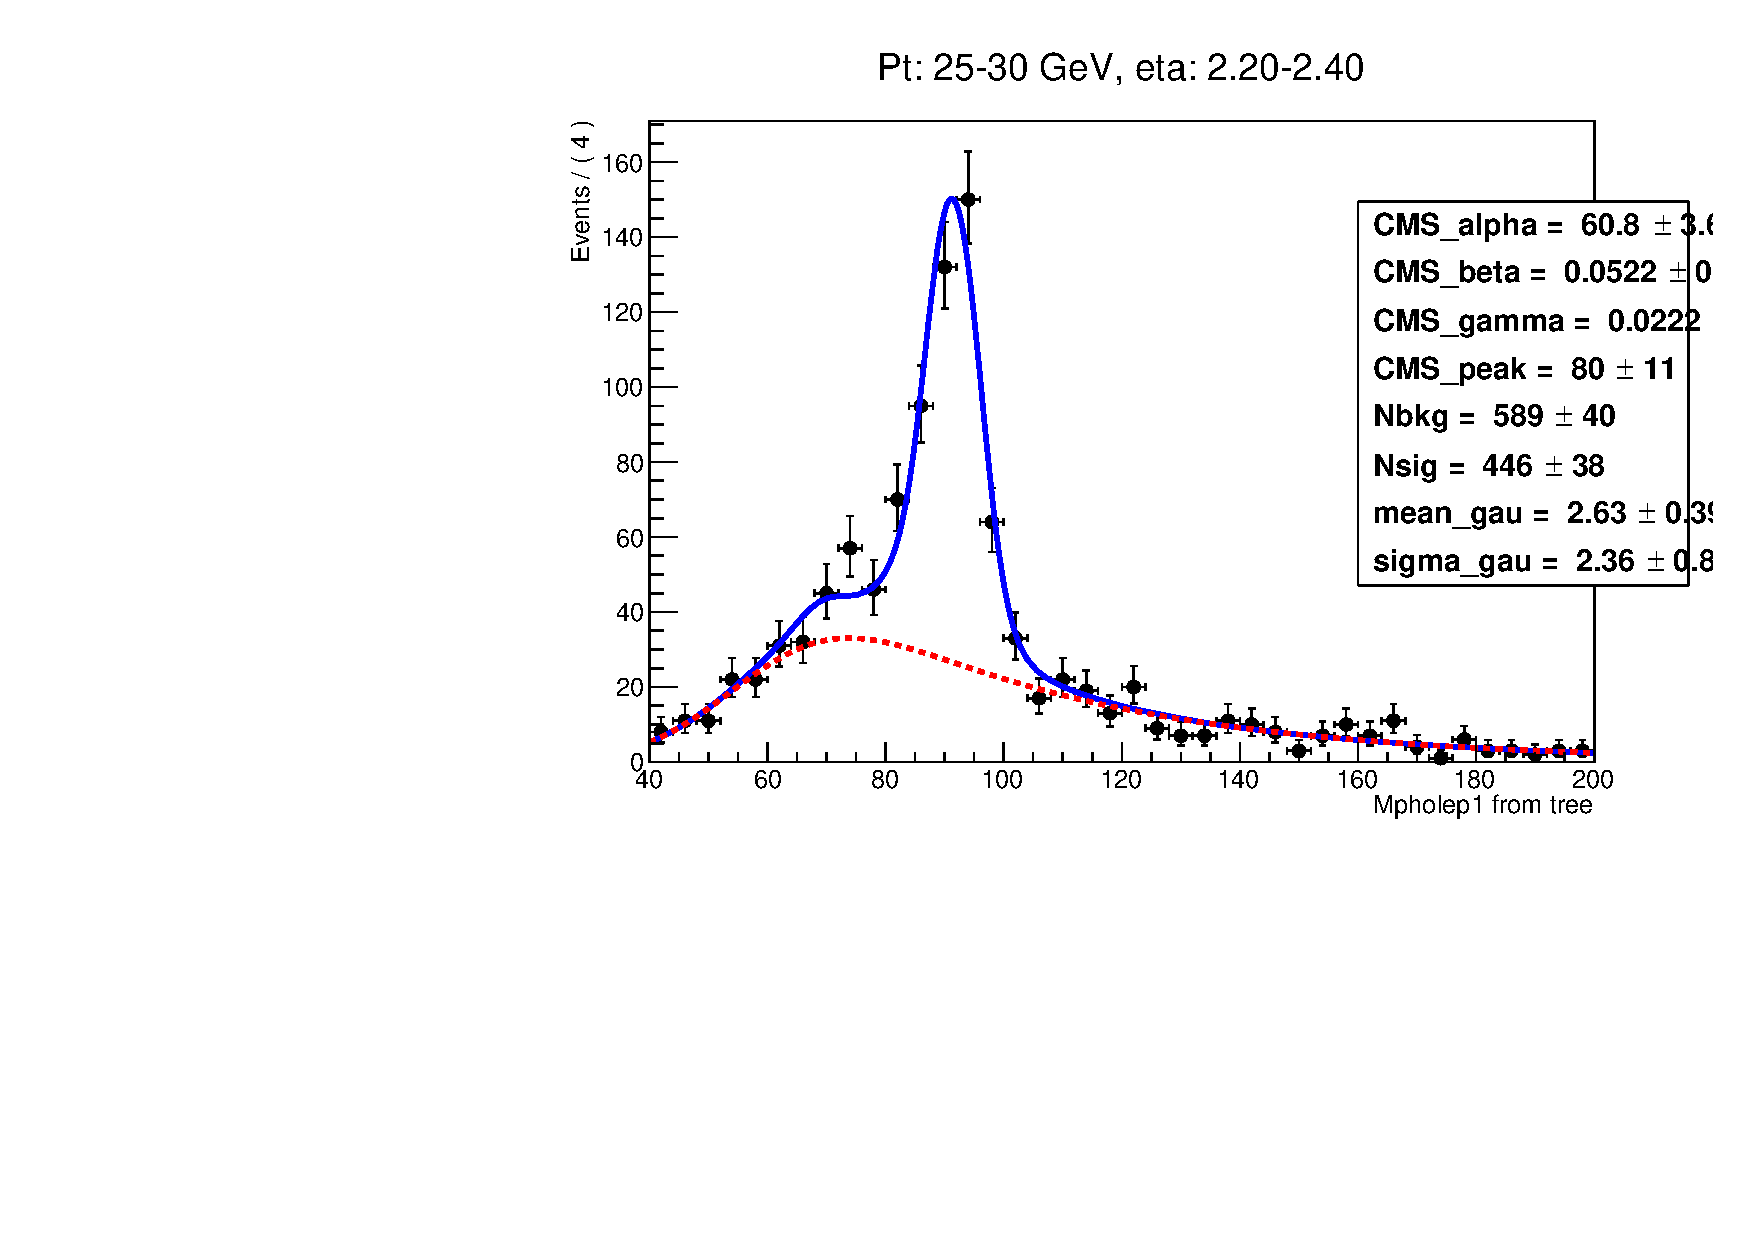
\includegraphics[width=0.45\textwidth]{../figs/figs_v11/ELECTRON_WGamma/EtoGammaFits/sa_hZmass_h_Data_EtoGamma_Enr_ENDCAP_pt25to30_ieta2.pdf}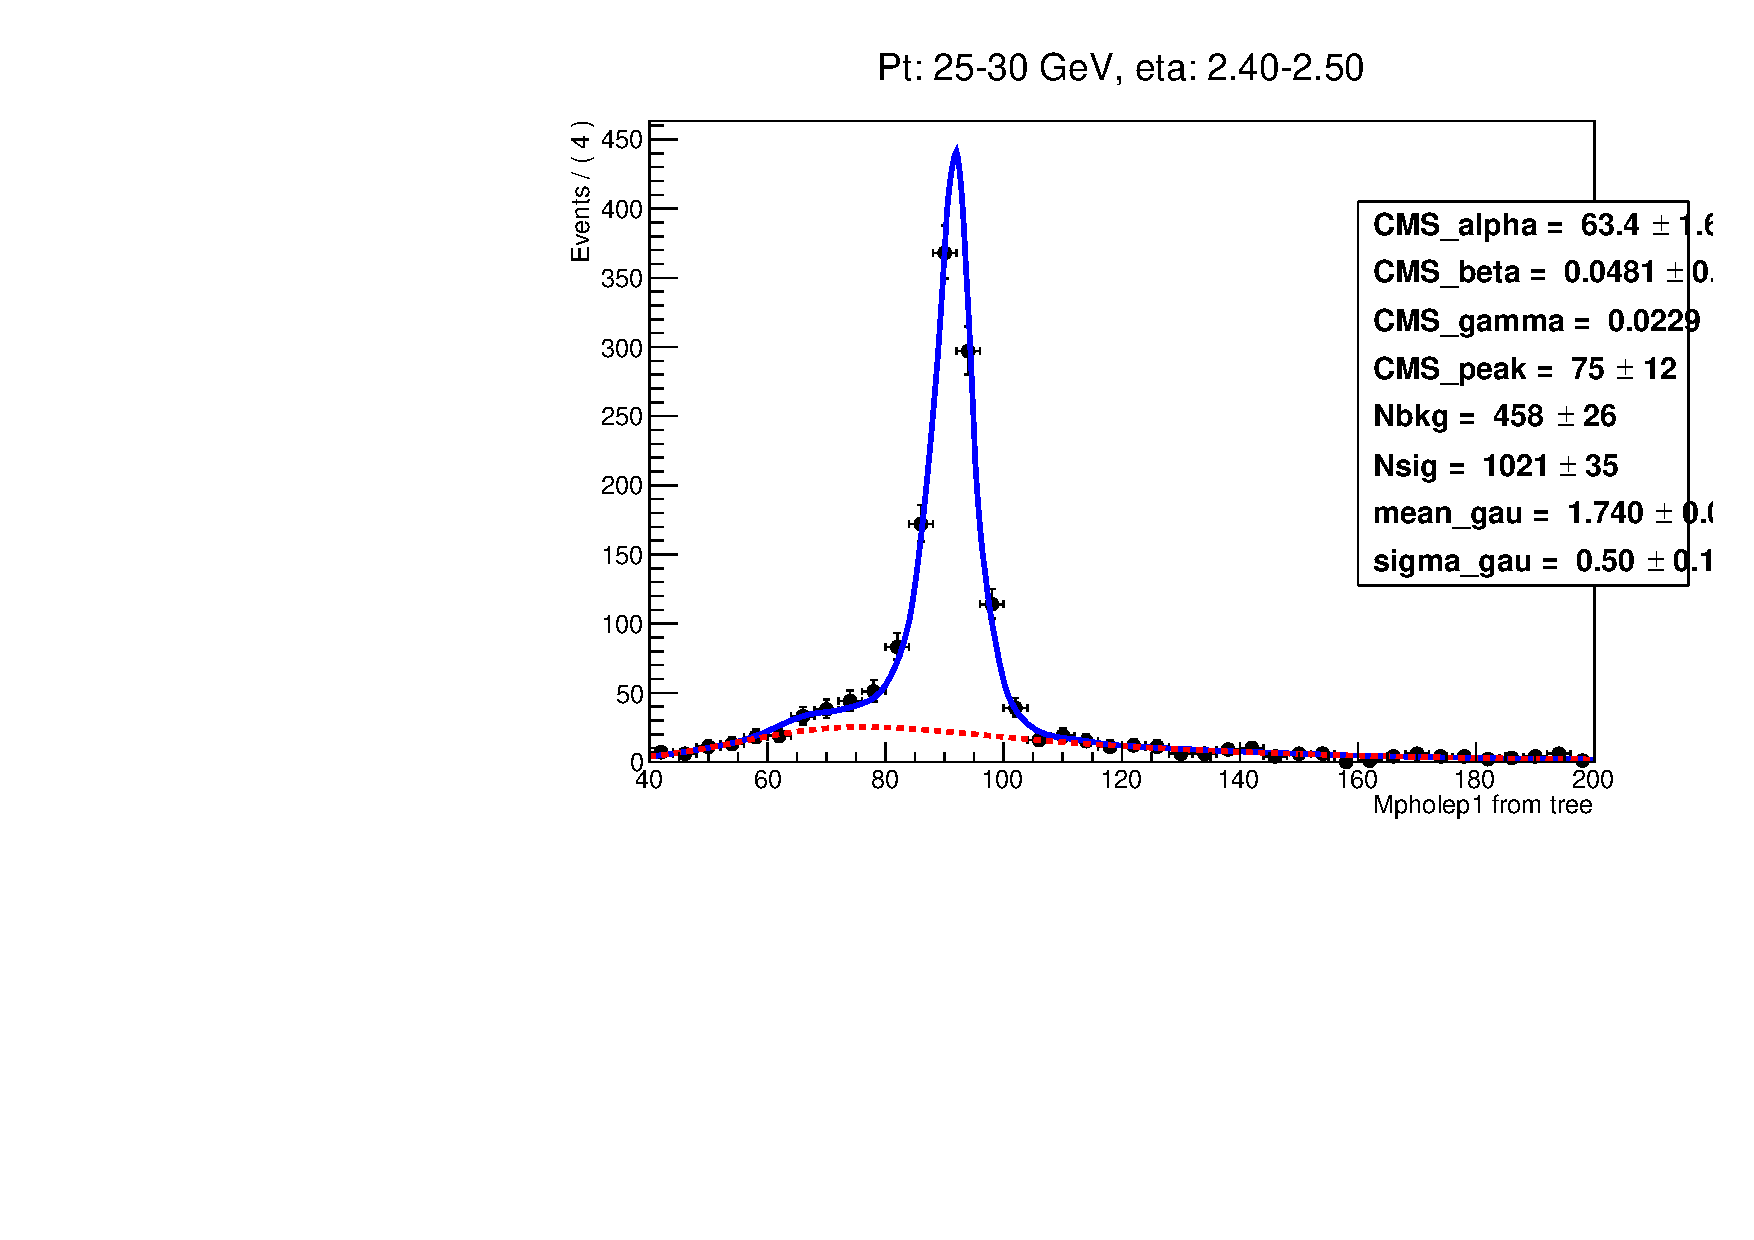
\includegraphics[width=0.45\textwidth]{../figs/figs_v11/ELECTRON_WGamma/EtoGammaFits/sa_hZmass_h_Data_EtoGamma_Enr_ENDCAP_pt25to30_ieta3.pdf}\\
  \label{fig:etogFits_25to30}
  \caption{$M_{e,\gamma}$ fits, W$\gamma$, electron channel, underflow bin (25-30 GeV), 8 eta bins}
  \end{center}
\end{figure}

\begin{figure}[htb]
  \begin{center}
   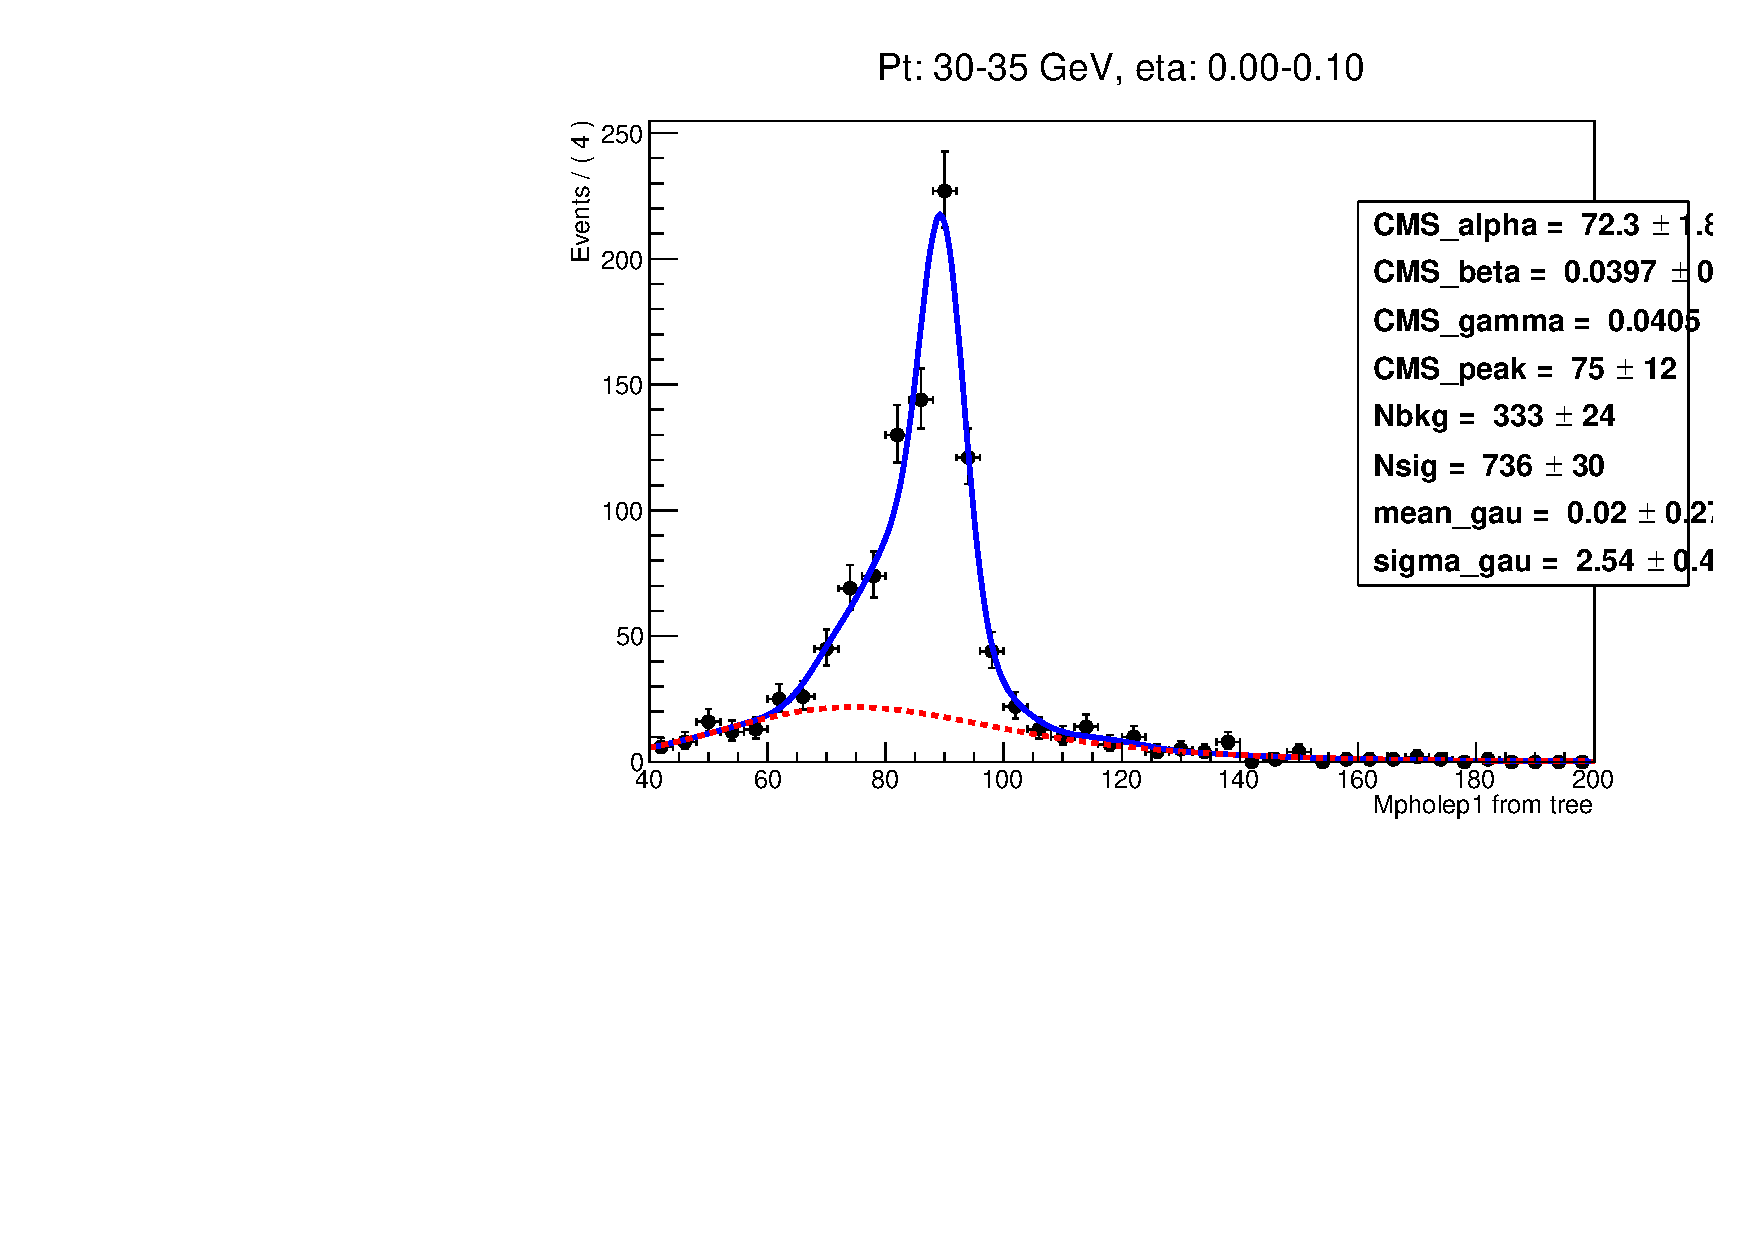
\includegraphics[width=0.45\textwidth]{../figs/figs_v11/ELECTRON_WGamma/EtoGammaFits/sa_hZmass_h_Data_EtoGamma_Enr_BARREL_pt30to35_ieta0.pdf}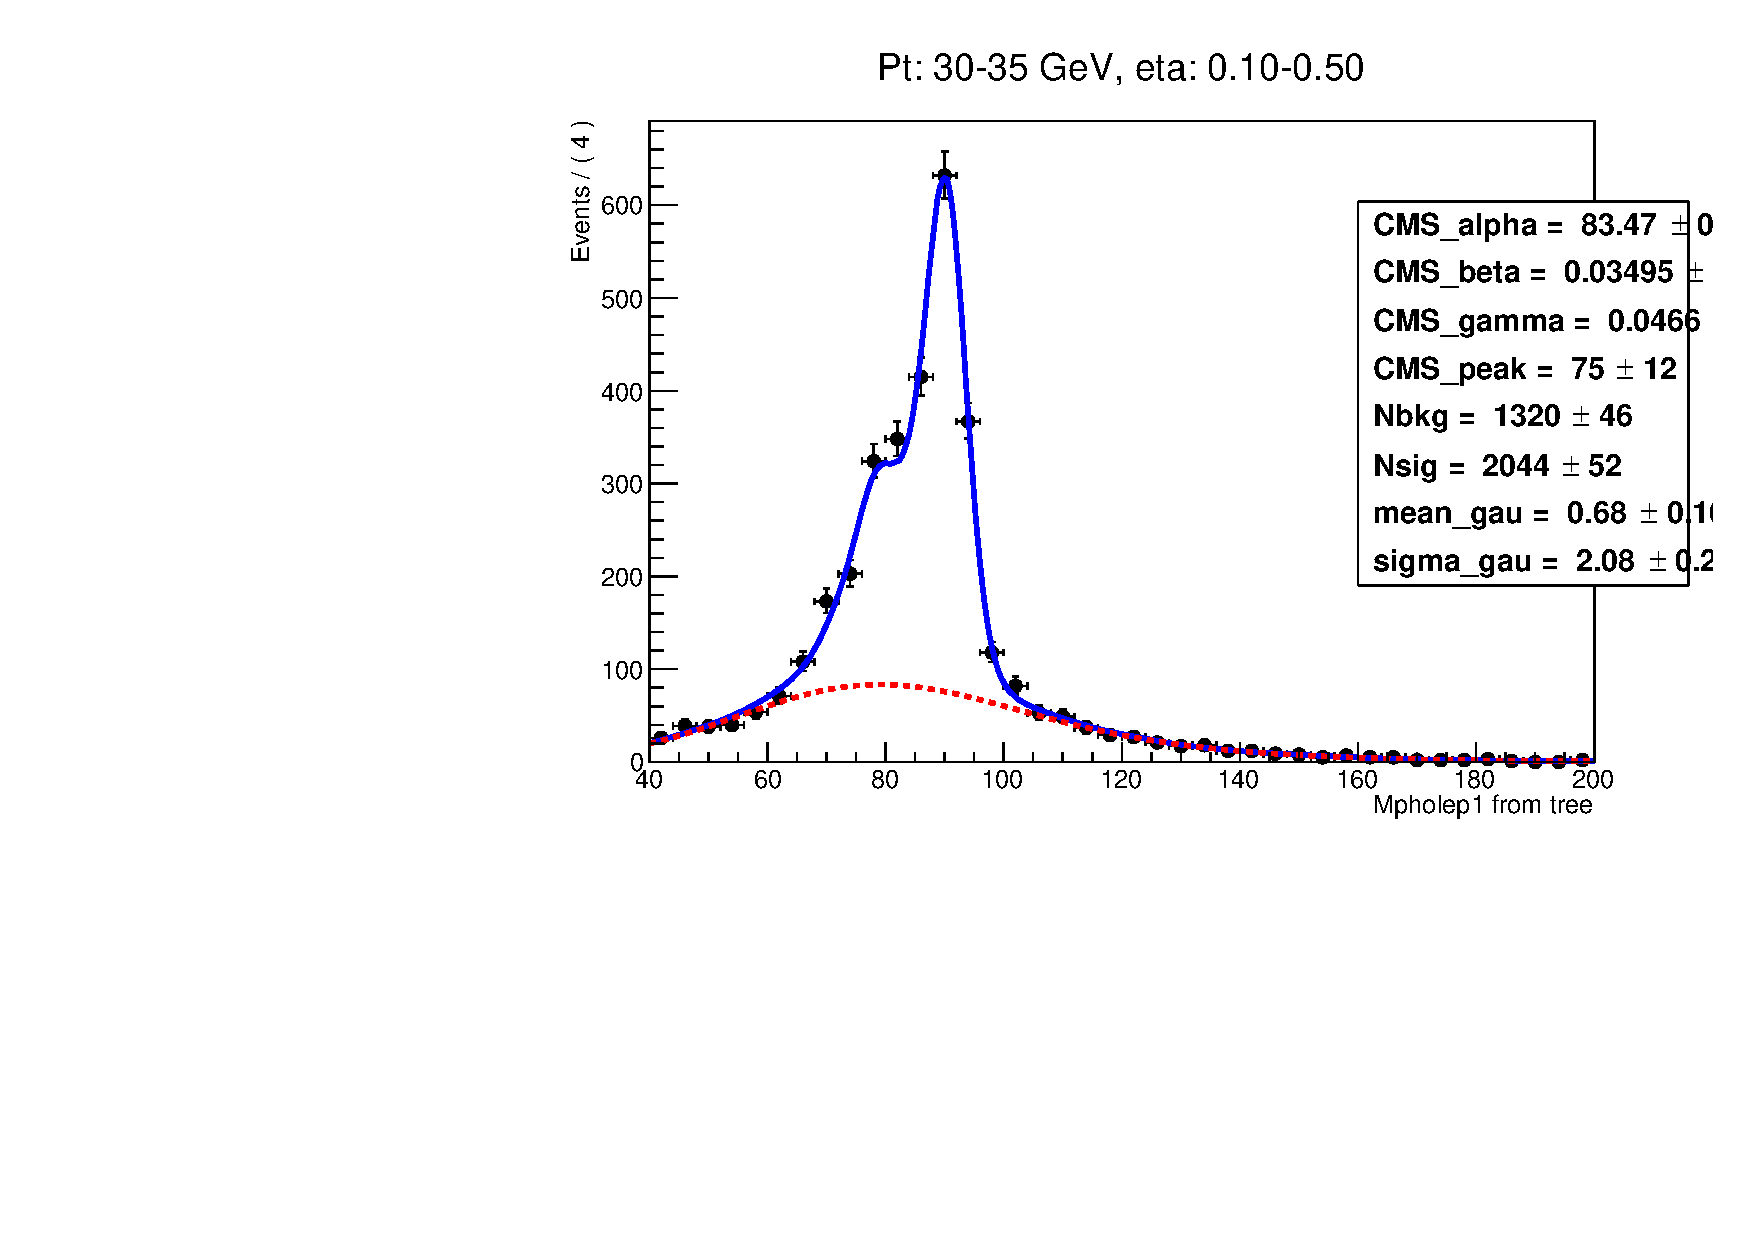
\includegraphics[width=0.45\textwidth]{../figs/figs_v11/ELECTRON_WGamma/EtoGammaFits/sa_hZmass_h_Data_EtoGamma_Enr_BARREL_pt30to35_ieta1.pdf}\\
   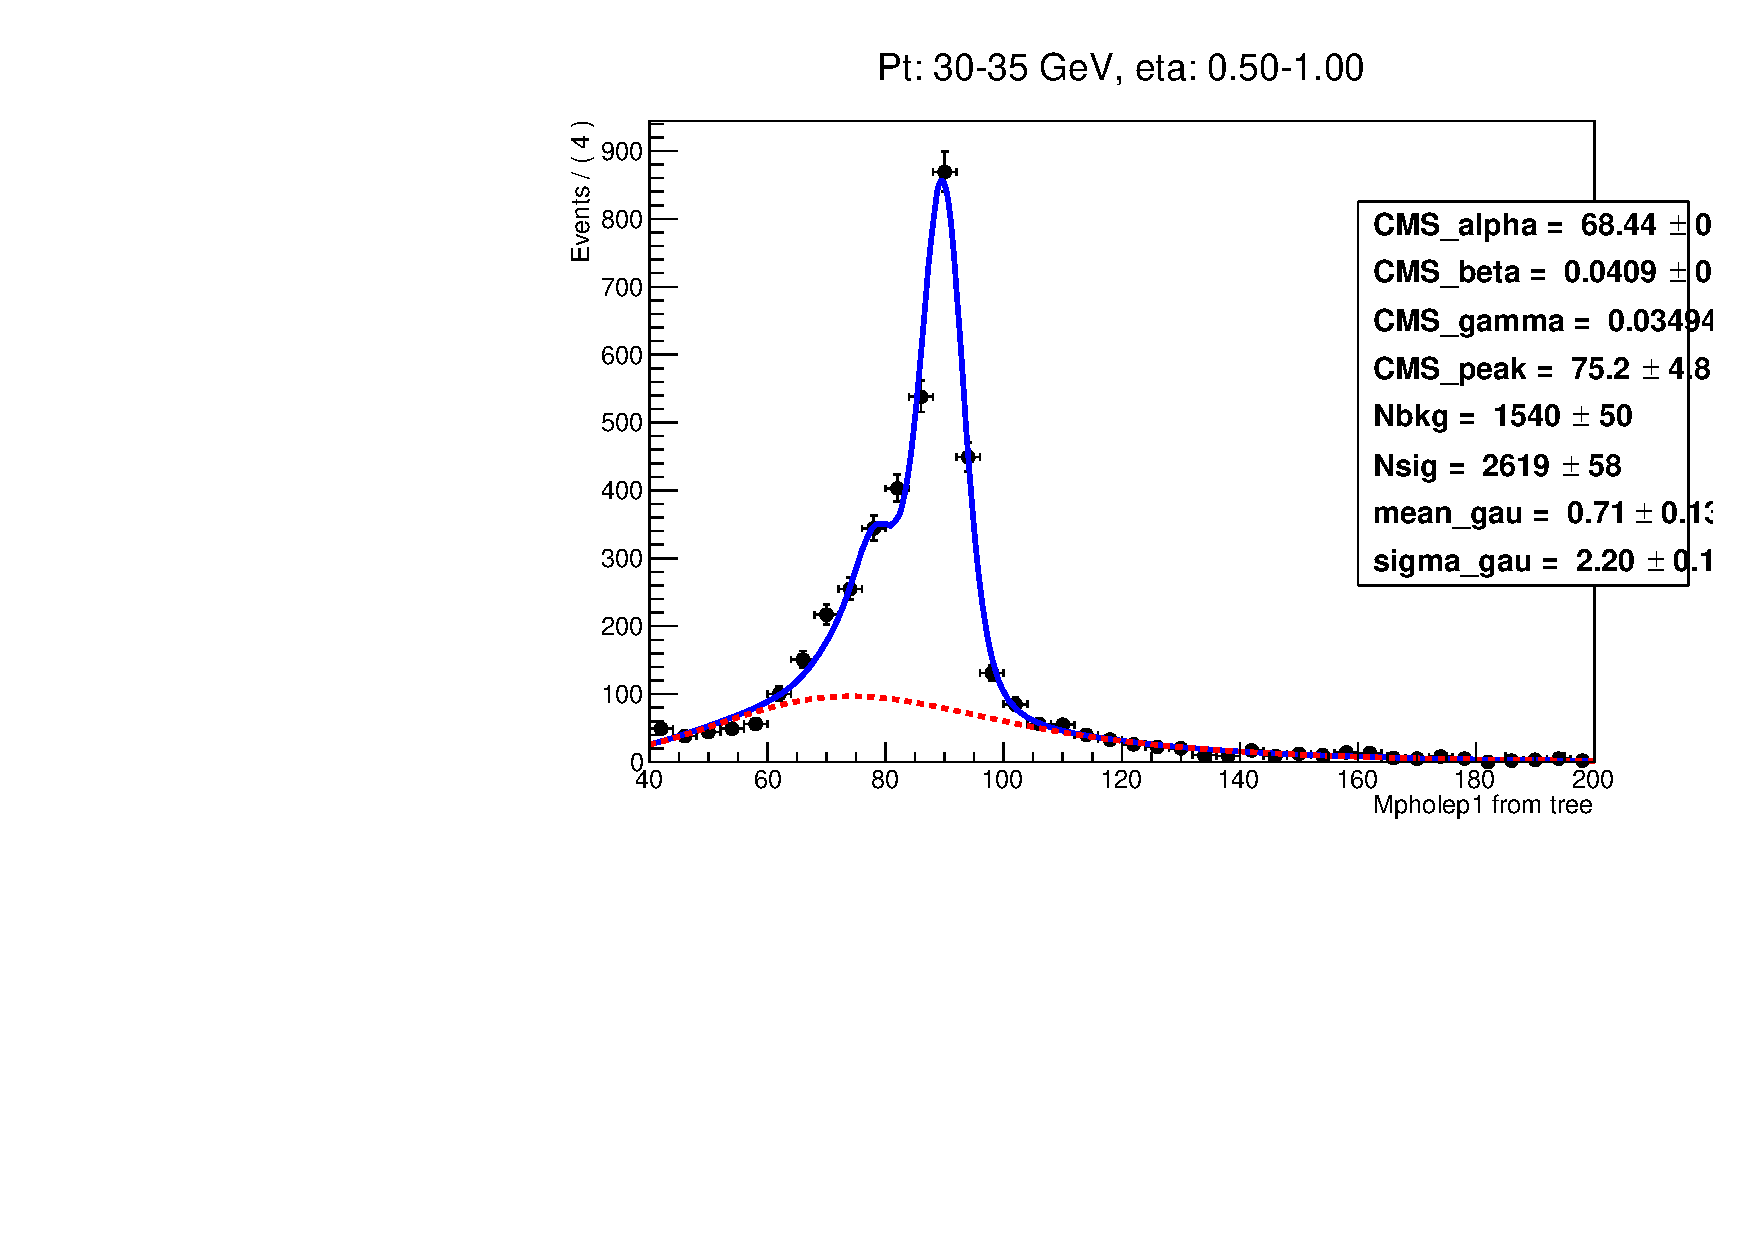
\includegraphics[width=0.45\textwidth]{../figs/figs_v11/ELECTRON_WGamma/EtoGammaFits/sa_hZmass_h_Data_EtoGamma_Enr_BARREL_pt30to35_ieta2.pdf}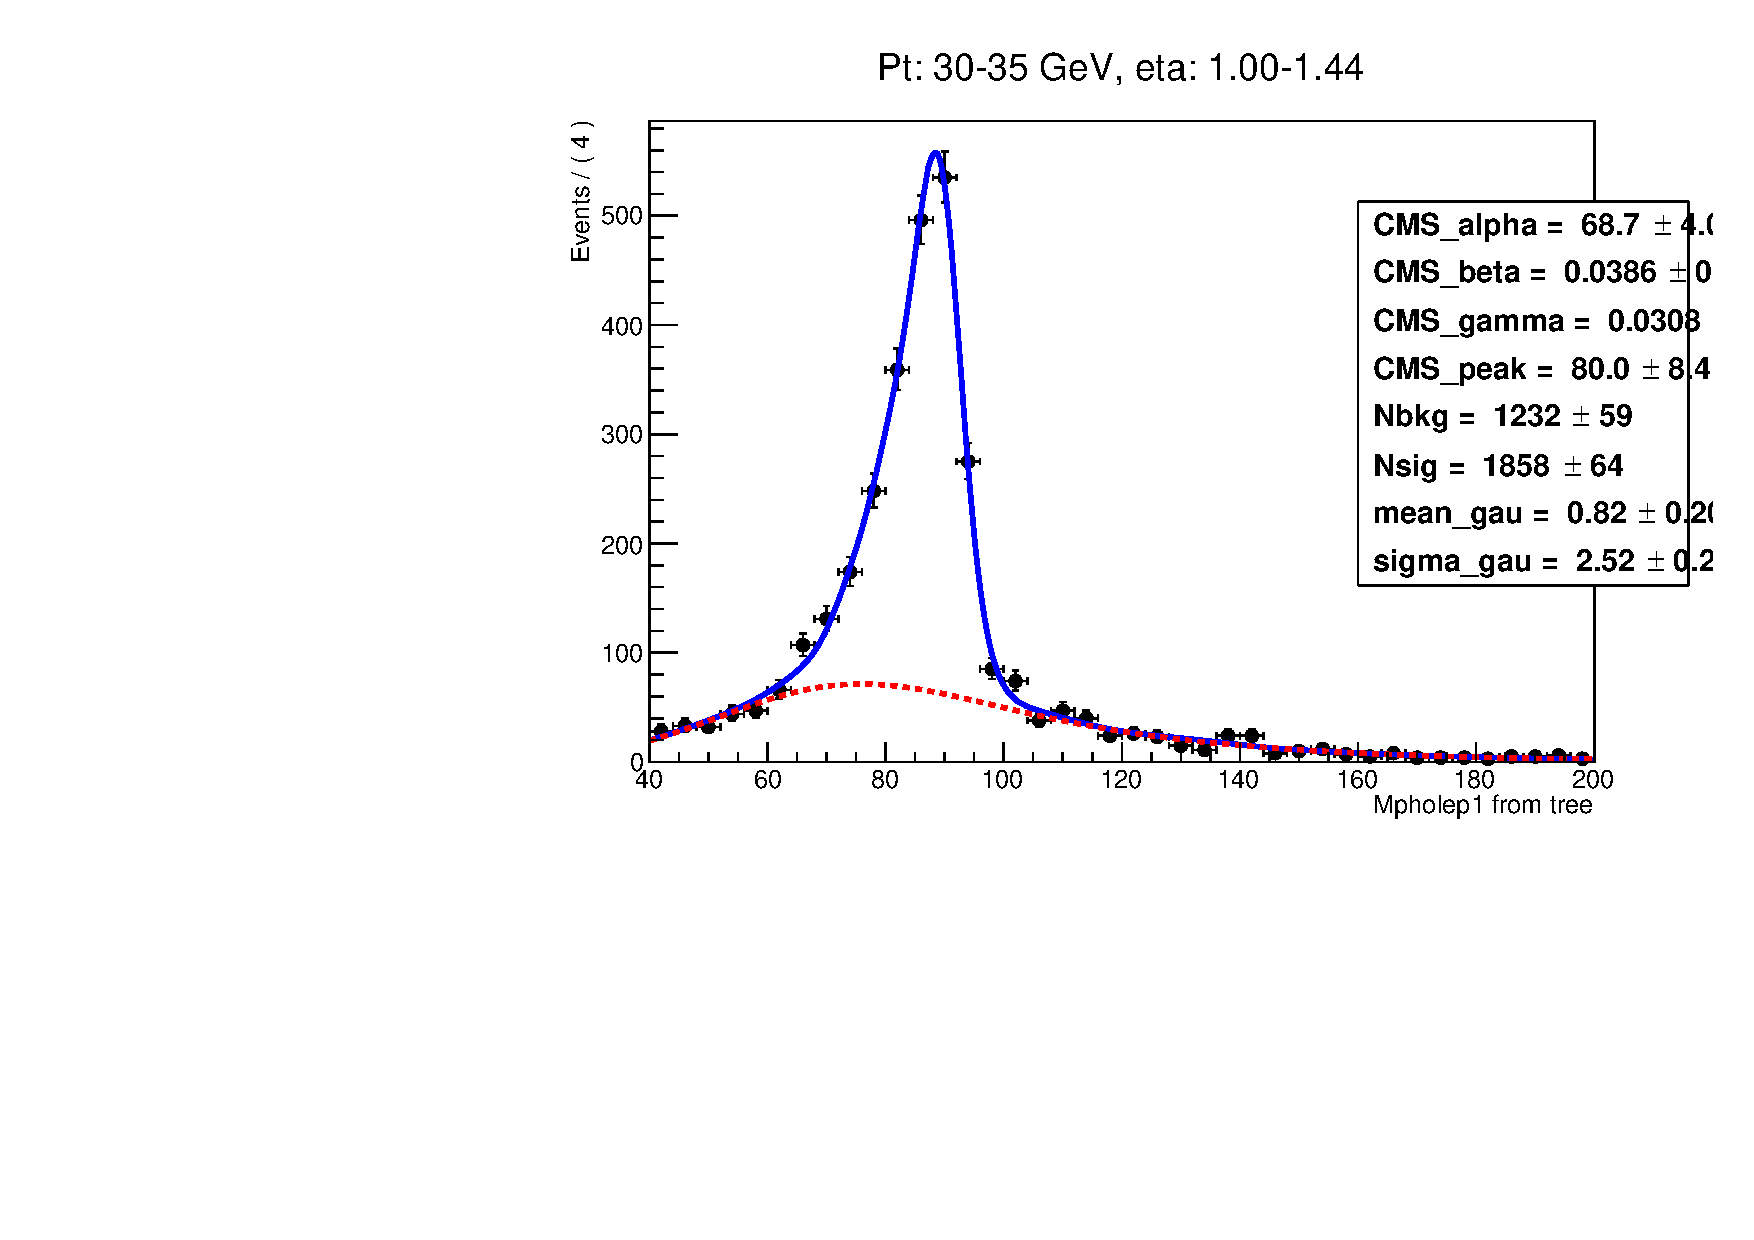
\includegraphics[width=0.45\textwidth]{../figs/figs_v11/ELECTRON_WGamma/EtoGammaFits/sa_hZmass_h_Data_EtoGamma_Enr_BARREL_pt30to35_ieta3.pdf}\\
   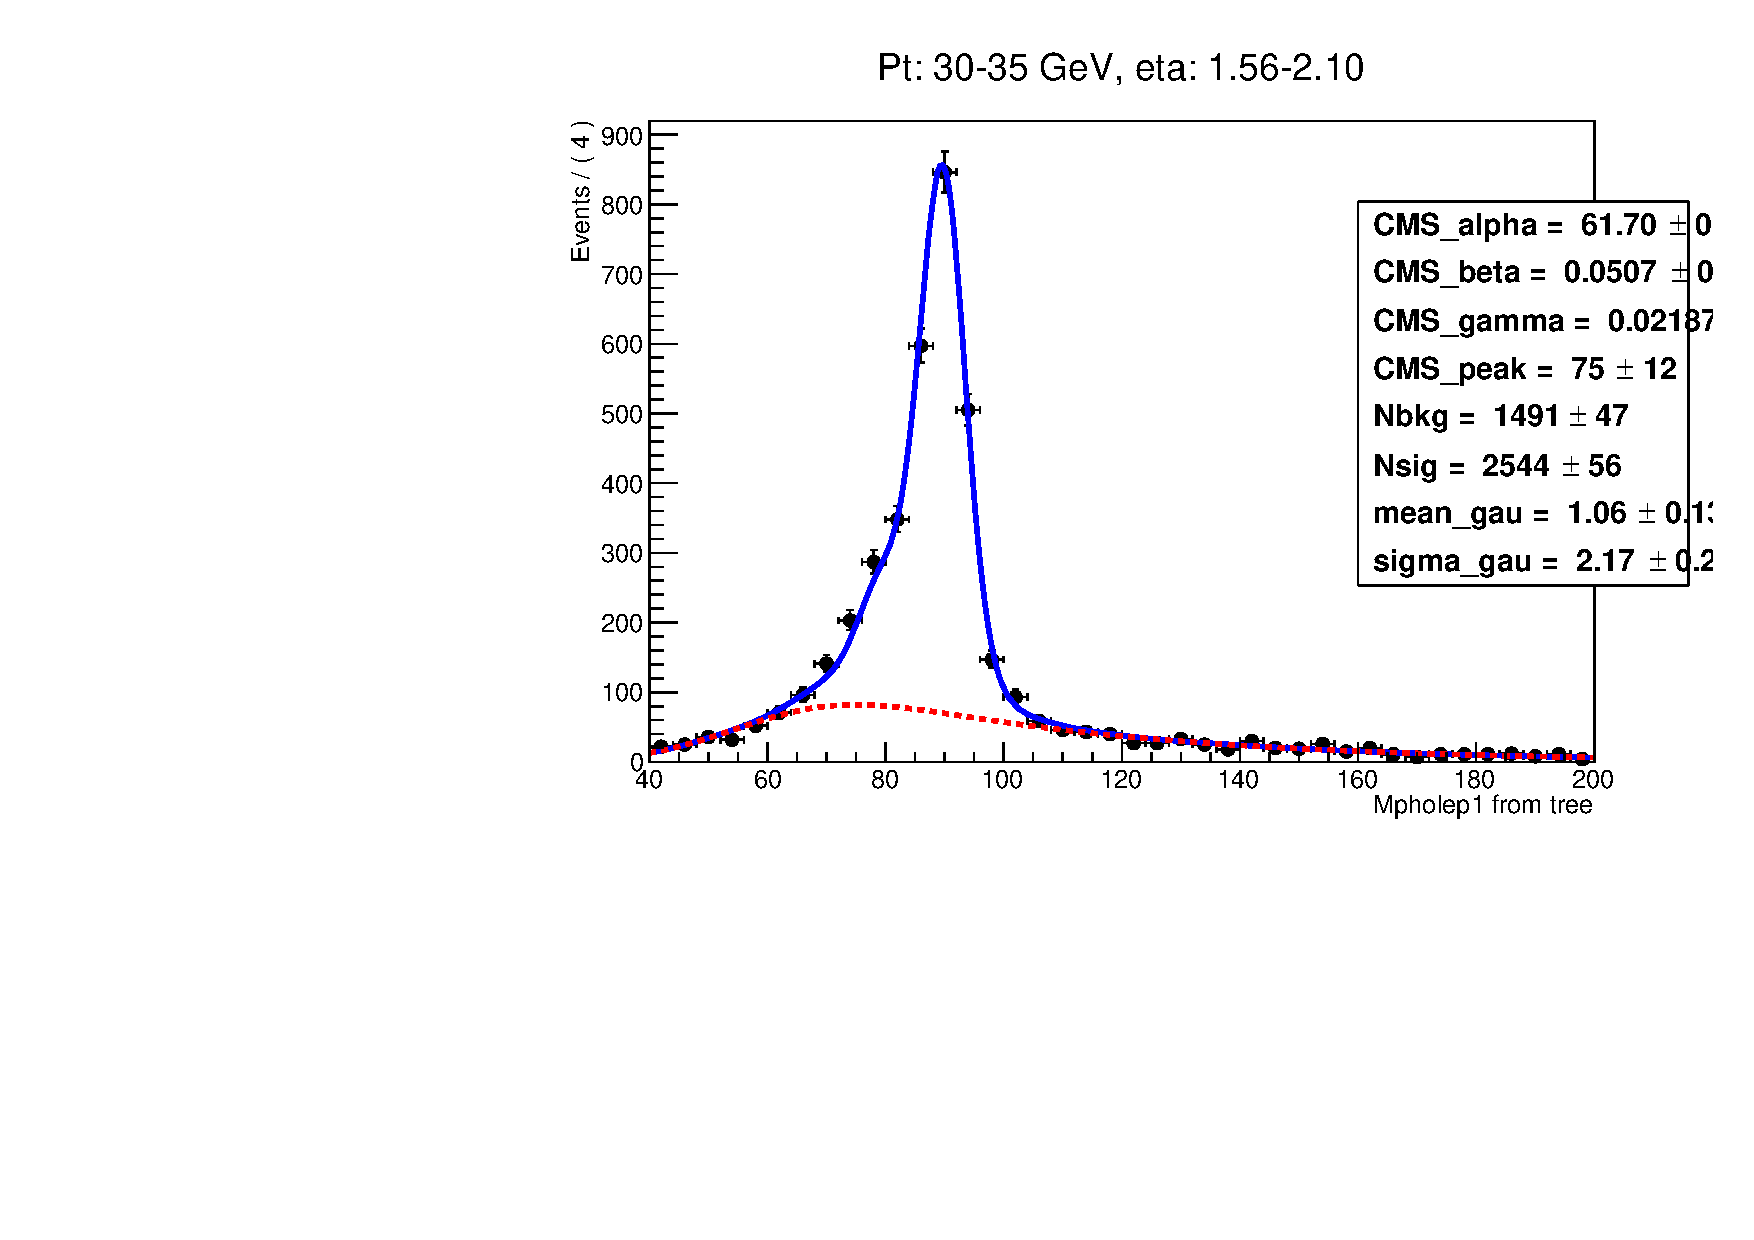
\includegraphics[width=0.45\textwidth]{../figs/figs_v11/ELECTRON_WGamma/EtoGammaFits/sa_hZmass_h_Data_EtoGamma_Enr_ENDCAP_pt30to35_ieta0.pdf}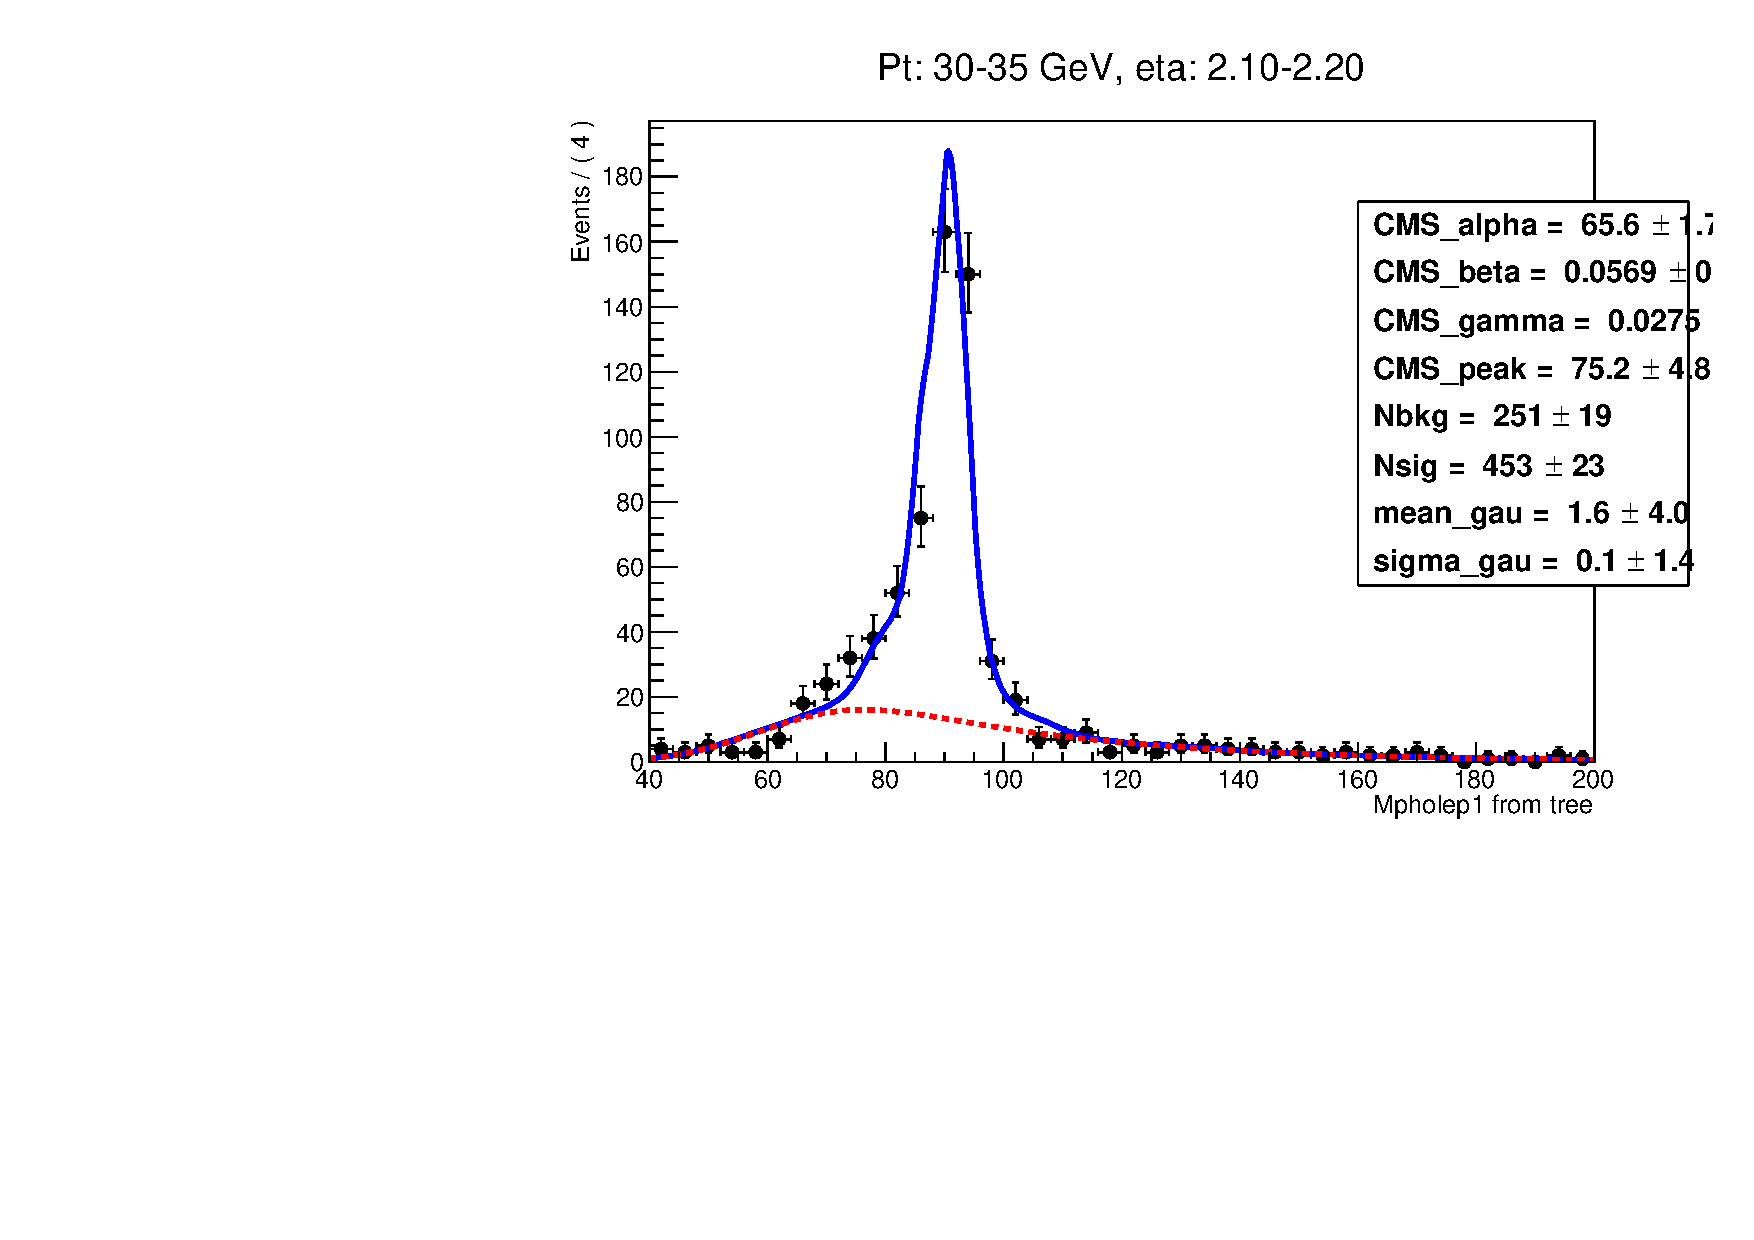
\includegraphics[width=0.45\textwidth]{../figs/figs_v11/ELECTRON_WGamma/EtoGammaFits/sa_hZmass_h_Data_EtoGamma_Enr_ENDCAP_pt30to35_ieta1.pdf}\\
   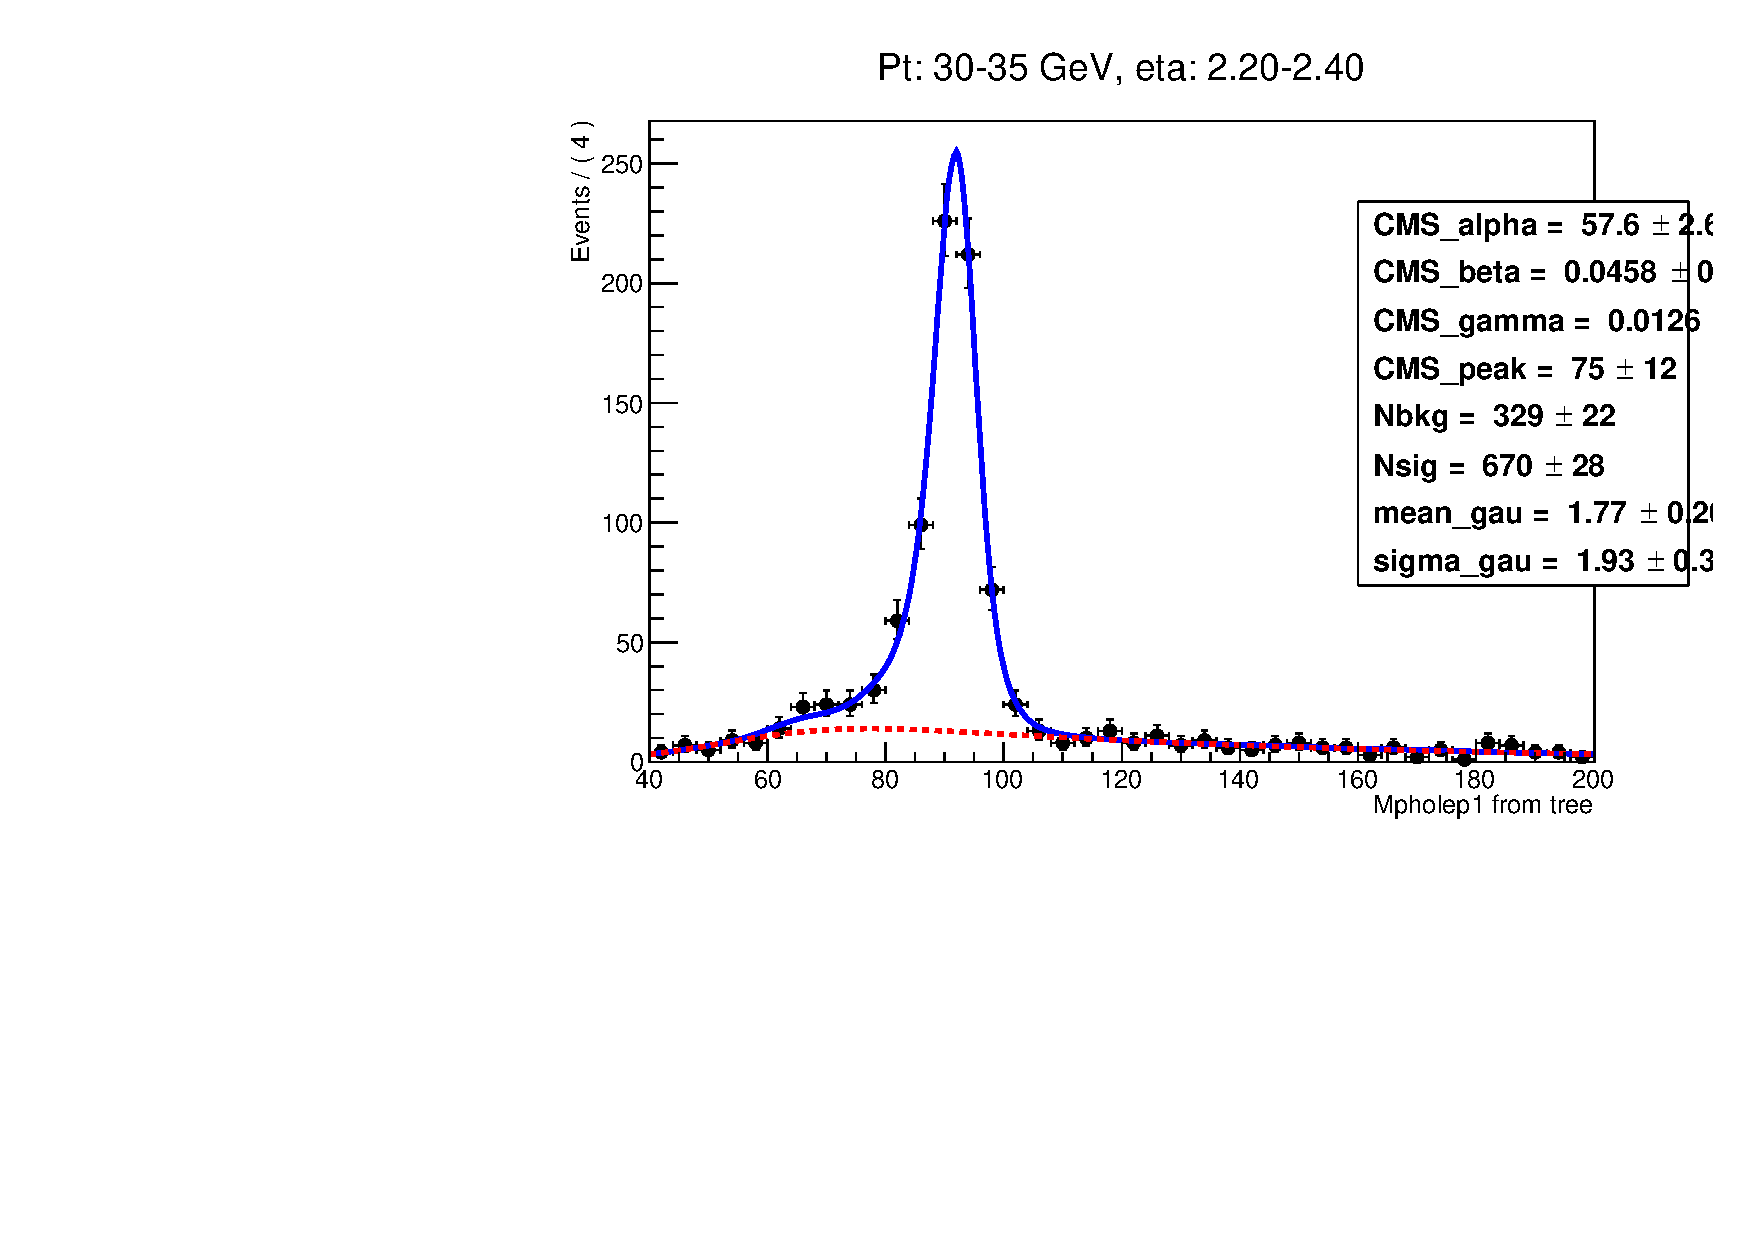
\includegraphics[width=0.45\textwidth]{../figs/figs_v11/ELECTRON_WGamma/EtoGammaFits/sa_hZmass_h_Data_EtoGamma_Enr_ENDCAP_pt30to35_ieta2.pdf}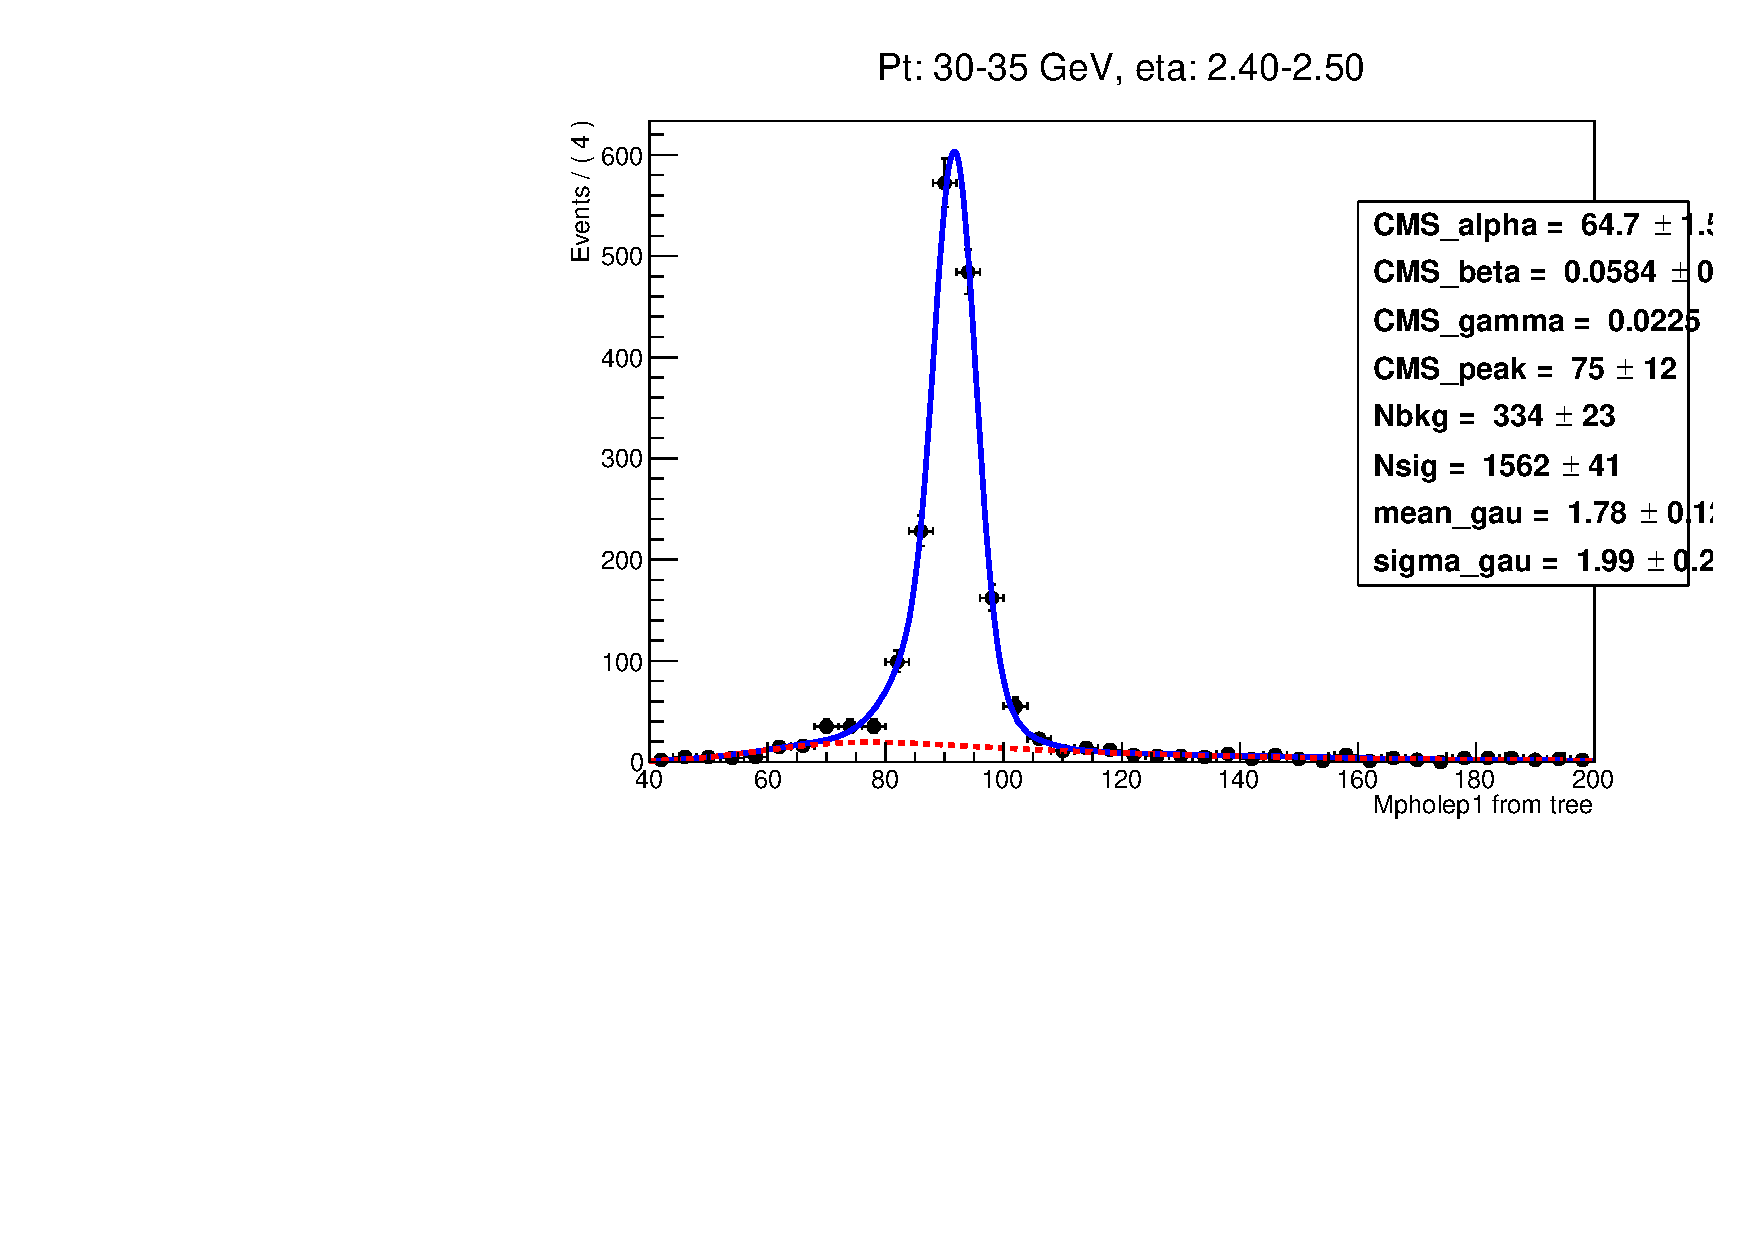
\includegraphics[width=0.45\textwidth]{../figs/figs_v11/ELECTRON_WGamma/EtoGammaFits/sa_hZmass_h_Data_EtoGamma_Enr_ENDCAP_pt30to35_ieta3.pdf}\\
  \label{fig:etogFits_30to35}
  \caption{$M_{e,\gamma}$ fits, W$\gamma$, electron channel, underflow bin (30-35 GeV), 8 eta bins}
  \end{center}
\end{figure}

\begin{figure}[htb]
  \begin{center}
   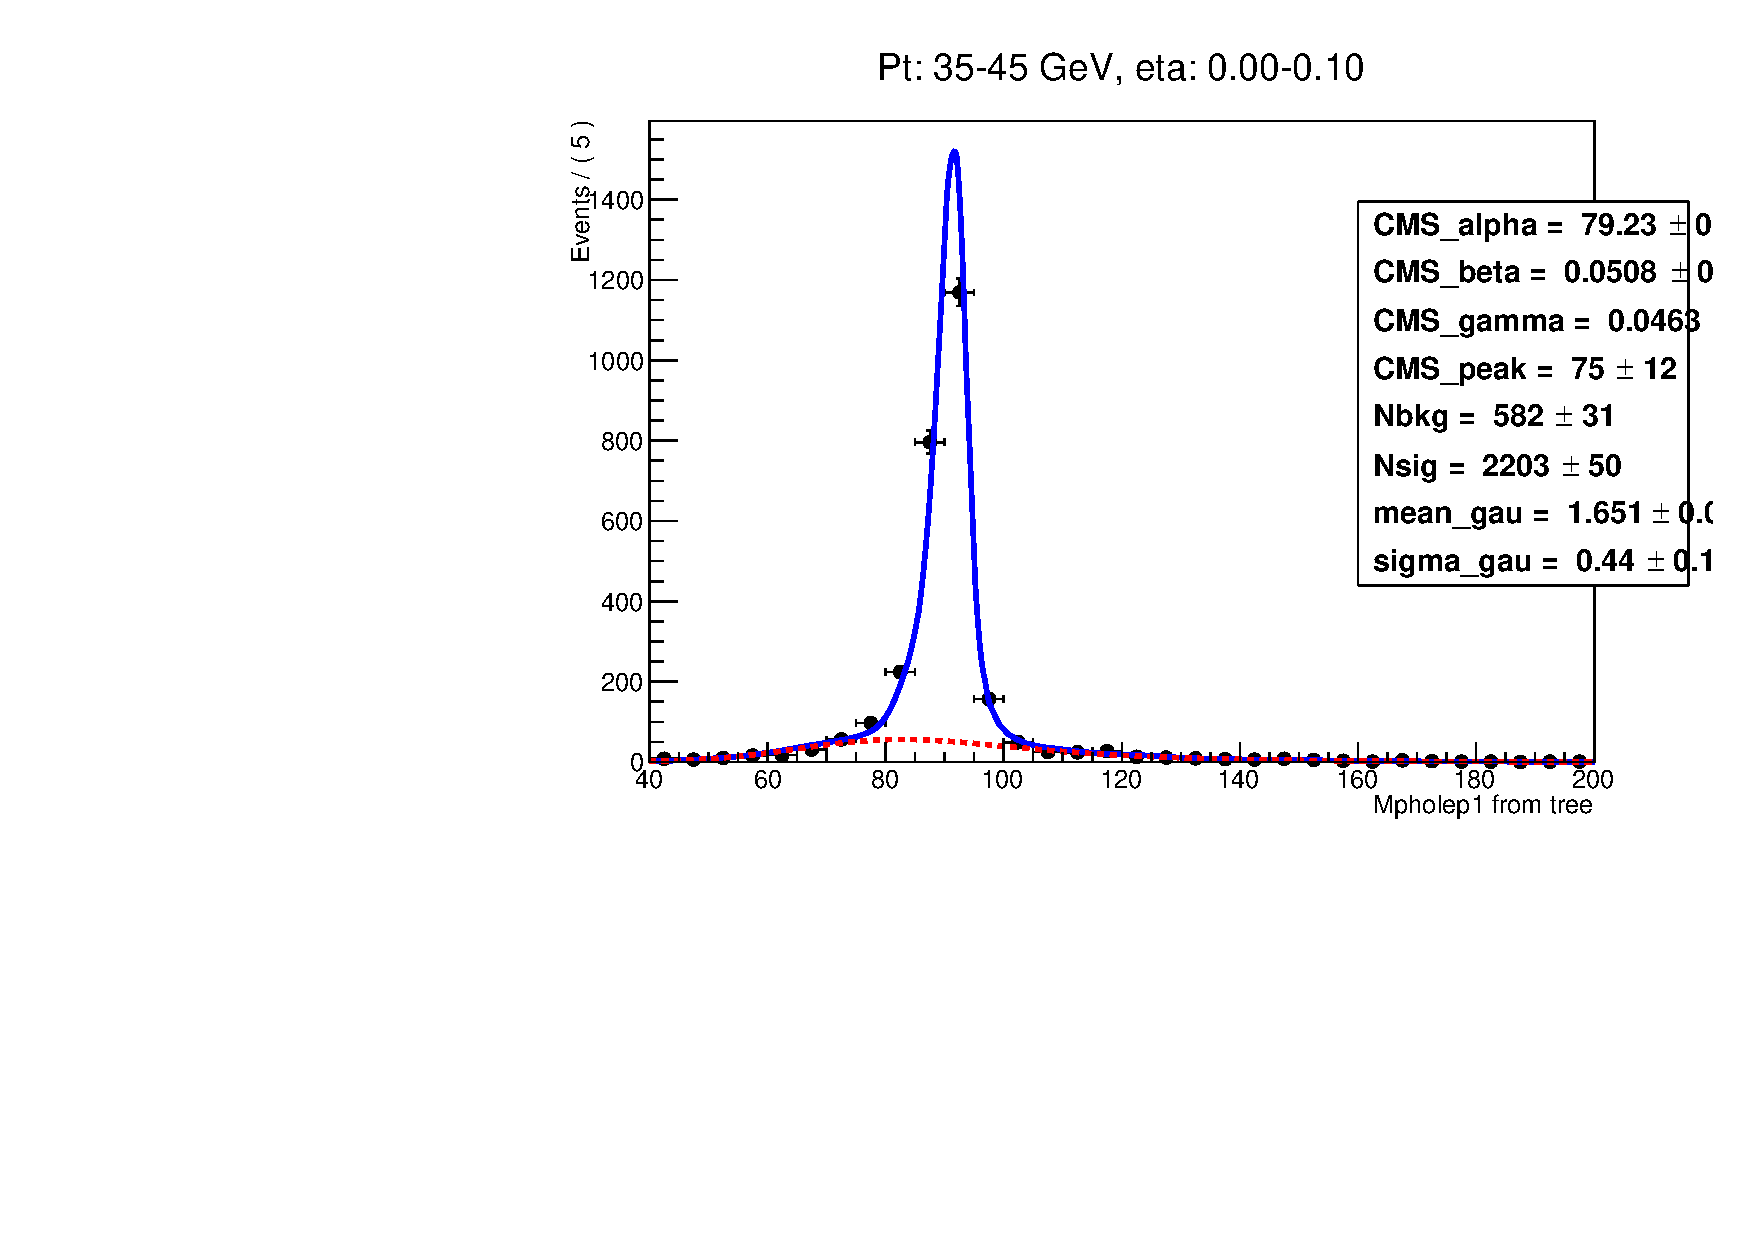
\includegraphics[width=0.45\textwidth]{../figs/figs_v11/ELECTRON_WGamma/EtoGammaFits/sa_hZmass_h_Data_EtoGamma_Enr_BARREL_pt35to45_ieta0.pdf}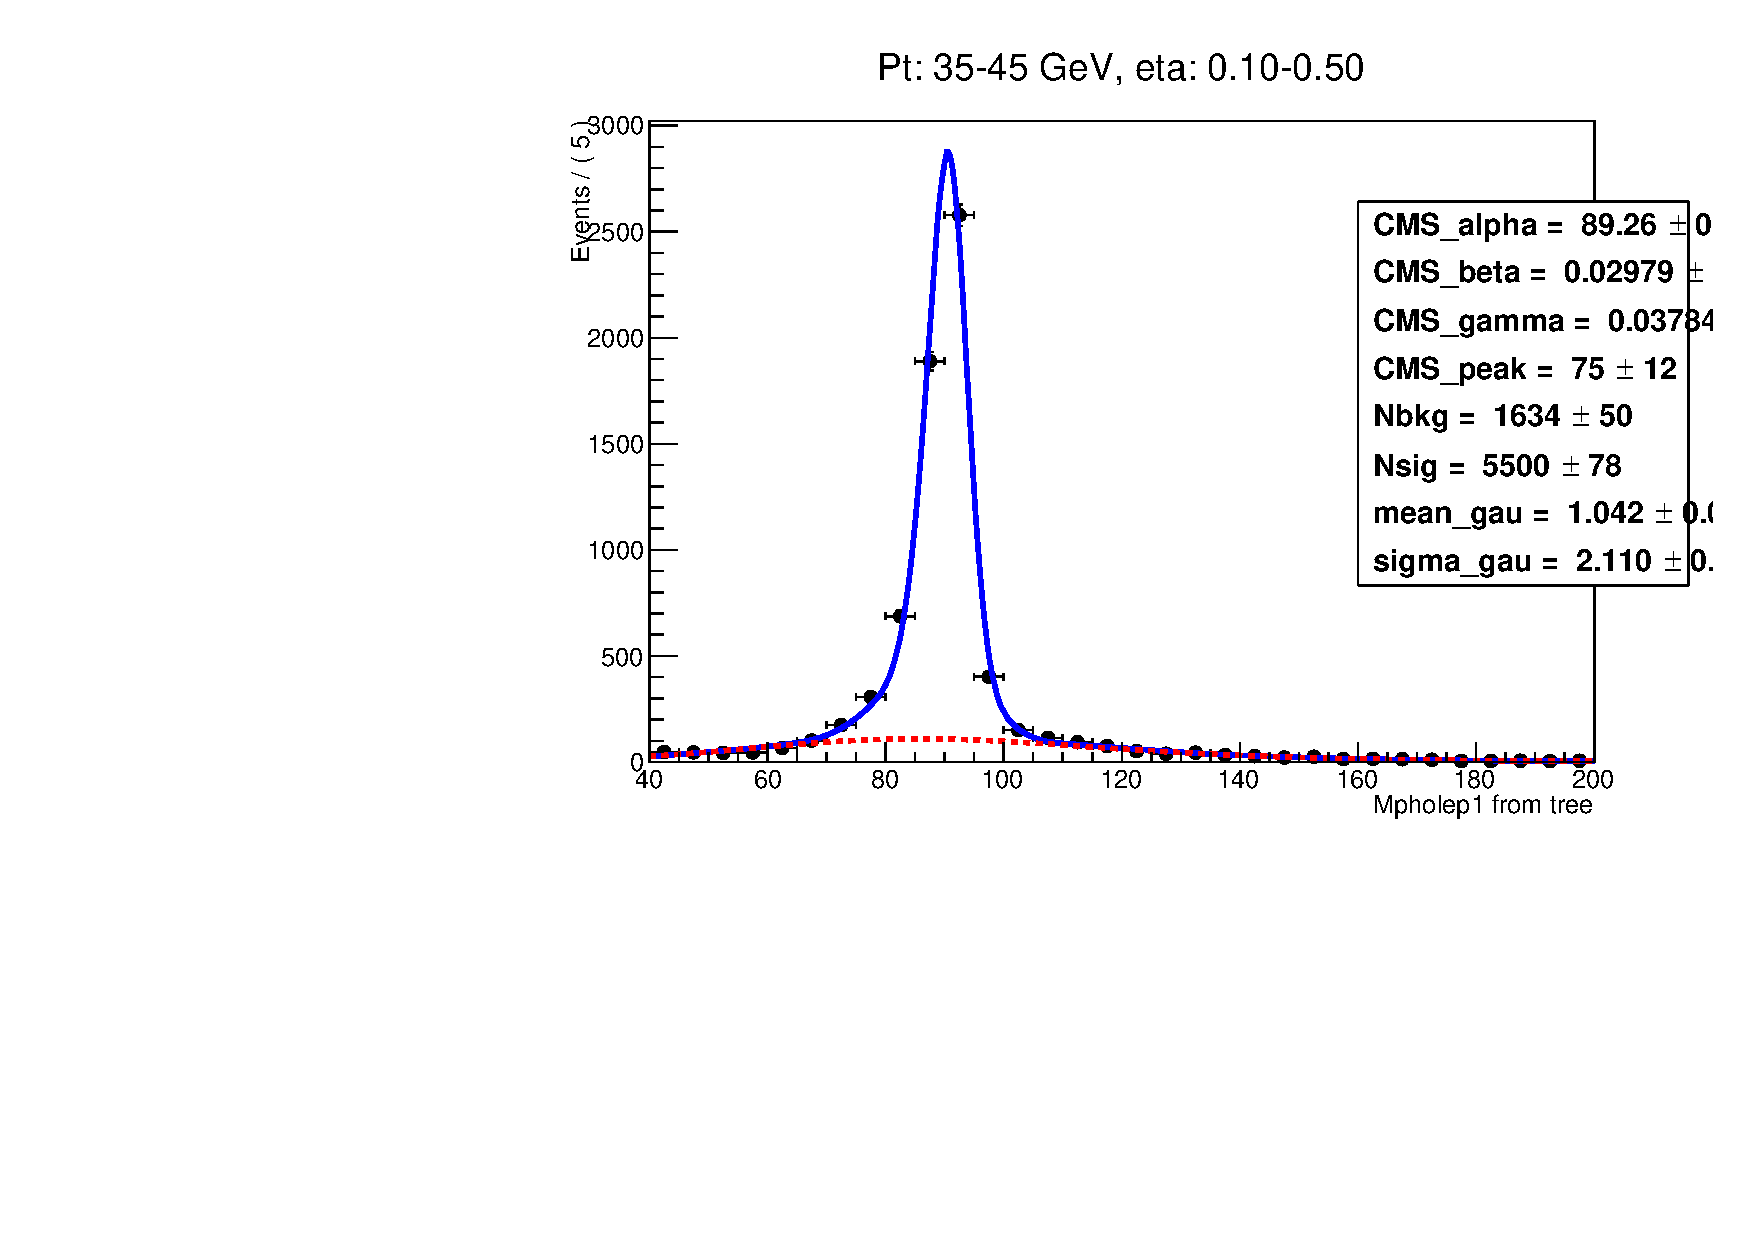
\includegraphics[width=0.45\textwidth]{../figs/figs_v11/ELECTRON_WGamma/EtoGammaFits/sa_hZmass_h_Data_EtoGamma_Enr_BARREL_pt35to45_ieta1.pdf}\\
   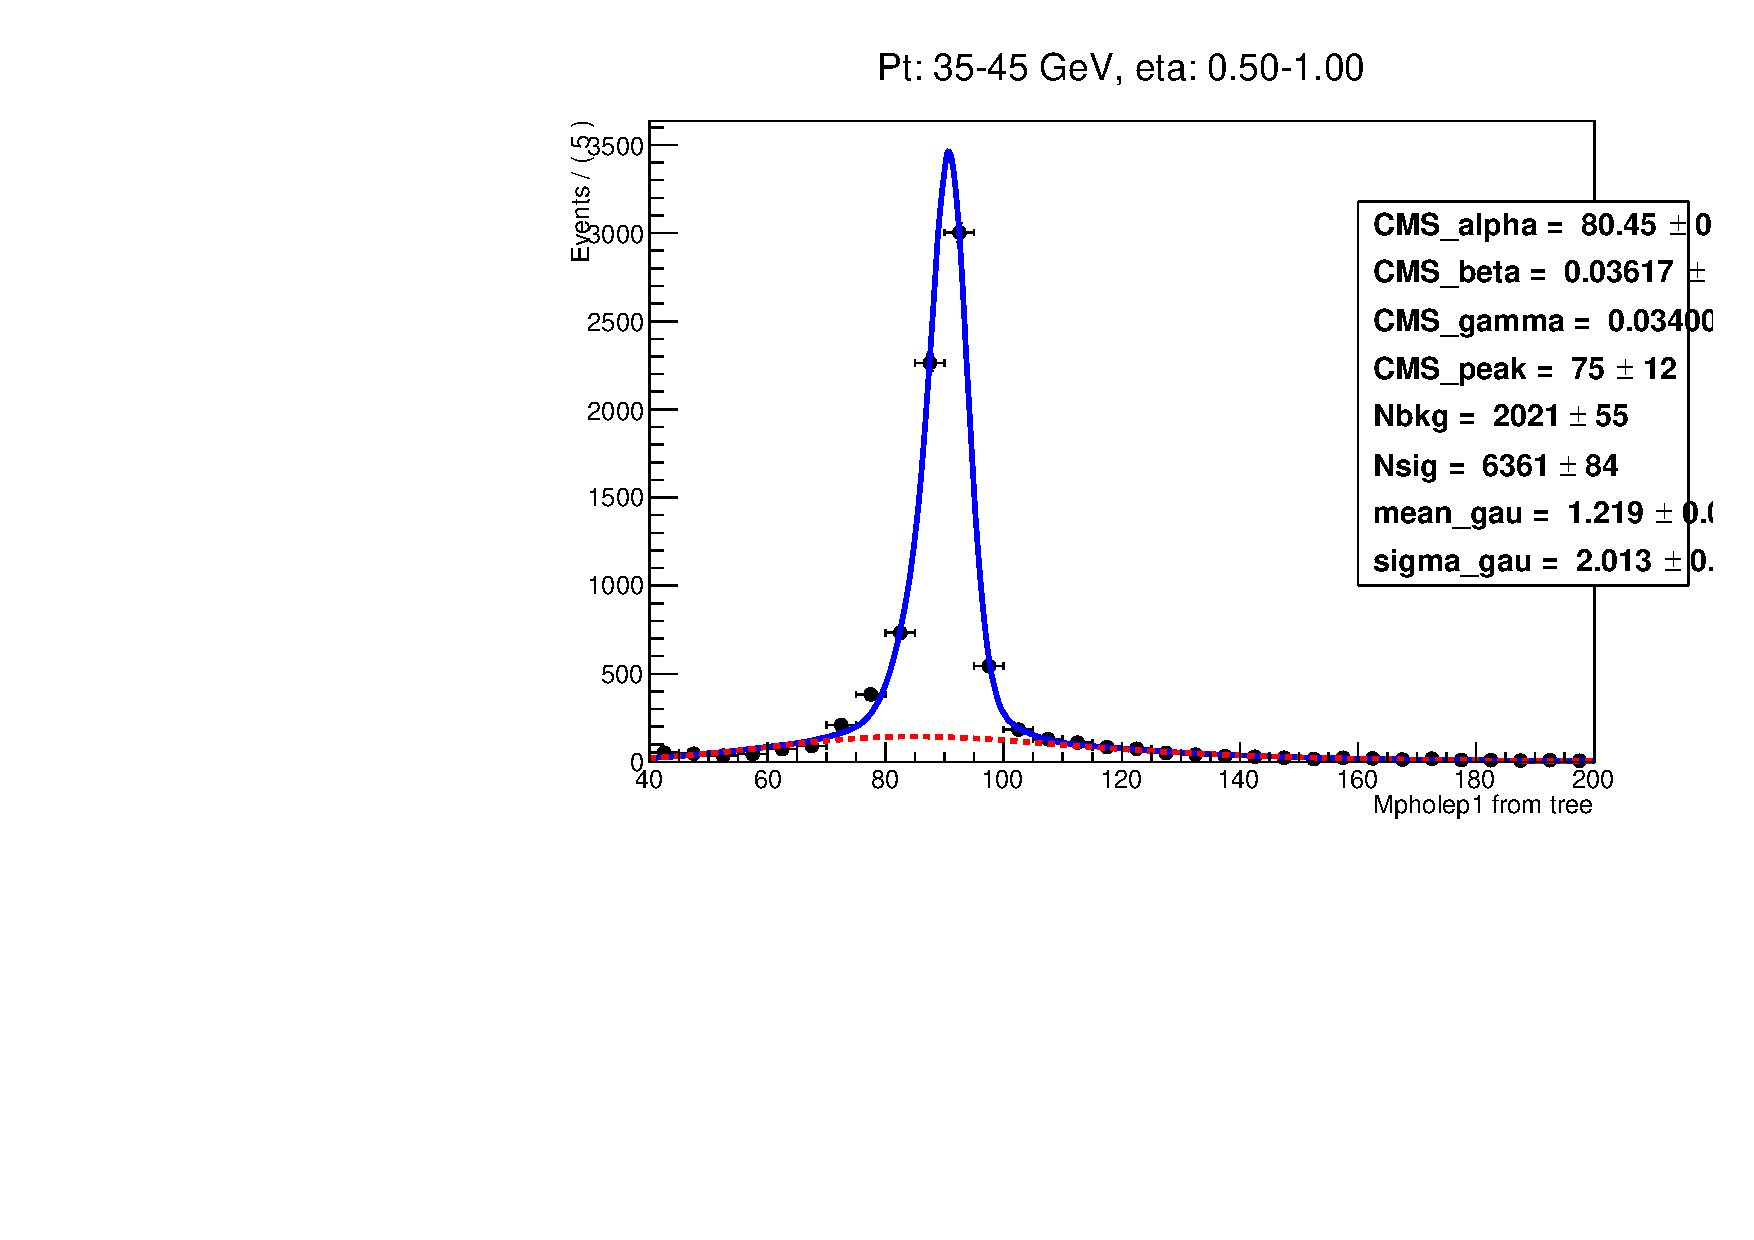
\includegraphics[width=0.45\textwidth]{../figs/figs_v11/ELECTRON_WGamma/EtoGammaFits/sa_hZmass_h_Data_EtoGamma_Enr_BARREL_pt35to45_ieta2.pdf}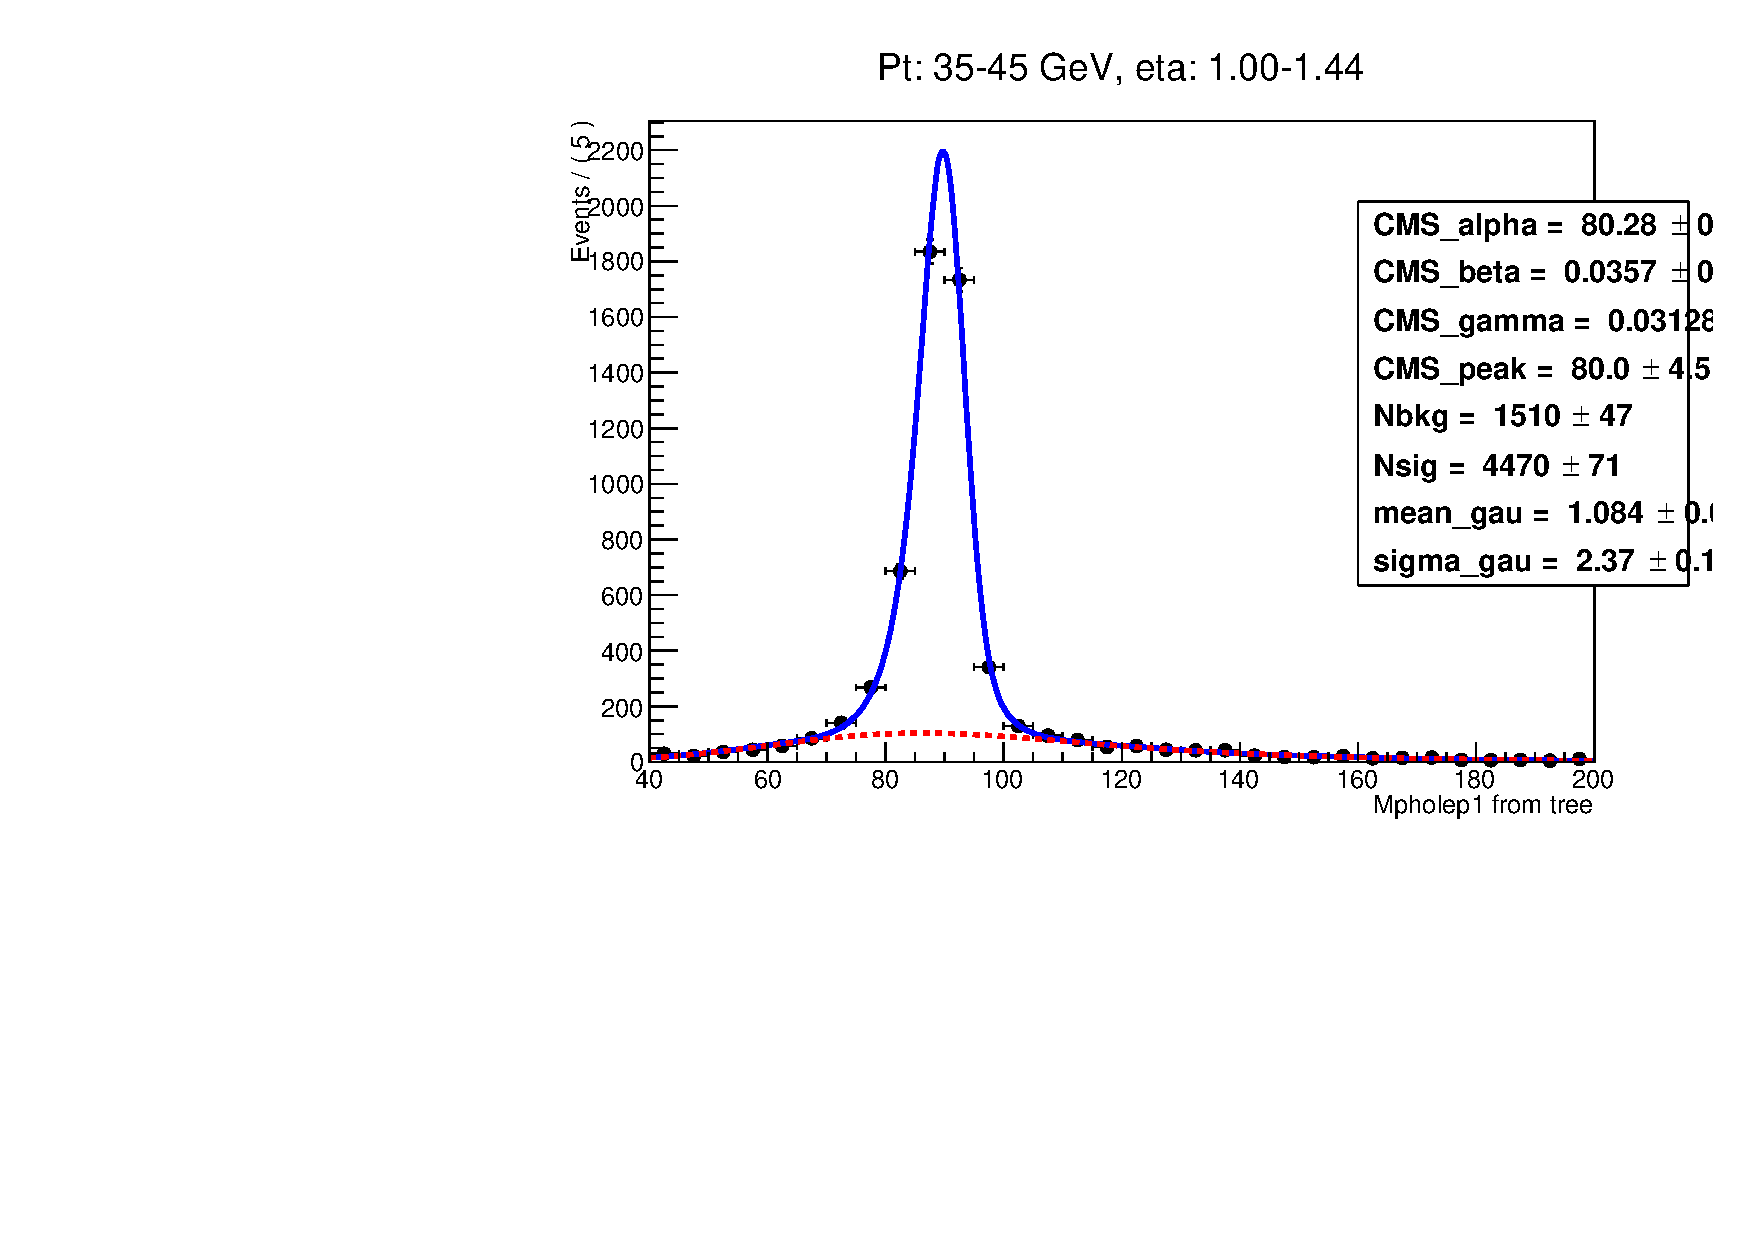
\includegraphics[width=0.45\textwidth]{../figs/figs_v11/ELECTRON_WGamma/EtoGammaFits/sa_hZmass_h_Data_EtoGamma_Enr_BARREL_pt35to45_ieta3.pdf}\\
   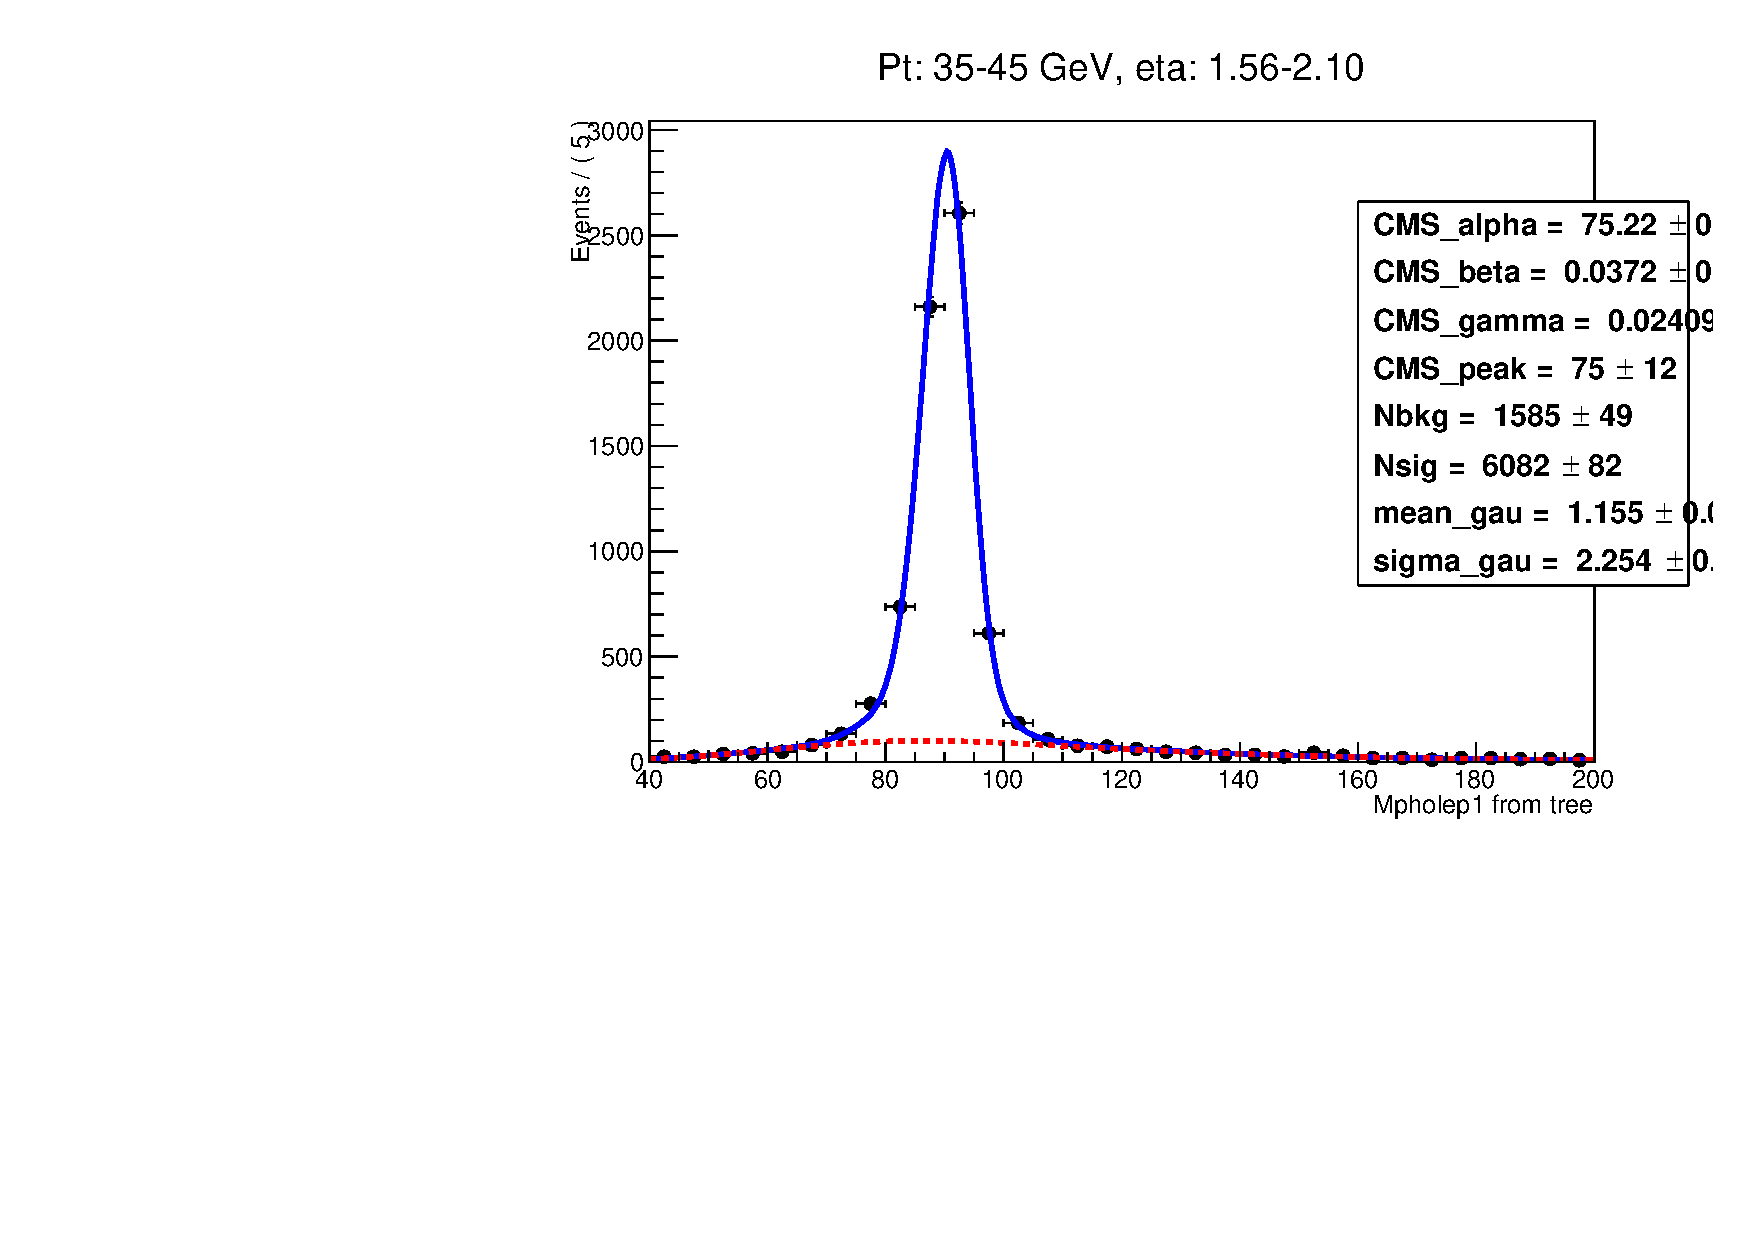
\includegraphics[width=0.45\textwidth]{../figs/figs_v11/ELECTRON_WGamma/EtoGammaFits/sa_hZmass_h_Data_EtoGamma_Enr_ENDCAP_pt35to45_ieta0.pdf}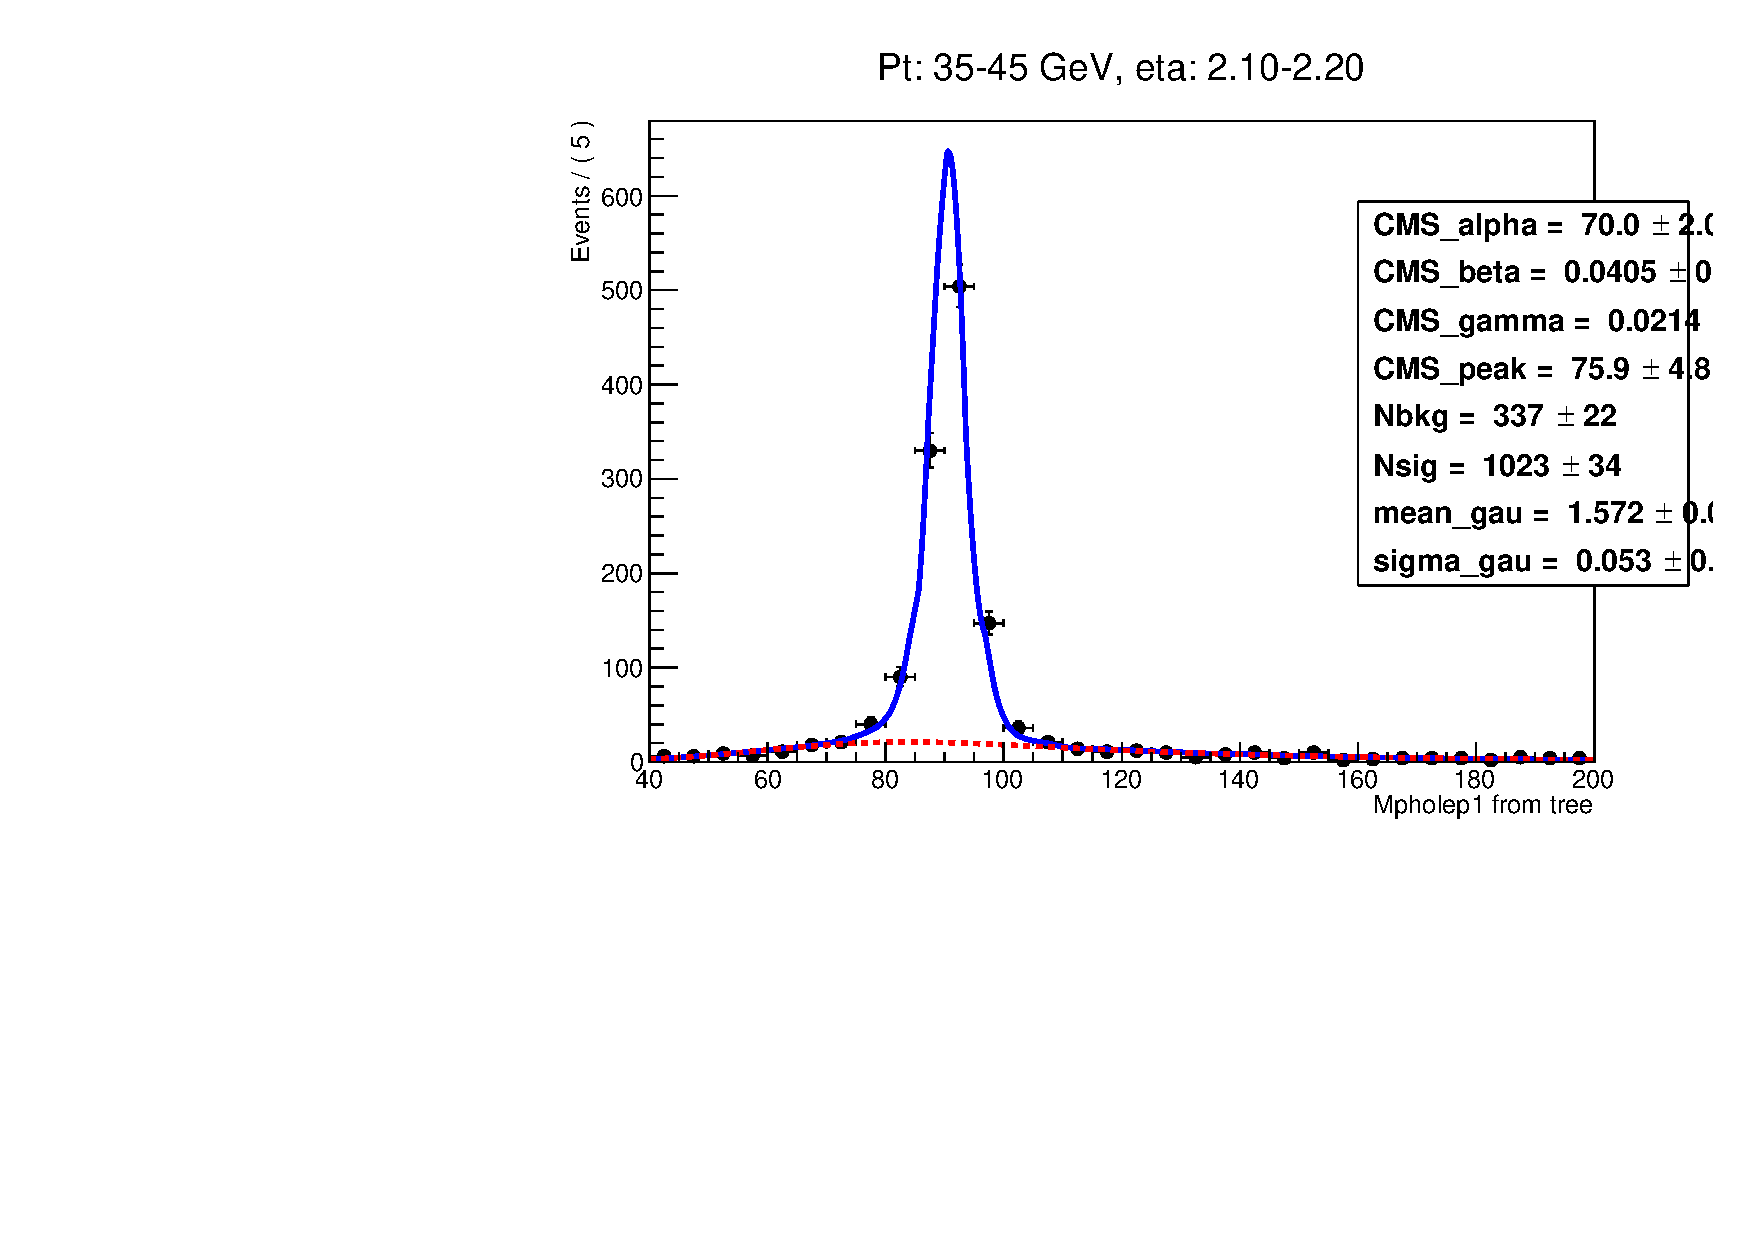
\includegraphics[width=0.45\textwidth]{../figs/figs_v11/ELECTRON_WGamma/EtoGammaFits/sa_hZmass_h_Data_EtoGamma_Enr_ENDCAP_pt35to45_ieta1.pdf}\\
   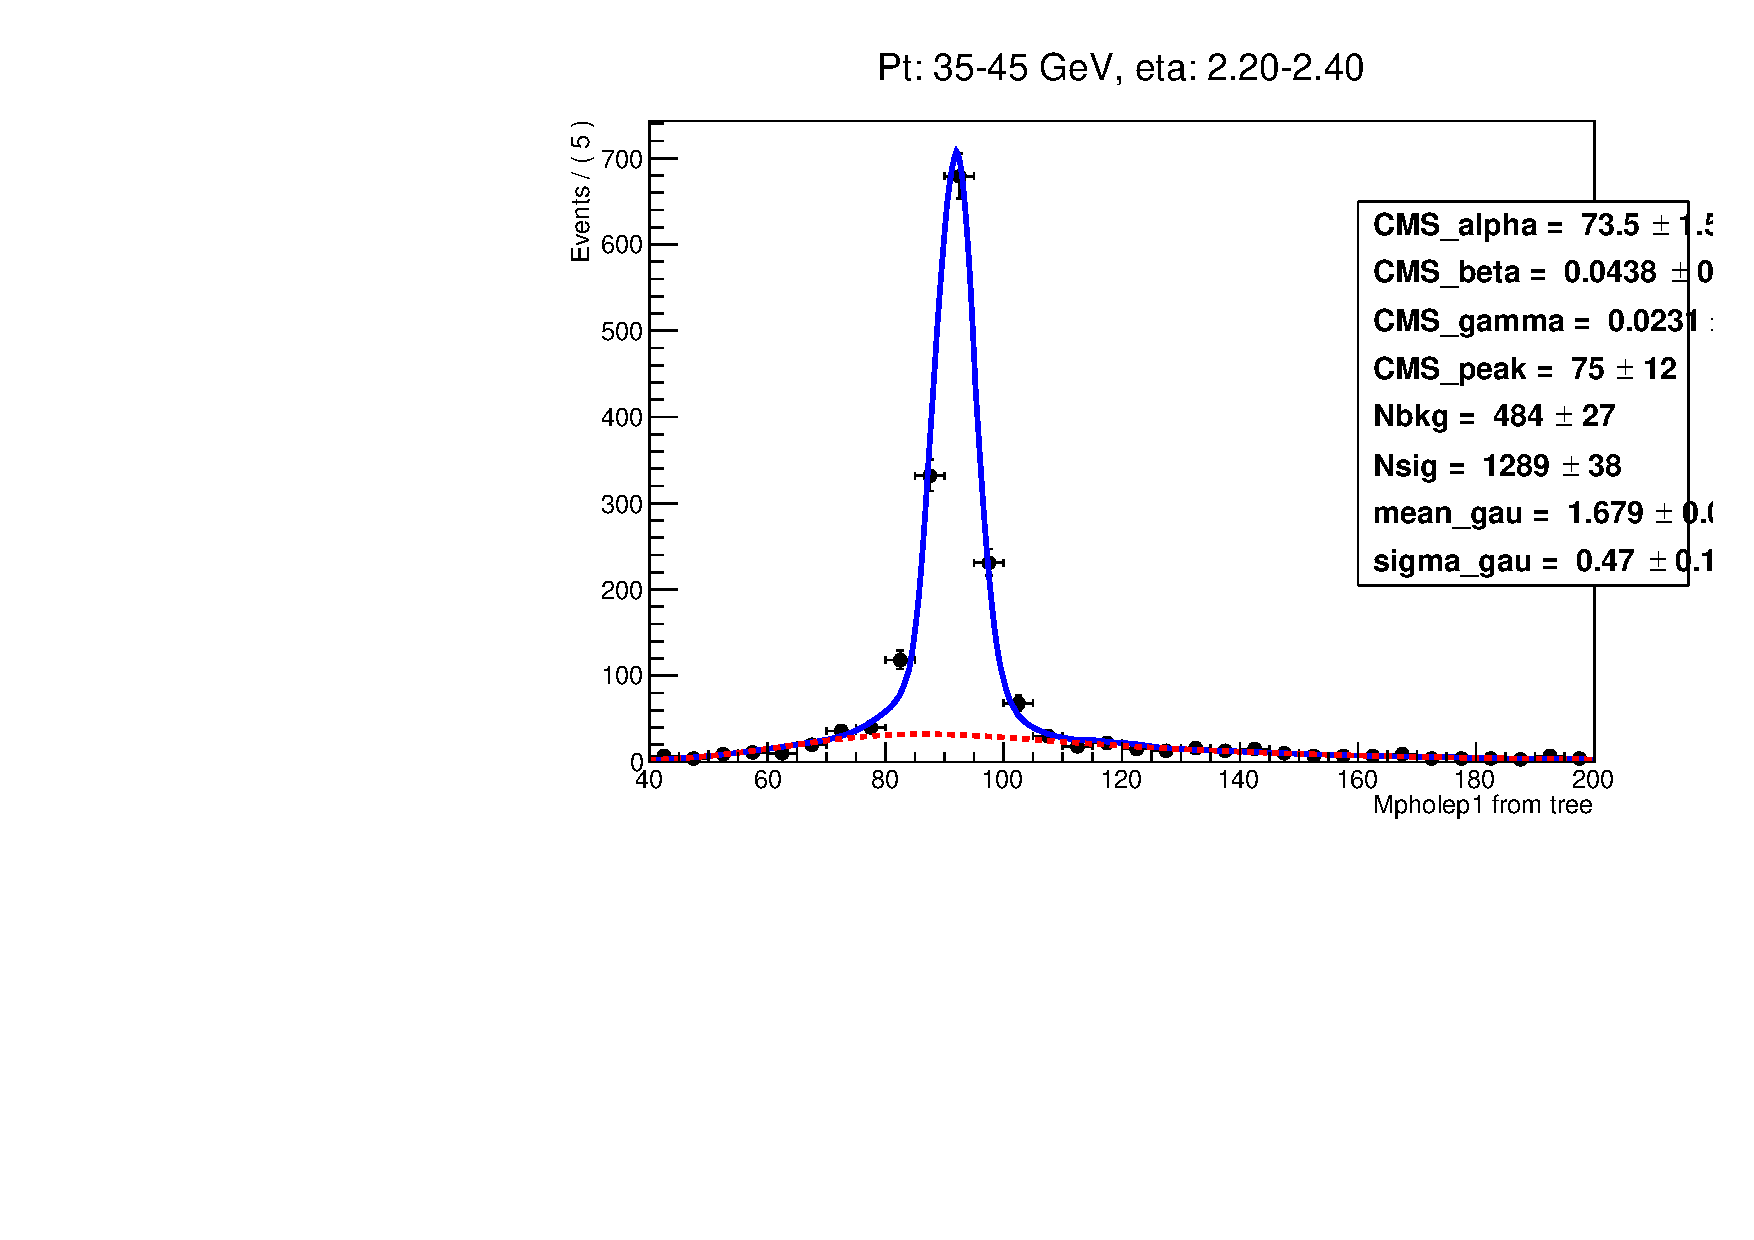
\includegraphics[width=0.45\textwidth]{../figs/figs_v11/ELECTRON_WGamma/EtoGammaFits/sa_hZmass_h_Data_EtoGamma_Enr_ENDCAP_pt35to45_ieta2.pdf}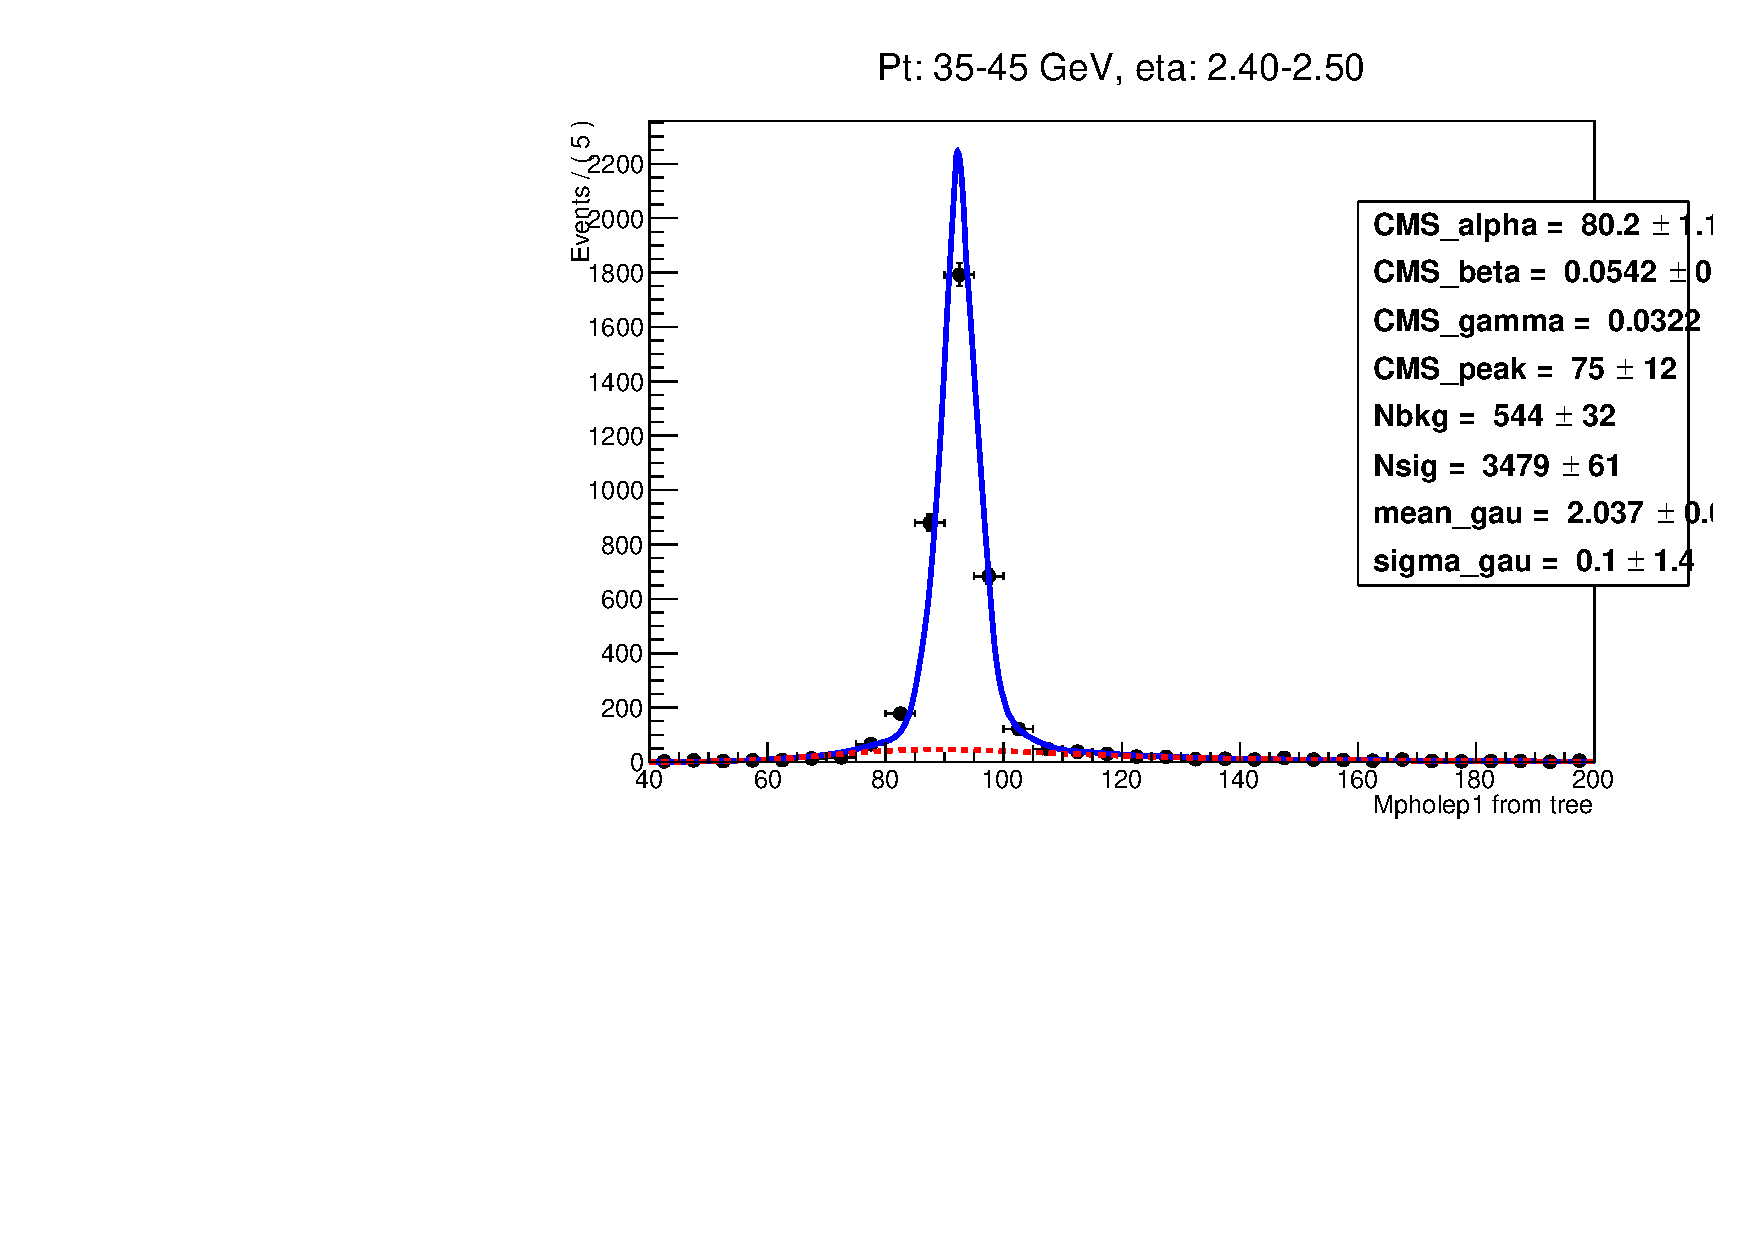
\includegraphics[width=0.45\textwidth]{../figs/figs_v11/ELECTRON_WGamma/EtoGammaFits/sa_hZmass_h_Data_EtoGamma_Enr_ENDCAP_pt35to45_ieta3.pdf}\\
  \label{fig:etogFits_35to45}
  \caption{$M_{e,\gamma}$ fits, W$\gamma$, electron channel, underflow bin (35-45 GeV), 8 eta bins}
  \end{center}
\end{figure}

\begin{figure}[htb]
  \begin{center}
   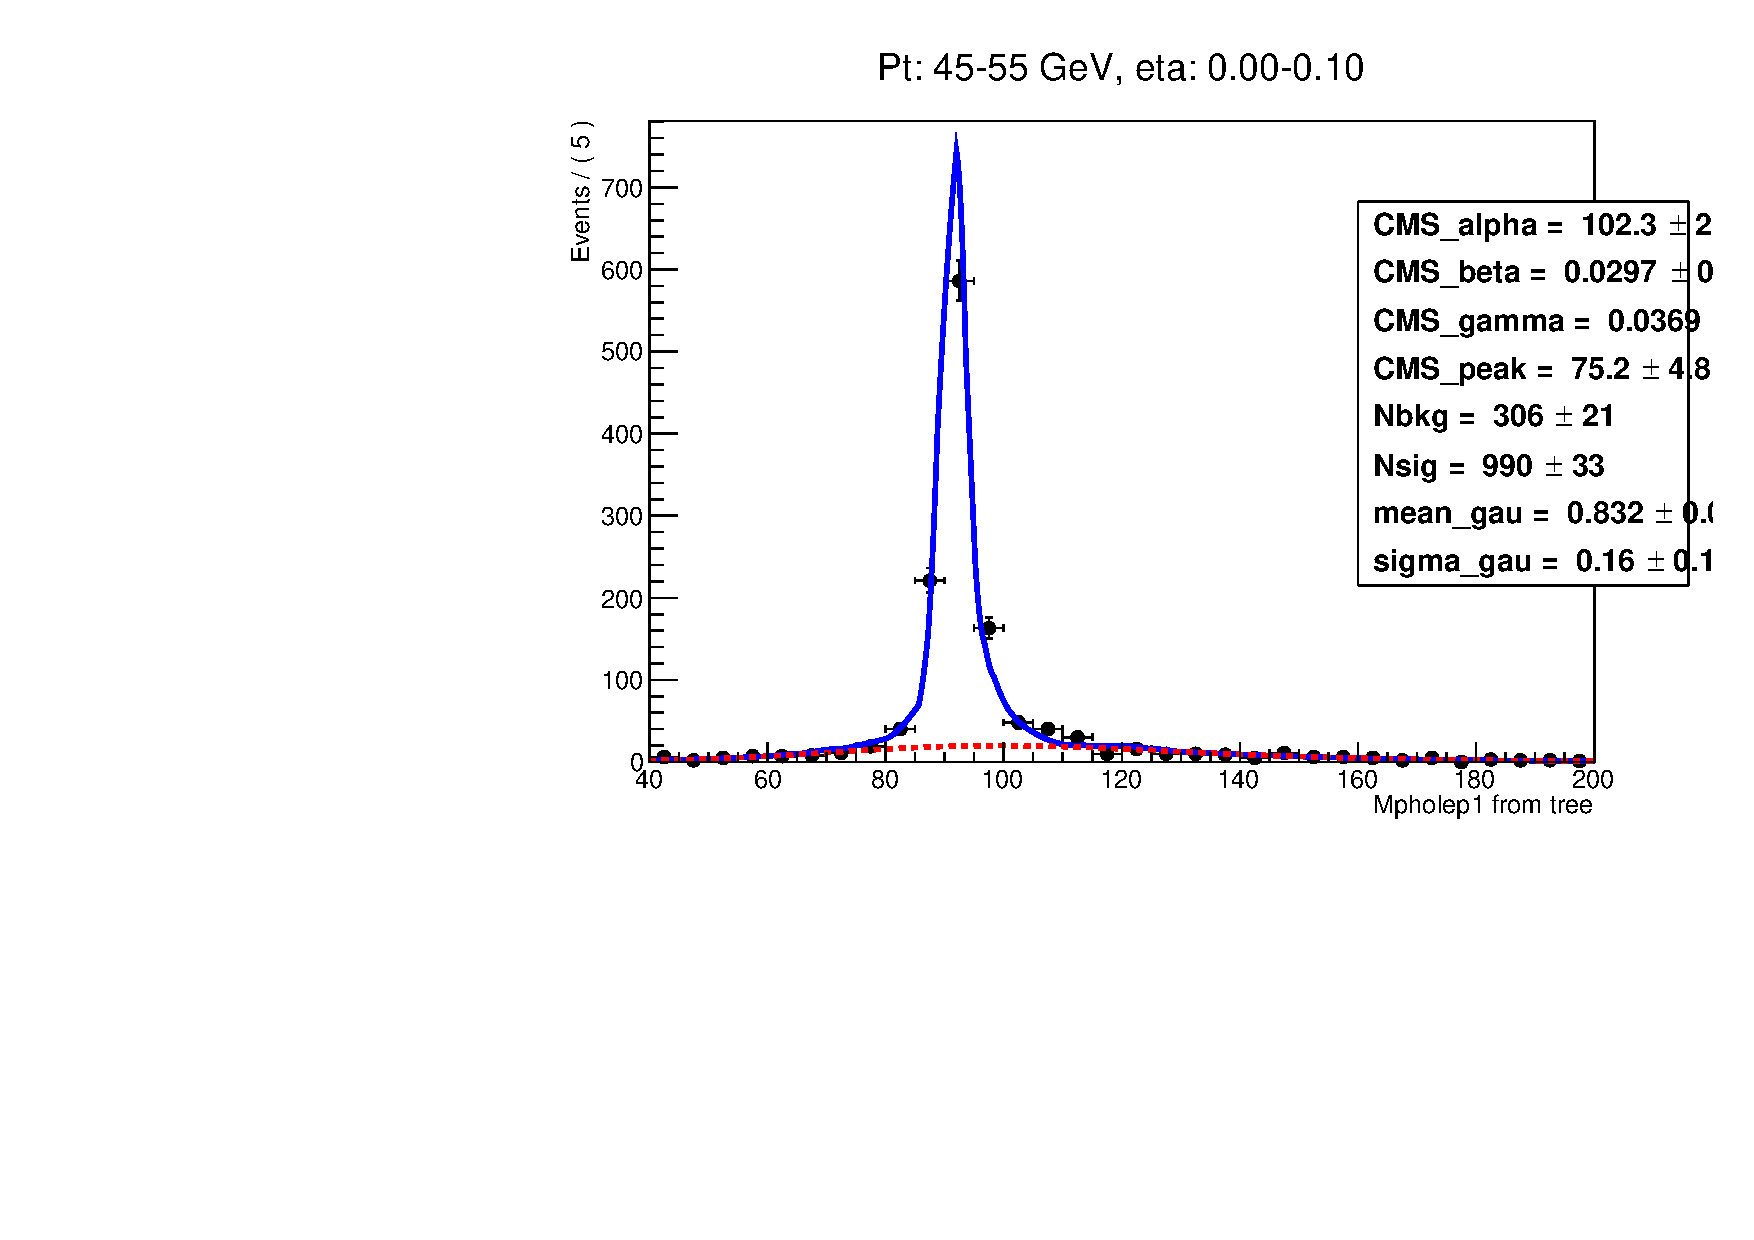
\includegraphics[width=0.45\textwidth]{../figs/figs_v11/ELECTRON_WGamma/EtoGammaFits/sa_hZmass_h_Data_EtoGamma_Enr_BARREL_pt45to55_ieta0.pdf}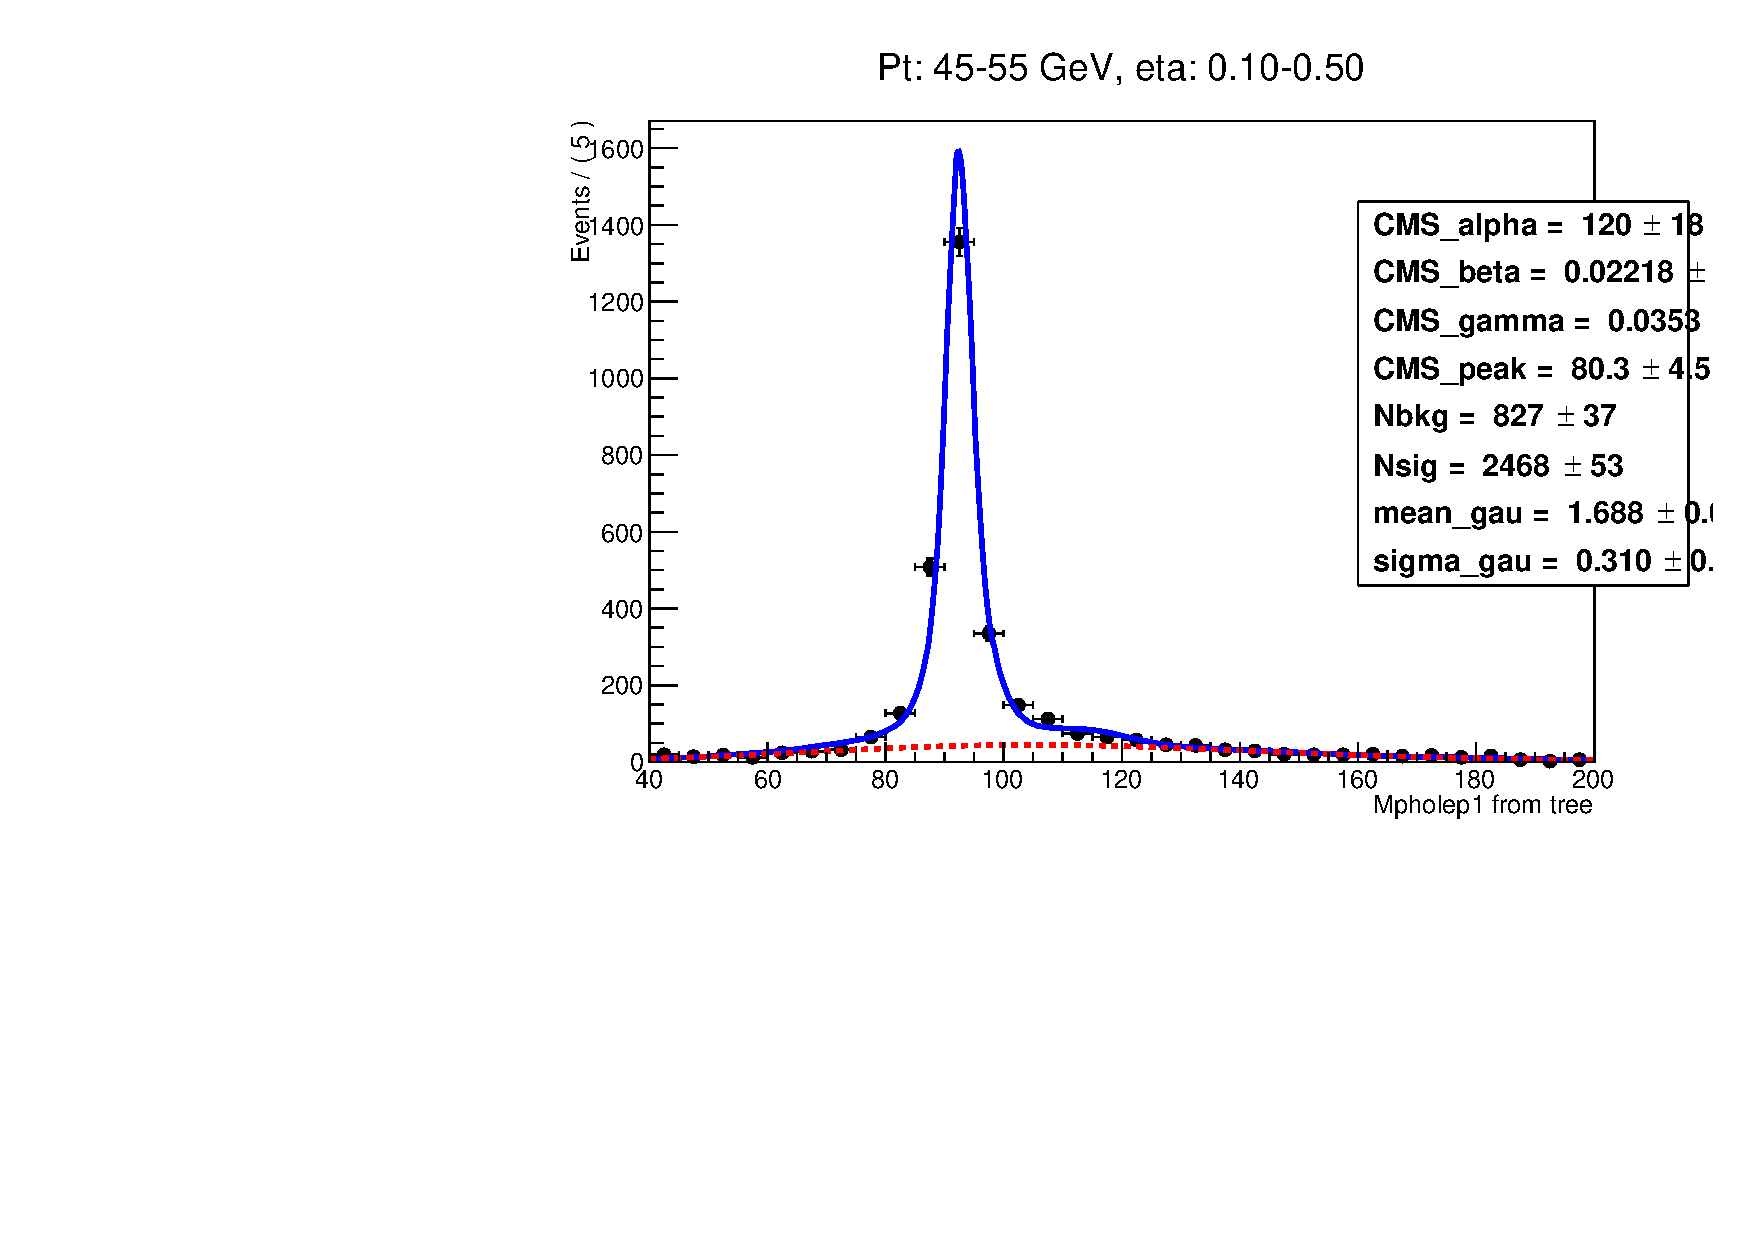
\includegraphics[width=0.45\textwidth]{../figs/figs_v11/ELECTRON_WGamma/EtoGammaFits/sa_hZmass_h_Data_EtoGamma_Enr_BARREL_pt45to55_ieta1.pdf}\\
   \includegraphics[width=0.45\textwidth]{../figs/figs_v11/ELECTRON_WGamma/EtoGammaFits/sa_hZmass_h_Data_EtoGamma_Enr_BARREL_pt45to55_ieta2.pdf}\includegraphics[width=0.45\textwidth]{../figs/figs_v11/ELECTRON_WGamma/EtoGammaFits/sa_hZmass_h_Data_EtoGamma_Enr_BARREL_pt45to55_ieta3.pdf}\\
   \includegraphics[width=0.45\textwidth]{../figs/figs_v11/ELECTRON_WGamma/EtoGammaFits/sa_hZmass_h_Data_EtoGamma_Enr_ENDCAP_pt45to55_ieta0.pdf}\includegraphics[width=0.45\textwidth]{../figs/figs_v11/ELECTRON_WGamma/EtoGammaFits/sa_hZmass_h_Data_EtoGamma_Enr_ENDCAP_pt45to55_ieta1.pdf}\\
   \includegraphics[width=0.45\textwidth]{../figs/figs_v11/ELECTRON_WGamma/EtoGammaFits/sa_hZmass_h_Data_EtoGamma_Enr_ENDCAP_pt45to55_ieta2.pdf}\includegraphics[width=0.45\textwidth]{../figs/figs_v11/ELECTRON_WGamma/EtoGammaFits/sa_hZmass_h_Data_EtoGamma_Enr_ENDCAP_pt45to55_ieta3.pdf}\\
  \label{fig:etogFits_45to55}
  \caption{$M_{e,\gamma}$ fits, W$\gamma$, electron channel, underflow bin (45-55 GeV), 8 eta bins}
  \end{center}
\end{figure}

\begin{figure}[htb]
  \begin{center}
   \includegraphics[width=0.45\textwidth]{../figs/figs_v11/ELECTRON_WGamma/EtoGammaFits/sa_hZmass_h_Data_EtoGamma_Enr_BARREL_pt55to65_ieta0.pdf}\includegraphics[width=0.45\textwidth]{../figs/figs_v11/ELECTRON_WGamma/EtoGammaFits/sa_hZmass_h_Data_EtoGamma_Enr_BARREL_pt55to65_ieta1.pdf}\\
   \includegraphics[width=0.45\textwidth]{../figs/figs_v11/ELECTRON_WGamma/EtoGammaFits/sa_hZmass_h_Data_EtoGamma_Enr_ENDCAP_pt55to65_ieta0.pdf}\includegraphics[width=0.45\textwidth]{../figs/figs_v11/ELECTRON_WGamma/EtoGammaFits/sa_hZmass_h_Data_EtoGamma_Enr_ENDCAP_pt55to65_ieta1.pdf}\\
  \label{fig:etogFits_55to65}
  \caption{$M_{e,\gamma}$ fits, W$\gamma$, electron channel, underflow bin (55-65 GeV), 4 eta bins}
  \end{center}
\end{figure}

\begin{figure}[htb]
  \begin{center}
   \includegraphics[width=0.45\textwidth]{../figs/figs_v11/ELECTRON_WGamma/EtoGammaFits/sa_hZmass_h_Data_EtoGamma_Enr_BARREL_pt65to75_ieta0.pdf}\includegraphics[width=0.45\textwidth]{../figs/figs_v11/ELECTRON_WGamma/EtoGammaFits/sa_hZmass_h_Data_EtoGamma_Enr_BARREL_pt65to75_ieta1.pdf}\\
   \includegraphics[width=0.45\textwidth]{../figs/figs_v11/ELECTRON_WGamma/EtoGammaFits/sa_hZmass_h_Data_EtoGamma_Enr_ENDCAP_pt65to75_ieta0.pdf}\includegraphics[width=0.45\textwidth]{../figs/figs_v11/ELECTRON_WGamma/EtoGammaFits/sa_hZmass_h_Data_EtoGamma_Enr_ENDCAP_pt65to75_ieta1.pdf}\\
  \label{fig:etogFits_65to75}
  \caption{$M_{e,\gamma}$ fits, W$\gamma$, electron channel, underflow bin (65-75 GeV), 4 eta bins}
  \end{center}
\end{figure}


\begin{figure}[htb]
  \begin{center}
   \includegraphics[width=0.45\textwidth]{../figs/figs_v11/ELECTRON_WGamma/EtoGammaFits/sa_hZmass_h_Data_EtoGamma_Enr_BARREL_pt75to85_ieta0.pdf}\includegraphics[width=0.45\textwidth]{../figs/figs_v11/ELECTRON_WGamma/EtoGammaFits/sa_hZmass_h_Data_EtoGamma_Enr_BARREL_pt75to85_ieta1.pdf}\\
   \includegraphics[width=0.45\textwidth]{../figs/figs_v11/ELECTRON_WGamma/EtoGammaFits/sa_hZmass_h_Data_EtoGamma_Enr_ENDCAP_pt75to85_ieta0.pdf}\includegraphics[width=0.45\textwidth]{../figs/figs_v11/ELECTRON_WGamma/EtoGammaFits/sa_hZmass_h_Data_EtoGamma_Enr_ENDCAP_pt75to85_ieta1.pdf}\\
  \label{fig:etogFits_75to85}
  \caption{$M_{e,\gamma}$ fits, W$\gamma$, electron channel, underflow bin (75-85 GeV), 4 eta bins}
  \end{center}
\end{figure}

\begin{figure}[htb]
  \begin{center}
   \includegraphics[width=0.45\textwidth]{../figs/figs_v11/ELECTRON_WGamma/EtoGammaFits/sa_hZmass_h_Data_EtoGamma_Enr_BARREL_pt85to95_ieta0.pdf}
   \includegraphics[width=0.45\textwidth]{../figs/figs_v11/ELECTRON_WGamma/EtoGammaFits/sa_hZmass_h_Data_EtoGamma_Enr_ENDCAP_pt85to95_ieta0.pdf}\\
  \label{fig:etogFits_85to95}
  \caption{$M_{e,\gamma}$ fits, W$\gamma$, electron channel, underflow bin (85-95 GeV), 2 eta bins}
  \end{center}
\end{figure}

\begin{figure}[htb]
  \begin{center}
   \includegraphics[width=0.45\textwidth]{../figs/figs_v11/ELECTRON_WGamma/EtoGammaFits/sa_hZmass_h_Data_EtoGamma_Enr_BARREL_pt95to120_ieta0.pdf}
   \includegraphics[width=0.45\textwidth]{../figs/figs_v11/ELECTRON_WGamma/EtoGammaFits/sa_hZmass_h_Data_EtoGamma_Enr_ENDCAP_pt95to120_ieta0.pdf}\\
  \label{fig:etogFits_95to120}
  \caption{$M_{e,\gamma}$ fits, W$\gamma$, electron channel, underflow bin (95-120 GeV), 2 eta bins}
  \end{center}
\end{figure}

\begin{figure}[htb]
  \begin{center}
   \includegraphics[width=0.45\textwidth]{../figs/figs_v11/ELECTRON_WGamma/EtoGammaFits/sa_hZmass_h_Data_EtoGamma_Enr_BARREL_pt120to500_ieta0.pdf}
   \includegraphics[width=0.45\textwidth]{../figs/figs_v11/ELECTRON_WGamma/EtoGammaFits/sa_hZmass_h_Data_EtoGamma_Enr_ENDCAP_pt120to500_ieta0.pdf}\\
  \label{fig:etogFits_120to500}
  \caption{$M_{e,\gamma}$ fits, W$\gamma$, electron channel, underflow bin (120-500 GeV), 2 eta bins}
  \end{center}
\end{figure}


